\documentclass[twoside]{book}

% Packages required by doxygen
\usepackage{calc}
\usepackage{doxygen}
\usepackage{graphicx}
\usepackage[utf8]{inputenc}
\usepackage{makeidx}
\usepackage{multicol}
\usepackage{multirow}
\usepackage{textcomp}
\usepackage[table]{xcolor}

% Font selection
\usepackage[T1]{fontenc}
\usepackage{mathptmx}
\usepackage[scaled=.90]{helvet}
\usepackage{courier}
\usepackage{amssymb}
\usepackage{sectsty}
\renewcommand{\familydefault}{\sfdefault}
\allsectionsfont{%
  \fontseries{bc}\selectfont%
  \color{darkgray}%
}
\renewcommand{\DoxyLabelFont}{%
  \fontseries{bc}\selectfont%
  \color{darkgray}%
}

% Page & text layout
\usepackage{geometry}
\geometry{%
  a4paper,%
  top=2.5cm,%
  bottom=2.5cm,%
  left=2.5cm,%
  right=2.5cm%
}
\tolerance=750
\hfuzz=15pt
\hbadness=750
\setlength{\emergencystretch}{15pt}
\setlength{\parindent}{0cm}
\setlength{\parskip}{0.2cm}
\makeatletter
\renewcommand{\paragraph}{%
  \@startsection{paragraph}{4}{0ex}{-1.0ex}{1.0ex}{%
    \normalfont\normalsize\bfseries\SS@parafont%
  }%
}
\renewcommand{\subparagraph}{%
  \@startsection{subparagraph}{5}{0ex}{-1.0ex}{1.0ex}{%
    \normalfont\normalsize\bfseries\SS@subparafont%
  }%
}
\makeatother

% Headers & footers
\usepackage{fancyhdr}
\pagestyle{fancyplain}
\fancyhead[LE]{\fancyplain{}{\bfseries\thepage}}
\fancyhead[CE]{\fancyplain{}{}}
\fancyhead[RE]{\fancyplain{}{\bfseries\leftmark}}
\fancyhead[LO]{\fancyplain{}{\bfseries\rightmark}}
\fancyhead[CO]{\fancyplain{}{}}
\fancyhead[RO]{\fancyplain{}{\bfseries\thepage}}
\fancyfoot[LE]{\fancyplain{}{}}
\fancyfoot[CE]{\fancyplain{}{}}
\fancyfoot[RE]{\fancyplain{}{\bfseries\scriptsize Generated on Fri Nov 30 2018 19\-:52\-:16 for pymtt by Doxygen }}
\fancyfoot[LO]{\fancyplain{}{\bfseries\scriptsize Generated on Fri Nov 30 2018 19\-:52\-:16 for pymtt by Doxygen }}
\fancyfoot[CO]{\fancyplain{}{}}
\fancyfoot[RO]{\fancyplain{}{}}
\renewcommand{\footrulewidth}{0.4pt}
\renewcommand{\chaptermark}[1]{%
  \markboth{#1}{}%
}
\renewcommand{\sectionmark}[1]{%
  \markright{\thesection\ #1}%
}

% Indices & bibliography
\usepackage{natbib}
\usepackage[titles]{tocloft}
\setcounter{tocdepth}{3}
\setcounter{secnumdepth}{5}
\makeindex

% Hyperlinks (required, but should be loaded last)
\usepackage{ifpdf}
\ifpdf
  \usepackage[pdftex,pagebackref=true]{hyperref}
\else
  \usepackage[ps2pdf,pagebackref=true]{hyperref}
\fi
\hypersetup{%
  colorlinks=true,%
  linkcolor=blue,%
  citecolor=blue,%
  unicode%
}

% Custom commands
\newcommand{\clearemptydoublepage}{%
  \newpage{\pagestyle{empty}\cleardoublepage}%
}


%===== C O N T E N T S =====

\begin{document}

% Titlepage & ToC
\hypersetup{pageanchor=false}
\pagenumbering{roman}
\begin{titlepage}
\vspace*{7cm}
\begin{center}%
{\Large pymtt }\\
\vspace*{1cm}
{\large Generated by Doxygen 1.8.6}\\
\vspace*{0.5cm}
{\small Fri Nov 30 2018 19:52:16}\\
\end{center}
\end{titlepage}
\clearemptydoublepage
\tableofcontents
\clearemptydoublepage
\pagenumbering{arabic}
\hypersetup{pageanchor=true}

%--- Begin generated contents ---
\chapter{Namespace Index}
\section{Packages}
Here are the packages with brief descriptions (if available)\-:\begin{DoxyCompactList}
\item\contentsline{section}{\hyperlink{namespaceALPS}{A\-L\-P\-S} }{\pageref{namespaceALPS}}{}
\item\contentsline{section}{\hyperlink{namespaceAlreadyInstalled}{Already\-Installed} }{\pageref{namespaceAlreadyInstalled}}{}
\item\contentsline{section}{\hyperlink{namespaceAutotools}{Autotools} }{\pageref{namespaceAutotools}}{}
\item\contentsline{section}{\hyperlink{namespaceBaseMTTUtility}{Base\-M\-T\-T\-Utility} }{\pageref{namespaceBaseMTTUtility}}{}
\item\contentsline{section}{\hyperlink{namespaceBIOSMTTStage}{B\-I\-O\-S\-M\-T\-T\-Stage} }{\pageref{namespaceBIOSMTTStage}}{}
\item\contentsline{section}{\hyperlink{namespaceBuildMTTTool}{Build\-M\-T\-T\-Tool} }{\pageref{namespaceBuildMTTTool}}{}
\item\contentsline{section}{\hyperlink{namespaceCNCMTTTool}{C\-N\-C\-M\-T\-T\-Tool} }{\pageref{namespaceCNCMTTTool}}{}
\item\contentsline{section}{\hyperlink{namespacecombinatorial}{combinatorial} }{\pageref{namespacecombinatorial}}{}
\item\contentsline{section}{\hyperlink{namespaceCompilers}{Compilers} }{\pageref{namespaceCompilers}}{}
\item\contentsline{section}{\hyperlink{namespaceCopytree}{Copytree} }{\pageref{namespaceCopytree}}{}
\item\contentsline{section}{\hyperlink{namespaceDefaultMTTDefaults}{Default\-M\-T\-T\-Defaults} }{\pageref{namespaceDefaultMTTDefaults}}{}
\item\contentsline{section}{\hyperlink{namespaceDefaultProfile}{Default\-Profile} }{\pageref{namespaceDefaultProfile}}{}
\item\contentsline{section}{\hyperlink{namespaceDefaultTestBuild}{Default\-Test\-Build} }{\pageref{namespaceDefaultTestBuild}}{}
\item\contentsline{section}{\hyperlink{namespacedeveloper}{developer} }{\pageref{namespacedeveloper}}{}
\item\contentsline{section}{\hyperlink{namespaceEnviron}{Environ} }{\pageref{namespaceEnviron}}{}
\item\contentsline{section}{\hyperlink{namespaceExecuteCmd}{Execute\-Cmd} }{\pageref{namespaceExecuteCmd}}{}
\item\contentsline{section}{\hyperlink{namespaceExecutorMTTTool}{Executor\-M\-T\-T\-Tool} }{\pageref{namespaceExecutorMTTTool}}{}
\item\contentsline{section}{\hyperlink{namespaceFetchMTTTool}{Fetch\-M\-T\-T\-Tool} }{\pageref{namespaceFetchMTTTool}}{}
\item\contentsline{section}{\hyperlink{namespaceFirmwareMTTStage}{Firmware\-M\-T\-T\-Stage} }{\pageref{namespaceFirmwareMTTStage}}{}
\item\contentsline{section}{\hyperlink{namespaceFooFlash}{Foo\-Flash} }{\pageref{namespaceFooFlash}}{}
\item\contentsline{section}{\hyperlink{namespaceftb}{ftb} }{\pageref{namespaceftb}}{}
\item\contentsline{section}{\hyperlink{namespacefull-trivial}{full-\/trivial} }{\pageref{namespacefull-trivial}}{}
\item\contentsline{section}{\hyperlink{namespacegds-demo}{gds-\/demo} }{\pageref{namespacegds-demo}}{}
\item\contentsline{section}{\hyperlink{namespaceGit}{Git} }{\pageref{namespaceGit}}{}
\item\contentsline{section}{\hyperlink{namespaceharasser}{harasser} }{\pageref{namespaceharasser}}{}
\item\contentsline{section}{\hyperlink{namespaceHarasser}{Harasser} }{\pageref{namespaceHarasser}}{}
\item\contentsline{section}{\hyperlink{namespaceHarasserMTTTool}{Harasser\-M\-T\-T\-Tool} }{\pageref{namespaceHarasserMTTTool}}{}
\item\contentsline{section}{\hyperlink{namespaceHostfile}{Hostfile} }{\pageref{namespaceHostfile}}{}
\item\contentsline{section}{\hyperlink{namespacehwtest}{hwtest} }{\pageref{namespacehwtest}}{}
\item\contentsline{section}{\hyperlink{namespaceintel}{intel} }{\pageref{namespaceintel}}{}
\item\contentsline{section}{\hyperlink{namespaceIPMITool}{I\-P\-M\-I\-Tool} }{\pageref{namespaceIPMITool}}{}
\item\contentsline{section}{\hyperlink{namespaceIUDatabase}{I\-U\-Database} }{\pageref{namespaceIUDatabase}}{}
\item\contentsline{section}{\hyperlink{namespaceJunitXML}{Junit\-X\-M\-L} }{\pageref{namespaceJunitXML}}{}
\item\contentsline{section}{\hyperlink{namespaceLauncherDefaultsMTTStage}{Launcher\-Defaults\-M\-T\-T\-Stage} }{\pageref{namespaceLauncherDefaultsMTTStage}}{}
\item\contentsline{section}{\hyperlink{namespaceLauncherMTTTool}{Launcher\-M\-T\-T\-Tool} }{\pageref{namespaceLauncherMTTTool}}{}
\item\contentsline{section}{\hyperlink{namespaceLoadClasses}{Load\-Classes} }{\pageref{namespaceLoadClasses}}{}
\item\contentsline{section}{\hyperlink{namespaceLogger}{Logger} }{\pageref{namespaceLogger}}{}
\item\contentsline{section}{\hyperlink{namespaceMiddlewareBuildMTTStage}{Middleware\-Build\-M\-T\-T\-Stage} }{\pageref{namespaceMiddlewareBuildMTTStage}}{}
\item\contentsline{section}{\hyperlink{namespaceMiddlewareGetMTTStage}{Middleware\-Get\-M\-T\-T\-Stage} }{\pageref{namespaceMiddlewareGetMTTStage}}{}
\item\contentsline{section}{\hyperlink{namespaceModuleCmd}{Module\-Cmd} }{\pageref{namespaceModuleCmd}}{}
\item\contentsline{section}{\hyperlink{namespacempich2-template}{mpich2-\/template} }{\pageref{namespacempich2-template}}{}
\item\contentsline{section}{\hyperlink{namespacempitest}{mpitest} }{\pageref{namespacempitest}}{}
\item\contentsline{section}{\hyperlink{namespaceMPIVersion}{M\-P\-I\-Version} }{\pageref{namespaceMPIVersion}}{}
\item\contentsline{section}{\hyperlink{namespaceMTTDefaultsMTTStage}{M\-T\-T\-Defaults\-M\-T\-T\-Stage} }{\pageref{namespaceMTTDefaultsMTTStage}}{}
\item\contentsline{section}{\hyperlink{namespaceMTTVersionPlugin}{M\-T\-T\-Version\-Plugin} }{\pageref{namespaceMTTVersionPlugin}}{}
\item\contentsline{section}{\hyperlink{namespaceompi-core-perf-testing}{ompi-\/core-\/perf-\/testing} }{\pageref{namespaceompi-core-perf-testing}}{}
\item\contentsline{section}{\hyperlink{namespaceompi-core-template}{ompi-\/core-\/template} }{\pageref{namespaceompi-core-template}}{}
\item\contentsline{section}{\hyperlink{namespaceompi__hello__world}{ompi\-\_\-hello\-\_\-world} }{\pageref{namespaceompi__hello__world}}{}
\item\contentsline{section}{\hyperlink{namespaceOMPI__Snapshot}{O\-M\-P\-I\-\_\-\-Snapshot} }{\pageref{namespaceOMPI__Snapshot}}{}
\item\contentsline{section}{\hyperlink{namespaceompi__snapshot__seq}{ompi\-\_\-snapshot\-\_\-seq} }{\pageref{namespaceompi__snapshot__seq}}{}
\item\contentsline{section}{\hyperlink{namespaceOpenMPI}{Open\-M\-P\-I} }{\pageref{namespaceOpenMPI}}{}
\item\contentsline{section}{\hyperlink{namespaceopenshmem__tests__patch}{openshmem\-\_\-tests\-\_\-patch} }{\pageref{namespaceopenshmem__tests__patch}}{}
\item\contentsline{section}{\hyperlink{namespaceoshmem}{oshmem} }{\pageref{namespaceoshmem}}{}
\item\contentsline{section}{\hyperlink{namespaceProfileMTTStage}{Profile\-M\-T\-T\-Stage} }{\pageref{namespaceProfileMTTStage}}{}
\item\contentsline{section}{\hyperlink{namespaceProvisionMTTStage}{Provision\-M\-T\-T\-Stage} }{\pageref{namespaceProvisionMTTStage}}{}
\item\contentsline{section}{\hyperlink{namespacepymtt}{pymtt} }{\pageref{namespacepymtt}}{}
\item\contentsline{section}{\hyperlink{namespaceReporterMTTStage}{Reporter\-M\-T\-T\-Stage} }{\pageref{namespaceReporterMTTStage}}{}
\item\contentsline{section}{\hyperlink{namespacesequential}{sequential} }{\pageref{namespacesequential}}{}
\item\contentsline{section}{\hyperlink{namespaceShell}{Shell} }{\pageref{namespaceShell}}{}
\item\contentsline{section}{\hyperlink{namespaceSLURM}{S\-L\-U\-R\-M} }{\pageref{namespaceSLURM}}{}
\item\contentsline{section}{\hyperlink{namespacetest}{test} }{\pageref{namespacetest}}{}
\item\contentsline{section}{\hyperlink{namespaceTestBuildMTTStage}{Test\-Build\-M\-T\-T\-Stage} }{\pageref{namespaceTestBuildMTTStage}}{}
\item\contentsline{section}{\hyperlink{namespaceTestDef}{Test\-Def} }{\pageref{namespaceTestDef}}{}
\item\contentsline{section}{\hyperlink{namespaceTestGetMTTStage}{Test\-Get\-M\-T\-T\-Stage} }{\pageref{namespaceTestGetMTTStage}}{}
\item\contentsline{section}{\hyperlink{namespaceTestRunMTTStage}{Test\-Run\-M\-T\-T\-Stage} }{\pageref{namespaceTestRunMTTStage}}{}
\item\contentsline{section}{\hyperlink{namespaceTextFile}{Text\-File} }{\pageref{namespaceTextFile}}{}
\item\contentsline{section}{\hyperlink{namespacetrivial}{trivial} }{\pageref{namespacetrivial}}{}
\item\contentsline{section}{\hyperlink{namespaceVersionMTTTool}{Version\-M\-T\-T\-Tool} }{\pageref{namespaceVersionMTTTool}}{}
\item\contentsline{section}{\hyperlink{namespaceWatchdog}{Watchdog} }{\pageref{namespaceWatchdog}}{}
\item\contentsline{section}{\hyperlink{namespaceWWulf3}{W\-Wulf3} }{\pageref{namespaceWWulf3}}{}
\end{DoxyCompactList}

\chapter{File Index}
\section{File List}
Here is a list of all files with brief descriptions\-:\begin{DoxyCompactList}
\item\contentsline{section}{/home/travis/build/open-\/mpi/mtt/pyclient/\hyperlink{pymtt_8py}{pymtt.\-py} }{\pageref{pymtt_8py}}{}
\item\contentsline{section}{/home/travis/build/open-\/mpi/mtt/pylib/\-Stages/\-B\-I\-O\-S/\hyperlink{BIOSMTTStage_8py}{B\-I\-O\-S\-M\-T\-T\-Stage.\-py} }{\pageref{BIOSMTTStage_8py}}{}
\item\contentsline{section}{/home/travis/build/open-\/mpi/mtt/pylib/\-Stages/\-Firmware/\hyperlink{FirmwareMTTStage_8py}{Firmware\-M\-T\-T\-Stage.\-py} }{\pageref{FirmwareMTTStage_8py}}{}
\item\contentsline{section}{/home/travis/build/open-\/mpi/mtt/pylib/\-Stages/\-Firmware/\hyperlink{FooFlash_8py}{Foo\-Flash.\-py} }{\pageref{FooFlash_8py}}{}
\item\contentsline{section}{/home/travis/build/open-\/mpi/mtt/pylib/\-Stages/\-Launcher\-Defaults/\hyperlink{LauncherDefaultsMTTStage_8py}{Launcher\-Defaults\-M\-T\-T\-Stage.\-py} }{\pageref{LauncherDefaultsMTTStage_8py}}{}
\item\contentsline{section}{/home/travis/build/open-\/mpi/mtt/pylib/\-Stages/\-Middleware\-Build/\hyperlink{MiddlewareBuildMTTStage_8py}{Middleware\-Build\-M\-T\-T\-Stage.\-py} }{\pageref{MiddlewareBuildMTTStage_8py}}{}
\item\contentsline{section}{/home/travis/build/open-\/mpi/mtt/pylib/\-Stages/\-Middleware\-Get/\hyperlink{MiddlewareGetMTTStage_8py}{Middleware\-Get\-M\-T\-T\-Stage.\-py} }{\pageref{MiddlewareGetMTTStage_8py}}{}
\item\contentsline{section}{/home/travis/build/open-\/mpi/mtt/pylib/\-Stages/\-M\-T\-T\-Defaults/\hyperlink{DefaultMTTDefaults_8py}{Default\-M\-T\-T\-Defaults.\-py} }{\pageref{DefaultMTTDefaults_8py}}{}
\item\contentsline{section}{/home/travis/build/open-\/mpi/mtt/pylib/\-Stages/\-M\-T\-T\-Defaults/\hyperlink{MTTDefaultsMTTStage_8py}{M\-T\-T\-Defaults\-M\-T\-T\-Stage.\-py} }{\pageref{MTTDefaultsMTTStage_8py}}{}
\item\contentsline{section}{/home/travis/build/open-\/mpi/mtt/pylib/\-Stages/\-Profile/\hyperlink{DefaultProfile_8py}{Default\-Profile.\-py} }{\pageref{DefaultProfile_8py}}{}
\item\contentsline{section}{/home/travis/build/open-\/mpi/mtt/pylib/\-Stages/\-Profile/\hyperlink{ProfileMTTStage_8py}{Profile\-M\-T\-T\-Stage.\-py} }{\pageref{ProfileMTTStage_8py}}{}
\item\contentsline{section}{/home/travis/build/open-\/mpi/mtt/pylib/\-Stages/\-Provisioning/\hyperlink{ProvisionMTTStage_8py}{Provision\-M\-T\-T\-Stage.\-py} }{\pageref{ProvisionMTTStage_8py}}{}
\item\contentsline{section}{/home/travis/build/open-\/mpi/mtt/pylib/\-Stages/\-Provisioning/\hyperlink{WWulf3_8py}{W\-Wulf3.\-py} }{\pageref{WWulf3_8py}}{}
\item\contentsline{section}{/home/travis/build/open-\/mpi/mtt/pylib/\-Stages/\-Reporter/\hyperlink{IUDatabase_8py}{I\-U\-Database.\-py} }{\pageref{IUDatabase_8py}}{}
\item\contentsline{section}{/home/travis/build/open-\/mpi/mtt/pylib/\-Stages/\-Reporter/\hyperlink{JunitXML_8py}{Junit\-X\-M\-L.\-py} }{\pageref{JunitXML_8py}}{}
\item\contentsline{section}{/home/travis/build/open-\/mpi/mtt/pylib/\-Stages/\-Reporter/\hyperlink{ReporterMTTStage_8py}{Reporter\-M\-T\-T\-Stage.\-py} }{\pageref{ReporterMTTStage_8py}}{}
\item\contentsline{section}{/home/travis/build/open-\/mpi/mtt/pylib/\-Stages/\-Reporter/\hyperlink{TextFile_8py}{Text\-File.\-py} }{\pageref{TextFile_8py}}{}
\item\contentsline{section}{/home/travis/build/open-\/mpi/mtt/pylib/\-Stages/\-Test\-Build/\hyperlink{DefaultTestBuild_8py}{Default\-Test\-Build.\-py} }{\pageref{DefaultTestBuild_8py}}{}
\item\contentsline{section}{/home/travis/build/open-\/mpi/mtt/pylib/\-Stages/\-Test\-Build/\hyperlink{TestBuildMTTStage_8py}{Test\-Build\-M\-T\-T\-Stage.\-py} }{\pageref{TestBuildMTTStage_8py}}{}
\item\contentsline{section}{/home/travis/build/open-\/mpi/mtt/pylib/\-Stages/\-Test\-Get/\hyperlink{TestGetMTTStage_8py}{Test\-Get\-M\-T\-T\-Stage.\-py} }{\pageref{TestGetMTTStage_8py}}{}
\item\contentsline{section}{/home/travis/build/open-\/mpi/mtt/pylib/\-Stages/\-Test\-Run/\hyperlink{TestRunMTTStage_8py}{Test\-Run\-M\-T\-T\-Stage.\-py} }{\pageref{TestRunMTTStage_8py}}{}
\item\contentsline{section}{/home/travis/build/open-\/mpi/mtt/pylib/\-System/\hyperlink{LoadClasses_8py}{Load\-Classes.\-py} }{\pageref{LoadClasses_8py}}{}
\item\contentsline{section}{/home/travis/build/open-\/mpi/mtt/pylib/\-System/\hyperlink{TestDef_8py}{Test\-Def.\-py} }{\pageref{TestDef_8py}}{}
\item\contentsline{section}{/home/travis/build/open-\/mpi/mtt/pylib/\-Tools/\-Build/\hyperlink{Autotools_8py}{Autotools.\-py} }{\pageref{Autotools_8py}}{}
\item\contentsline{section}{/home/travis/build/open-\/mpi/mtt/pylib/\-Tools/\-Build/\hyperlink{BuildMTTTool_8py}{Build\-M\-T\-T\-Tool.\-py} }{\pageref{BuildMTTTool_8py}}{}
\item\contentsline{section}{/home/travis/build/open-\/mpi/mtt/pylib/\-Tools/\-Build/\hyperlink{Hostfile_8py}{Hostfile.\-py} }{\pageref{Hostfile_8py}}{}
\item\contentsline{section}{/home/travis/build/open-\/mpi/mtt/pylib/\-Tools/\-Build/\hyperlink{Shell_8py}{Shell.\-py} }{\pageref{Shell_8py}}{}
\item\contentsline{section}{/home/travis/build/open-\/mpi/mtt/pylib/\-Tools/\-C\-N\-C/\hyperlink{CNCMTTTool_8py}{C\-N\-C\-M\-T\-T\-Tool.\-py} }{\pageref{CNCMTTTool_8py}}{}
\item\contentsline{section}{/home/travis/build/open-\/mpi/mtt/pylib/\-Tools/\-C\-N\-C/\hyperlink{IPMITool_8py}{I\-P\-M\-I\-Tool.\-py} }{\pageref{IPMITool_8py}}{}
\item\contentsline{section}{/home/travis/build/open-\/mpi/mtt/pylib/\-Tools/\-Executor/\hyperlink{combinatorial_8py}{combinatorial.\-py} }{\pageref{combinatorial_8py}}{}
\item\contentsline{section}{/home/travis/build/open-\/mpi/mtt/pylib/\-Tools/\-Executor/\hyperlink{ExecutorMTTTool_8py}{Executor\-M\-T\-T\-Tool.\-py} }{\pageref{ExecutorMTTTool_8py}}{}
\item\contentsline{section}{/home/travis/build/open-\/mpi/mtt/pylib/\-Tools/\-Executor/\hyperlink{sequential_8py}{sequential.\-py} }{\pageref{sequential_8py}}{}
\item\contentsline{section}{/home/travis/build/open-\/mpi/mtt/pylib/\-Tools/\-Fetch/\hyperlink{AlreadyInstalled_8py}{Already\-Installed.\-py} }{\pageref{AlreadyInstalled_8py}}{}
\item\contentsline{section}{/home/travis/build/open-\/mpi/mtt/pylib/\-Tools/\-Fetch/\hyperlink{FetchMTTTool_8py}{Fetch\-M\-T\-T\-Tool.\-py} }{\pageref{FetchMTTTool_8py}}{}
\item\contentsline{section}{/home/travis/build/open-\/mpi/mtt/pylib/\-Tools/\-Fetch/\hyperlink{Git_8py}{Git.\-py} }{\pageref{Git_8py}}{}
\item\contentsline{section}{/home/travis/build/open-\/mpi/mtt/pylib/\-Tools/\-Fetch/\hyperlink{OMPI__Snapshot_8py}{O\-M\-P\-I\-\_\-\-Snapshot.\-py} }{\pageref{OMPI__Snapshot_8py}}{}
\item\contentsline{section}{/home/travis/build/open-\/mpi/mtt/pylib/\-Tools/\-Harasser/\hyperlink{Harasser_8py}{Harasser.\-py} }{\pageref{Harasser_8py}}{}
\item\contentsline{section}{/home/travis/build/open-\/mpi/mtt/pylib/\-Tools/\-Harasser/\hyperlink{HarasserMTTTool_8py}{Harasser\-M\-T\-T\-Tool.\-py} }{\pageref{HarasserMTTTool_8py}}{}
\item\contentsline{section}{/home/travis/build/open-\/mpi/mtt/pylib/\-Tools/\-Launcher/\hyperlink{ALPS_8py}{A\-L\-P\-S.\-py} }{\pageref{ALPS_8py}}{}
\item\contentsline{section}{/home/travis/build/open-\/mpi/mtt/pylib/\-Tools/\-Launcher/\hyperlink{LauncherMTTTool_8py}{Launcher\-M\-T\-T\-Tool.\-py} }{\pageref{LauncherMTTTool_8py}}{}
\item\contentsline{section}{/home/travis/build/open-\/mpi/mtt/pylib/\-Tools/\-Launcher/\hyperlink{OpenMPI_8py}{Open\-M\-P\-I.\-py} }{\pageref{OpenMPI_8py}}{}
\item\contentsline{section}{/home/travis/build/open-\/mpi/mtt/pylib/\-Tools/\-Launcher/\hyperlink{SLURM_8py}{S\-L\-U\-R\-M.\-py} }{\pageref{SLURM_8py}}{}
\item\contentsline{section}{/home/travis/build/open-\/mpi/mtt/pylib/\-Tools/\-Version/\hyperlink{MTTVersionPlugin_8py}{M\-T\-T\-Version\-Plugin.\-py} }{\pageref{MTTVersionPlugin_8py}}{}
\item\contentsline{section}{/home/travis/build/open-\/mpi/mtt/pylib/\-Tools/\-Version/\hyperlink{VersionMTTTool_8py}{Version\-M\-T\-T\-Tool.\-py} }{\pageref{VersionMTTTool_8py}}{}
\item\contentsline{section}{/home/travis/build/open-\/mpi/mtt/pylib/\-Utilities/\hyperlink{BaseMTTUtility_8py}{Base\-M\-T\-T\-Utility.\-py} }{\pageref{BaseMTTUtility_8py}}{}
\item\contentsline{section}{/home/travis/build/open-\/mpi/mtt/pylib/\-Utilities/\hyperlink{Compilers_8py}{Compilers.\-py} }{\pageref{Compilers_8py}}{}
\item\contentsline{section}{/home/travis/build/open-\/mpi/mtt/pylib/\-Utilities/\hyperlink{Copytree_8py}{Copytree.\-py} }{\pageref{Copytree_8py}}{}
\item\contentsline{section}{/home/travis/build/open-\/mpi/mtt/pylib/\-Utilities/\hyperlink{Environ_8py}{Environ.\-py} }{\pageref{Environ_8py}}{}
\item\contentsline{section}{/home/travis/build/open-\/mpi/mtt/pylib/\-Utilities/\hyperlink{ExecuteCmd_8py}{Execute\-Cmd.\-py} }{\pageref{ExecuteCmd_8py}}{}
\item\contentsline{section}{/home/travis/build/open-\/mpi/mtt/pylib/\-Utilities/\hyperlink{Logger_8py}{Logger.\-py} }{\pageref{Logger_8py}}{}
\item\contentsline{section}{/home/travis/build/open-\/mpi/mtt/pylib/\-Utilities/\hyperlink{ModuleCmd_8py}{Module\-Cmd.\-py} }{\pageref{ModuleCmd_8py}}{}
\item\contentsline{section}{/home/travis/build/open-\/mpi/mtt/pylib/\-Utilities/\hyperlink{MPIVersion_8py}{M\-P\-I\-Version.\-py} }{\pageref{MPIVersion_8py}}{}
\item\contentsline{section}{/home/travis/build/open-\/mpi/mtt/pylib/\-Utilities/\hyperlink{Watchdog_8py}{Watchdog.\-py} }{\pageref{Watchdog_8py}}{}
\item\contentsline{section}{/home/travis/build/open-\/mpi/mtt/samples/perl/\hyperlink{developer_8ini}{developer.\-ini} }{\pageref{developer_8ini}}{}
\item\contentsline{section}{/home/travis/build/open-\/mpi/mtt/samples/perl/\hyperlink{ftb_8ini}{ftb.\-ini} }{\pageref{ftb_8ini}}{}
\item\contentsline{section}{/home/travis/build/open-\/mpi/mtt/samples/perl/\hyperlink{full-trivial_8ini}{full-\/trivial.\-ini} }{\pageref{full-trivial_8ini}}{}
\item\contentsline{section}{/home/travis/build/open-\/mpi/mtt/samples/perl/\hyperlink{gds-demo_8ini}{gds-\/demo.\-ini} }{\pageref{gds-demo_8ini}}{}
\item\contentsline{section}{/home/travis/build/open-\/mpi/mtt/samples/perl/\hyperlink{intel_8ini}{intel.\-ini} }{\pageref{intel_8ini}}{}
\item\contentsline{section}{/home/travis/build/open-\/mpi/mtt/samples/perl/\hyperlink{mpich2-template_8ini}{mpich2-\/template.\-ini} }{\pageref{mpich2-template_8ini}}{}
\item\contentsline{section}{/home/travis/build/open-\/mpi/mtt/samples/perl/\hyperlink{ompi-core-perf-testing_8ini}{ompi-\/core-\/perf-\/testing.\-ini} }{\pageref{ompi-core-perf-testing_8ini}}{}
\item\contentsline{section}{/home/travis/build/open-\/mpi/mtt/samples/perl/\hyperlink{ompi-core-template_8ini}{ompi-\/core-\/template.\-ini} }{\pageref{ompi-core-template_8ini}}{}
\item\contentsline{section}{/home/travis/build/open-\/mpi/mtt/samples/perl/\hyperlink{openshmem__tests__patch_8ini}{openshmem\-\_\-tests\-\_\-patch.\-ini} }{\pageref{openshmem__tests__patch_8ini}}{}
\item\contentsline{section}{/home/travis/build/open-\/mpi/mtt/samples/perl/\hyperlink{oshmem_8ini}{oshmem.\-ini} }{\pageref{oshmem_8ini}}{}
\item\contentsline{section}{/home/travis/build/open-\/mpi/mtt/samples/perl/\hyperlink{trivial_8ini}{trivial.\-ini} }{\pageref{trivial_8ini}}{}
\item\contentsline{section}{/home/travis/build/open-\/mpi/mtt/samples/python/\hyperlink{hwtest_8ini}{hwtest.\-ini} }{\pageref{hwtest_8ini}}{}
\item\contentsline{section}{/home/travis/build/open-\/mpi/mtt/samples/python/\hyperlink{mpi__hello__world_8c}{mpi\-\_\-hello\-\_\-world.\-c} }{\pageref{mpi__hello__world_8c}}{}
\item\contentsline{section}{/home/travis/build/open-\/mpi/mtt/samples/python/\hyperlink{mpitest_8ini}{mpitest.\-ini} }{\pageref{mpitest_8ini}}{}
\item\contentsline{section}{/home/travis/build/open-\/mpi/mtt/samples/python/\hyperlink{ompi__hello__world_8ini}{ompi\-\_\-hello\-\_\-world.\-ini} }{\pageref{ompi__hello__world_8ini}}{}
\item\contentsline{section}{/home/travis/build/open-\/mpi/mtt/samples/python/\hyperlink{ompi__snapshot__seq_8ini}{ompi\-\_\-snapshot\-\_\-seq.\-ini} }{\pageref{ompi__snapshot__seq_8ini}}{}
\item\contentsline{section}{/home/travis/build/open-\/mpi/mtt/samples/python/\hyperlink{test_8ini}{test.\-ini} }{\pageref{test_8ini}}{}
\item\contentsline{section}{/home/travis/build/open-\/mpi/mtt/samples/python/harasser\-\_\-sample/\hyperlink{harasser_8ini}{harasser.\-ini} }{\pageref{harasser_8ini}}{}
\end{DoxyCompactList}

\chapter{Namespace Documentation}
\hypertarget{namespaceALPS}{\section{A\-L\-P\-S Namespace Reference}
\label{namespaceALPS}\index{A\-L\-P\-S@{A\-L\-P\-S}}
}

\hypertarget{namespaceAlreadyInstalled}{\section{Already\-Installed Namespace Reference}
\label{namespaceAlreadyInstalled}\index{Already\-Installed@{Already\-Installed}}
}
\subsection*{Classes}
\begin{DoxyCompactItemize}
\item 
class \hyperlink{classAlreadyInstalled_1_1AlreadyInstalled}{Already\-Installed}
\end{DoxyCompactItemize}

\hypertarget{namespaceAutotools}{\section{Autotools Namespace Reference}
\label{namespaceAutotools}\index{Autotools@{Autotools}}
}
\subsection*{Classes}
\begin{DoxyCompactItemize}
\item 
class \hyperlink{classAutotools_1_1Autotools}{Autotools}
\end{DoxyCompactItemize}

\hypertarget{namespaceBaseMTTUtility}{\section{Base\-M\-T\-T\-Utility Namespace Reference}
\label{namespaceBaseMTTUtility}\index{Base\-M\-T\-T\-Utility@{Base\-M\-T\-T\-Utility}}
}

\hypertarget{namespaceBIOSMTTStage}{\section{B\-I\-O\-S\-M\-T\-T\-Stage Namespace Reference}
\label{namespaceBIOSMTTStage}\index{B\-I\-O\-S\-M\-T\-T\-Stage@{B\-I\-O\-S\-M\-T\-T\-Stage}}
}
\subsection*{Classes}
\begin{DoxyCompactItemize}
\item 
class \hyperlink{classBIOSMTTStage_1_1BIOSMTTStage}{B\-I\-O\-S\-M\-T\-T\-Stage}
\end{DoxyCompactItemize}

\hypertarget{namespaceBuildMTTTool}{\section{Build\-M\-T\-T\-Tool Namespace Reference}
\label{namespaceBuildMTTTool}\index{Build\-M\-T\-T\-Tool@{Build\-M\-T\-T\-Tool}}
}
\subsection*{Classes}
\begin{DoxyCompactItemize}
\item 
class \hyperlink{classBuildMTTTool_1_1BuildMTTTool}{Build\-M\-T\-T\-Tool}
\end{DoxyCompactItemize}

\hypertarget{namespaceCheckProfile}{\section{Check\-Profile Namespace Reference}
\label{namespaceCheckProfile}\index{Check\-Profile@{Check\-Profile}}
}

\hypertarget{namespaceCNCMTTTool}{\section{C\-N\-C\-M\-T\-T\-Tool Namespace Reference}
\label{namespaceCNCMTTTool}\index{C\-N\-C\-M\-T\-T\-Tool@{C\-N\-C\-M\-T\-T\-Tool}}
}

\hypertarget{namespacecombinatorial}{\section{combinatorial Namespace Reference}
\label{namespacecombinatorial}\index{combinatorial@{combinatorial}}
}
\subsection*{Classes}
\begin{DoxyCompactItemize}
\item 
class \hyperlink{classcombinatorial_1_1CombinatorialEx}{Combinatorial\-Ex}
\end{DoxyCompactItemize}

\hypertarget{namespaceCompilers}{\section{Compilers Namespace Reference}
\label{namespaceCompilers}\index{Compilers@{Compilers}}
}

\hypertarget{namespaceCopytree}{\section{Copytree Namespace Reference}
\label{namespaceCopytree}\index{Copytree@{Copytree}}
}

\hypertarget{namespaceDefaultMTTDefaults}{\section{Default\-M\-T\-T\-Defaults Namespace Reference}
\label{namespaceDefaultMTTDefaults}\index{Default\-M\-T\-T\-Defaults@{Default\-M\-T\-T\-Defaults}}
}

\hypertarget{namespaceDefaultProfile}{\section{Default\-Profile Namespace Reference}
\label{namespaceDefaultProfile}\index{Default\-Profile@{Default\-Profile}}
}

\hypertarget{namespaceDefaultTestBuild}{\section{Default\-Test\-Build Namespace Reference}
\label{namespaceDefaultTestBuild}\index{Default\-Test\-Build@{Default\-Test\-Build}}
}
\subsection*{Classes}
\begin{DoxyCompactItemize}
\item 
class \hyperlink{classDefaultTestBuild_1_1DefaultTestBuild}{Default\-Test\-Build}
\end{DoxyCompactItemize}

\hypertarget{namespaceEnviron}{\section{Environ Namespace Reference}
\label{namespaceEnviron}\index{Environ@{Environ}}
}

\hypertarget{namespaceExecuteCmd}{\section{Execute\-Cmd Namespace Reference}
\label{namespaceExecuteCmd}\index{Execute\-Cmd@{Execute\-Cmd}}
}

\hypertarget{namespaceExecutorMTTTool}{\section{Executor\-M\-T\-T\-Tool Namespace Reference}
\label{namespaceExecutorMTTTool}\index{Executor\-M\-T\-T\-Tool@{Executor\-M\-T\-T\-Tool}}
}

\hypertarget{namespaceFetchMTTTool}{\section{Fetch\-M\-T\-T\-Tool Namespace Reference}
\label{namespaceFetchMTTTool}\index{Fetch\-M\-T\-T\-Tool@{Fetch\-M\-T\-T\-Tool}}
}
\subsection*{Classes}
\begin{DoxyCompactItemize}
\item 
class \hyperlink{classFetchMTTTool_1_1FetchMTTTool}{Fetch\-M\-T\-T\-Tool}
\end{DoxyCompactItemize}

\hypertarget{namespaceFirmwareMTTStage}{\section{Firmware\-M\-T\-T\-Stage Namespace Reference}
\label{namespaceFirmwareMTTStage}\index{Firmware\-M\-T\-T\-Stage@{Firmware\-M\-T\-T\-Stage}}
}
\subsection*{Classes}
\begin{DoxyCompactItemize}
\item 
class \hyperlink{classFirmwareMTTStage_1_1FirmwareMTTStage}{Firmware\-M\-T\-T\-Stage}
\end{DoxyCompactItemize}

\hypertarget{namespaceFooFlash}{\section{Foo\-Flash Namespace Reference}
\label{namespaceFooFlash}\index{Foo\-Flash@{Foo\-Flash}}
}

\hypertarget{namespaceGit}{\section{Git Namespace Reference}
\label{namespaceGit}\index{Git@{Git}}
}
\subsection*{Classes}
\begin{DoxyCompactItemize}
\item 
class \hyperlink{classGit_1_1Git}{Git}
\end{DoxyCompactItemize}

\hypertarget{namespaceharasser}{\section{harasser Namespace Reference}
\label{namespaceharasser}\index{harasser@{harasser}}
}
\subsection*{Variables}
\begin{DoxyCompactItemize}
\item 
\hyperlink{namespaceharasser_ae9df0d8dd5280b3f68c1594d929d77e9}{description} = M\-P\-Ihelloworld
\item 
\hyperlink{namespaceharasser_aa827937946f071c462edd50adeffbf99}{platform} = pluto
\item 
\hyperlink{namespaceharasser_af41bea3324a7007e30dccbc1526e63b2}{plugin} = Environ
\item 
int \hyperlink{namespaceharasser_a5335f316caefd7dcb9a59e1541f56a10}{D\-U\-M\-M\-Y\-\_\-\-H\-A\-R\-A\-S\-S\-\_\-\-T\-I\-M\-E} = 20
\item 
int \hyperlink{namespaceharasser_a3663429ea3884044eef5813de2c88893}{D\-U\-M\-M\-Y\-\_\-\-E\-X\-E\-C\-\_\-\-T\-I\-M\-E} = 10
\item 
\hyperlink{namespaceharasser_a5cb1fdd5bdc77091984dbf7901fd7e00}{src} = /opt/mtt/samples/python/harasser\-\_\-sample
\item 
\hyperlink{namespaceharasser_aaf0bf1c41f9f803a38db036d20b51461}{trigger\-\_\-scripts} = shdummy\-\_\-harass\-\_\-start.\-sh
\item 
\hyperlink{namespaceharasser_acf2bbc7d9fff08e2232c16a79b0e72f4}{stop\-\_\-scripts} = shdummy\-\_\-harass\-\_\-stop.\-sh
\item 
\hyperlink{namespaceharasser_af9d9d7cb6a6d68880aeec6ccfa16ca23}{parent} = Test\-Get\-:\-Dummy
\item 
\hyperlink{namespaceharasser_a688e3d531b66f0b8013fd72625d9a0b5}{command} = shdummy\-\_\-exec.\-sh
\item 
\hyperlink{namespaceharasser_a8ee1446e84f466e788ff1e2b61666751}{filename} = ompi\-\_\-hello\-\_\-world.\-xml
\end{DoxyCompactItemize}


\subsection{Variable Documentation}
\hypertarget{namespaceharasser_a688e3d531b66f0b8013fd72625d9a0b5}{\index{harasser@{harasser}!command@{command}}
\index{command@{command}!harasser@{harasser}}
\subsubsection[{command}]{\setlength{\rightskip}{0pt plus 5cm}harasser.\-command = shdummy\-\_\-exec.\-sh}}\label{namespaceharasser_a688e3d531b66f0b8013fd72625d9a0b5}


Definition at line 40 of file harasser.\-ini.

\hypertarget{namespaceharasser_ae9df0d8dd5280b3f68c1594d929d77e9}{\index{harasser@{harasser}!description@{description}}
\index{description@{description}!harasser@{harasser}}
\subsubsection[{description}]{\setlength{\rightskip}{0pt plus 5cm}harasser.\-description = M\-P\-Ihelloworld}}\label{namespaceharasser_ae9df0d8dd5280b3f68c1594d929d77e9}


Definition at line 6 of file harasser.\-ini.

\hypertarget{namespaceharasser_a3663429ea3884044eef5813de2c88893}{\index{harasser@{harasser}!D\-U\-M\-M\-Y\-\_\-\-E\-X\-E\-C\-\_\-\-T\-I\-M\-E@{D\-U\-M\-M\-Y\-\_\-\-E\-X\-E\-C\-\_\-\-T\-I\-M\-E}}
\index{D\-U\-M\-M\-Y\-\_\-\-E\-X\-E\-C\-\_\-\-T\-I\-M\-E@{D\-U\-M\-M\-Y\-\_\-\-E\-X\-E\-C\-\_\-\-T\-I\-M\-E}!harasser@{harasser}}
\subsubsection[{D\-U\-M\-M\-Y\-\_\-\-E\-X\-E\-C\-\_\-\-T\-I\-M\-E}]{\setlength{\rightskip}{0pt plus 5cm}int harasser.\-D\-U\-M\-M\-Y\-\_\-\-E\-X\-E\-C\-\_\-\-T\-I\-M\-E = 10}}\label{namespaceharasser_a3663429ea3884044eef5813de2c88893}


Definition at line 12 of file harasser.\-ini.

\hypertarget{namespaceharasser_a5335f316caefd7dcb9a59e1541f56a10}{\index{harasser@{harasser}!D\-U\-M\-M\-Y\-\_\-\-H\-A\-R\-A\-S\-S\-\_\-\-T\-I\-M\-E@{D\-U\-M\-M\-Y\-\_\-\-H\-A\-R\-A\-S\-S\-\_\-\-T\-I\-M\-E}}
\index{D\-U\-M\-M\-Y\-\_\-\-H\-A\-R\-A\-S\-S\-\_\-\-T\-I\-M\-E@{D\-U\-M\-M\-Y\-\_\-\-H\-A\-R\-A\-S\-S\-\_\-\-T\-I\-M\-E}!harasser@{harasser}}
\subsubsection[{D\-U\-M\-M\-Y\-\_\-\-H\-A\-R\-A\-S\-S\-\_\-\-T\-I\-M\-E}]{\setlength{\rightskip}{0pt plus 5cm}int harasser.\-D\-U\-M\-M\-Y\-\_\-\-H\-A\-R\-A\-S\-S\-\_\-\-T\-I\-M\-E = 20}}\label{namespaceharasser_a5335f316caefd7dcb9a59e1541f56a10}


Definition at line 11 of file harasser.\-ini.

\hypertarget{namespaceharasser_a8ee1446e84f466e788ff1e2b61666751}{\index{harasser@{harasser}!filename@{filename}}
\index{filename@{filename}!harasser@{harasser}}
\subsubsection[{filename}]{\setlength{\rightskip}{0pt plus 5cm}harasser.\-filename = ompi\-\_\-hello\-\_\-world.\-xml}}\label{namespaceharasser_a8ee1446e84f466e788ff1e2b61666751}


Definition at line 50 of file harasser.\-ini.

\hypertarget{namespaceharasser_af9d9d7cb6a6d68880aeec6ccfa16ca23}{\index{harasser@{harasser}!parent@{parent}}
\index{parent@{parent}!harasser@{harasser}}
\subsubsection[{parent}]{\setlength{\rightskip}{0pt plus 5cm}harasser.\-parent = Test\-Get\-:\-Dummy}}\label{namespaceharasser_af9d9d7cb6a6d68880aeec6ccfa16ca23}


Definition at line 39 of file harasser.\-ini.

\hypertarget{namespaceharasser_aa827937946f071c462edd50adeffbf99}{\index{harasser@{harasser}!platform@{platform}}
\index{platform@{platform}!harasser@{harasser}}
\subsubsection[{platform}]{\setlength{\rightskip}{0pt plus 5cm}harasser.\-platform = pluto}}\label{namespaceharasser_aa827937946f071c462edd50adeffbf99}


Definition at line 7 of file harasser.\-ini.

\hypertarget{namespaceharasser_af41bea3324a7007e30dccbc1526e63b2}{\index{harasser@{harasser}!plugin@{plugin}}
\index{plugin@{plugin}!harasser@{harasser}}
\subsubsection[{plugin}]{\setlength{\rightskip}{0pt plus 5cm}harasser.\-plugin = Environ}}\label{namespaceharasser_af41bea3324a7007e30dccbc1526e63b2}


Definition at line 10 of file harasser.\-ini.

\hypertarget{namespaceharasser_a5cb1fdd5bdc77091984dbf7901fd7e00}{\index{harasser@{harasser}!src@{src}}
\index{src@{src}!harasser@{harasser}}
\subsubsection[{src}]{\setlength{\rightskip}{0pt plus 5cm}harasser.\-src = /opt/mtt/samples/python/harasser\-\_\-sample}}\label{namespaceharasser_a5cb1fdd5bdc77091984dbf7901fd7e00}


Definition at line 24 of file harasser.\-ini.

\hypertarget{namespaceharasser_acf2bbc7d9fff08e2232c16a79b0e72f4}{\index{harasser@{harasser}!stop\-\_\-scripts@{stop\-\_\-scripts}}
\index{stop\-\_\-scripts@{stop\-\_\-scripts}!harasser@{harasser}}
\subsubsection[{stop\-\_\-scripts}]{\setlength{\rightskip}{0pt plus 5cm}harasser.\-stop\-\_\-scripts = shdummy\-\_\-harass\-\_\-stop.\-sh}}\label{namespaceharasser_acf2bbc7d9fff08e2232c16a79b0e72f4}


Definition at line 33 of file harasser.\-ini.

\hypertarget{namespaceharasser_aaf0bf1c41f9f803a38db036d20b51461}{\index{harasser@{harasser}!trigger\-\_\-scripts@{trigger\-\_\-scripts}}
\index{trigger\-\_\-scripts@{trigger\-\_\-scripts}!harasser@{harasser}}
\subsubsection[{trigger\-\_\-scripts}]{\setlength{\rightskip}{0pt plus 5cm}harasser.\-trigger\-\_\-scripts = shdummy\-\_\-harass\-\_\-start.\-sh}}\label{namespaceharasser_aaf0bf1c41f9f803a38db036d20b51461}


Definition at line 32 of file harasser.\-ini.


\hypertarget{namespaceHarasser}{\section{Harasser Namespace Reference}
\label{namespaceHarasser}\index{Harasser@{Harasser}}
}

\hypertarget{namespaceHarasserMTTTool}{\section{Harasser\-M\-T\-T\-Tool Namespace Reference}
\label{namespaceHarasserMTTTool}\index{Harasser\-M\-T\-T\-Tool@{Harasser\-M\-T\-T\-Tool}}
}
\subsection*{Classes}
\begin{DoxyCompactItemize}
\item 
class \hyperlink{classHarasserMTTTool_1_1HarasserMTTTool}{Harasser\-M\-T\-T\-Tool}
\end{DoxyCompactItemize}

\hypertarget{namespaceHostfile}{\section{Hostfile Namespace Reference}
\label{namespaceHostfile}\index{Hostfile@{Hostfile}}
}
\subsection*{Classes}
\begin{DoxyCompactItemize}
\item 
class \hyperlink{classHostfile_1_1Hostfile}{Hostfile}
\end{DoxyCompactItemize}

\hypertarget{namespacehwtest}{\section{hwtest Namespace Reference}
\label{namespacehwtest}\index{hwtest@{hwtest}}
}
\subsection*{Variables}
\begin{DoxyCompactItemize}
\item 
int \hyperlink{namespacehwtest_a2974a3de34764ea05c838464d476f407}{trial\-\_\-run} = 0
\item 
\hyperlink{namespacehwtest_a877f35b716655c4bfeb4955018d305cb}{scratch} = /home/common/mttscratch-\/rsh
\item 
int \hyperlink{namespacehwtest_ae28e9902dd28944ecda9bacac16b28b5}{submit\-\_\-group\-\_\-results} = 1
\item 
\hyperlink{namespacehwtest_a741c9ed9ca6a98101b7fb9d19d68c869}{logfile} = /home/common/mtt-\/logfile-\/rsh.\-txt
\item 
\hyperlink{namespacehwtest_a29832146debe207ba418a2c34a72da74}{description} = Prototype\-H\-Wtestconfigurationfile
\item 
\hyperlink{namespacehwtest_afe5609741ec9bca621277528b05b63c8}{name} = Ethernet\-N\-I\-C
\item 
\hyperlink{namespacehwtest_acc1aaeb8f3c26bd3054520cba5b8dfe5}{module} = tplink
\item 
int \hyperlink{namespacehwtest_ae54fc3a5be1cdc41fa34eb22483e6909}{model} = tg-\/3269
\item 
float \hyperlink{namespacehwtest_a4cd2f078f70d7159e347c0a9ddd51f84}{version} = 1.\-7
\item 
float \hyperlink{namespacehwtest_a55a50eaac0f3463a3fc21e41b75050ab}{update\-\_\-file} = /home/common/firmware/tplink/fw1.\-7.\-18
\item 
\hyperlink{namespacehwtest_a5c55bb57a925e013f9ffd6f3e5ca99d7}{image} = centos7
\item 
\hyperlink{namespacehwtest_acb222c4c00407c64de9ba5ab1c303cec}{scm\-\_\-module} = Git
\item 
\hyperlink{namespacehwtest_a37abe4e88b4c1525a3b343f47dfc2862}{scm\-\_\-url} = /home/common/ompi-\/tests
\item 
\hyperlink{namespacehwtest_a7d494d98bb3aaabad59bf16dd7c4c9d2}{scm\-\_\-subdir} = ibm
\item 
string \hyperlink{namespacehwtest_a0b55d030449a5be7b3f9946712208ee4}{pre\-\_\-config\-\_\-cmd} = \char`\"{}./autogen.\-sh\char`\"{}
\item 
\hyperlink{namespacehwtest_a10d7a3bc8e20a9b333fb253328ca7e8c}{test\-\_\-get} = trivial
\item 
int \hyperlink{namespacehwtest_afffd8e55c08b72fb88423c7446b90d70}{save\-\_\-stdout\-\_\-on\-\_\-success} = 1
\item 
int \hyperlink{namespacehwtest_a48f78a49ff7c6103a9c7c8565ec98438}{merge\-\_\-stdout\-\_\-stderr} = 1
\item 
\hyperlink{namespacehwtest_ae44fdc8b804d0261bc648dc81fccf671}{target\-\_\-install} = My\-Installation
\item 
int \hyperlink{namespacehwtest_aa6450e0e7dfc9a867ed2a7a81477aba2}{stderr\-\_\-save\-\_\-lines} = 100
\item 
string \hyperlink{namespacehwtest_aae03e4589fc182736e73d50bbb74346e}{config\-\_\-cmd} = \char`\"{}./configure C\-C=mpicc C\-X\-X=mpic++ F77=mpif77\char`\"{}
\item 
string \hyperlink{namespacehwtest_a5378e5bba23994a3a52c3381e619b18b}{build\-\_\-cmd} = \char`\"{}make -\/j 10\char`\"{}
\item 
\hyperlink{namespacehwtest_a92b45acc8d45d80d6032cba2a6b6dd5e}{mpi\-\_\-install} = My\-Installation
\item 
\hyperlink{namespacehwtest_a6047a9d712208748ac55f9c3e2bcc0ce}{intel\-\_\-ompi\-\_\-tests\-\_\-buildfile} = all\-\_\-tests\-\_\-no\-\_\-perf
\item 
\hyperlink{namespacehwtest_a5ba5b6a44052b71d5033b0673947ced0}{test\-\_\-build} = Trivial
\item 
tuple \hyperlink{namespacehwtest_a71b9053f13108a7a4c06692c840d6308}{timeout} = max(10, \hyperlink{namespacehwtest_a91f9231befdd013bc572920c4f6320ff}{np})
\item 
string \hyperlink{namespacehwtest_af3c2c504aec4d3d87f8382d577e362ca}{find\-\_\-test\-\_\-dir} = \char`\"{}.\char`\"{}
\item 
string \hyperlink{namespacehwtest_ad08296b7abe004e90b638ec9eb5c0c30}{fail\-\_\-tests} = \char`\"{}environment/abort, environment/final\char`\"{}
\item 
\hyperlink{namespacehwtest_a30cc5b5edc143ffd8006c27213d903f9}{fail\-\_\-timeout} = max\-\_\-procs
\item 
string \hyperlink{namespacehwtest_ae1b5040a9a3c1b72300a18fc85116bc4}{skip\-\_\-tests} = \char`\"{}environment/init\-\_\-thread\-\_\-multiple,communicator/comm\-\_\-split\-\_\-f\char`\"{}
\item 
int \hyperlink{namespacehwtest_a91f9231befdd013bc572920c4f6320ff}{np} = 3
\item 
\hyperlink{namespacehwtest_a62c9c5709c2605f42860f5424551007f}{include\-\_\-section} = Testrun
\item 
tuple \hyperlink{namespacehwtest_aba9f32241019e8b74b8155d5fe25a326}{pass} = \&and(\&cmd\-\_\-wifexited(), \&eq(\&cmd\-\_\-wexitstatus(), 0))
\item 
\hyperlink{namespacehwtest_a776d2af9b2bb100b49d3709b6e256797}{specify\-\_\-module} = Simple
\item 
int \hyperlink{namespacehwtest_a52e9a2d299cf53080aa90654ddcaf209}{skipped} = 0
\item 
\hyperlink{namespacehwtest_a06dff656b8aa4743a2d09ea2a47e088b}{mttdatabase\-\_\-realm} = O\-M\-P\-I
\item 
\hyperlink{namespacehwtest_a78763492ac95e935dc66de47a7b24374}{mttdatabase\-\_\-username} = intel
\item 
tuple \hyperlink{namespacehwtest_a62683e098488d08966d4a339bb945d9c}{mttdatabase\-\_\-password} = \&stringify(\&cat(\char`\"{}/home/common/mttpwd.\-txt\char`\"{}))
\item 
\hyperlink{namespacehwtest_afe5c3aa0d87e5e74558741e81b9d39ce}{mttdatabase\-\_\-platform} = bend-\/rsh
\item 
tuple \hyperlink{namespacehwtest_a2561ee660a1987af3681c21d61bce282}{mttdatabase\-\_\-hostname} = \&env\-\_\-hosts()
\item 
\hyperlink{namespacehwtest_a4a582498db594ca409429642d4690a1d}{mttdatabase\-\_\-url} = https\-://mtt.\-open-\/mpi.\-org/submit/
\item 
\hyperlink{namespacehwtest_aaf511fc503606c1808a06d8da809263e}{mttdatabase\-\_\-debug\-\_\-filename} = mttdb\-\_\-debug\-\_\-file
\item 
int \hyperlink{namespacehwtest_a4038849f56dda68ae47f22d2945ddf21}{mttdatabase\-\_\-keep\-\_\-debug\-\_\-files} = 1
\item 
int \hyperlink{namespacehwtest_a1da4b943796a82979729d658ea0e913d}{mttdatabase\-\_\-debug\-\_\-server} = 1
\item 
\hyperlink{namespacehwtest_ad10ebcdde85ff5608f5b974987766b82}{textfile\-\_\-filename} = \$phase-\/\$section-\/\$mpi\-\_\-name-\/\$mpi\-\_\-version.\-txt
\item 
\hyperlink{namespacehwtest_a75ec114b65b92671173085f162edb84f}{textfile\-\_\-summary\-\_\-footer} =
\item 
\hyperlink{namespacehwtest_ae80f390eb87caf3467f8b53883932b9f}{textfile\-\_\-detail\-\_\-header} =
\item 
\hyperlink{namespacehwtest_acf23440e8c05d17e5b3bb0c6a6a7a12a}{textfile\-\_\-detail\-\_\-footer} =
\item 
int \hyperlink{namespacehwtest_ae9e1387323c72cd6970ef27480e3ea21}{textfile\-\_\-textwrap} = 78
\end{DoxyCompactItemize}


\subsection{Variable Documentation}
\hypertarget{namespacehwtest_a5378e5bba23994a3a52c3381e619b18b}{\index{hwtest@{hwtest}!build\-\_\-cmd@{build\-\_\-cmd}}
\index{build\-\_\-cmd@{build\-\_\-cmd}!hwtest@{hwtest}}
\subsubsection[{build\-\_\-cmd}]{\setlength{\rightskip}{0pt plus 5cm}string hwtest.\-build\-\_\-cmd = \char`\"{}make -\/j 10\char`\"{}}}\label{namespacehwtest_a5378e5bba23994a3a52c3381e619b18b}


Definition at line 135 of file hwtest.\-ini.

\hypertarget{namespacehwtest_aae03e4589fc182736e73d50bbb74346e}{\index{hwtest@{hwtest}!config\-\_\-cmd@{config\-\_\-cmd}}
\index{config\-\_\-cmd@{config\-\_\-cmd}!hwtest@{hwtest}}
\subsubsection[{config\-\_\-cmd}]{\setlength{\rightskip}{0pt plus 5cm}string hwtest.\-config\-\_\-cmd = \char`\"{}./configure C\-C=mpicc C\-X\-X=mpic++ F77=mpif77\char`\"{}}}\label{namespacehwtest_aae03e4589fc182736e73d50bbb74346e}


Definition at line 134 of file hwtest.\-ini.

\hypertarget{namespacehwtest_a29832146debe207ba418a2c34a72da74}{\index{hwtest@{hwtest}!description@{description}}
\index{description@{description}!hwtest@{hwtest}}
\subsubsection[{description}]{\setlength{\rightskip}{0pt plus 5cm}hwtest.\-description = Prototype\-H\-Wtestconfigurationfile}}\label{namespacehwtest_a29832146debe207ba418a2c34a72da74}


Definition at line 22 of file hwtest.\-ini.

\hypertarget{namespacehwtest_ad08296b7abe004e90b638ec9eb5c0c30}{\index{hwtest@{hwtest}!fail\-\_\-tests@{fail\-\_\-tests}}
\index{fail\-\_\-tests@{fail\-\_\-tests}!hwtest@{hwtest}}
\subsubsection[{fail\-\_\-tests}]{\setlength{\rightskip}{0pt plus 5cm}string hwtest.\-fail\-\_\-tests = \char`\"{}environment/abort, environment/final\char`\"{}}}\label{namespacehwtest_ad08296b7abe004e90b638ec9eb5c0c30}


Definition at line 216 of file hwtest.\-ini.

\hypertarget{namespacehwtest_a30cc5b5edc143ffd8006c27213d903f9}{\index{hwtest@{hwtest}!fail\-\_\-timeout@{fail\-\_\-timeout}}
\index{fail\-\_\-timeout@{fail\-\_\-timeout}!hwtest@{hwtest}}
\subsubsection[{fail\-\_\-timeout}]{\setlength{\rightskip}{0pt plus 5cm}hwtest.\-fail\-\_\-timeout = max\-\_\-procs}}\label{namespacehwtest_a30cc5b5edc143ffd8006c27213d903f9}


Definition at line 217 of file hwtest.\-ini.

\hypertarget{namespacehwtest_af3c2c504aec4d3d87f8382d577e362ca}{\index{hwtest@{hwtest}!find\-\_\-test\-\_\-dir@{find\-\_\-test\-\_\-dir}}
\index{find\-\_\-test\-\_\-dir@{find\-\_\-test\-\_\-dir}!hwtest@{hwtest}}
\subsubsection[{find\-\_\-test\-\_\-dir}]{\setlength{\rightskip}{0pt plus 5cm}string hwtest.\-find\-\_\-test\-\_\-dir = \char`\"{}.\char`\"{}}}\label{namespacehwtest_af3c2c504aec4d3d87f8382d577e362ca}


Definition at line 204 of file hwtest.\-ini.

\hypertarget{namespacehwtest_a5c55bb57a925e013f9ffd6f3e5ca99d7}{\index{hwtest@{hwtest}!image@{image}}
\index{image@{image}!hwtest@{hwtest}}
\subsubsection[{image}]{\setlength{\rightskip}{0pt plus 5cm}hwtest.\-image = centos7}}\label{namespacehwtest_a5c55bb57a925e013f9ffd6f3e5ca99d7}


Definition at line 59 of file hwtest.\-ini.

\hypertarget{namespacehwtest_a62c9c5709c2605f42860f5424551007f}{\index{hwtest@{hwtest}!include\-\_\-section@{include\-\_\-section}}
\index{include\-\_\-section@{include\-\_\-section}!hwtest@{hwtest}}
\subsubsection[{include\-\_\-section}]{\setlength{\rightskip}{0pt plus 5cm}hwtest.\-include\-\_\-section = Testrun}}\label{namespacehwtest_a62c9c5709c2605f42860f5424551007f}


Definition at line 240 of file hwtest.\-ini.

\hypertarget{namespacehwtest_a6047a9d712208748ac55f9c3e2bcc0ce}{\index{hwtest@{hwtest}!intel\-\_\-ompi\-\_\-tests\-\_\-buildfile@{intel\-\_\-ompi\-\_\-tests\-\_\-buildfile}}
\index{intel\-\_\-ompi\-\_\-tests\-\_\-buildfile@{intel\-\_\-ompi\-\_\-tests\-\_\-buildfile}!hwtest@{hwtest}}
\subsubsection[{intel\-\_\-ompi\-\_\-tests\-\_\-buildfile}]{\setlength{\rightskip}{0pt plus 5cm}hwtest.\-intel\-\_\-ompi\-\_\-tests\-\_\-buildfile = all\-\_\-tests\-\_\-no\-\_\-perf}}\label{namespacehwtest_a6047a9d712208748ac55f9c3e2bcc0ce}


Definition at line 150 of file hwtest.\-ini.

\hypertarget{namespacehwtest_a741c9ed9ca6a98101b7fb9d19d68c869}{\index{hwtest@{hwtest}!logfile@{logfile}}
\index{logfile@{logfile}!hwtest@{hwtest}}
\subsubsection[{logfile}]{\setlength{\rightskip}{0pt plus 5cm}hwtest.\-logfile = /home/common/mtt-\/logfile-\/rsh.\-txt}}\label{namespacehwtest_a741c9ed9ca6a98101b7fb9d19d68c869}


Definition at line 21 of file hwtest.\-ini.

\hypertarget{namespacehwtest_a48f78a49ff7c6103a9c7c8565ec98438}{\index{hwtest@{hwtest}!merge\-\_\-stdout\-\_\-stderr@{merge\-\_\-stdout\-\_\-stderr}}
\index{merge\-\_\-stdout\-\_\-stderr@{merge\-\_\-stdout\-\_\-stderr}!hwtest@{hwtest}}
\subsubsection[{merge\-\_\-stdout\-\_\-stderr}]{\setlength{\rightskip}{0pt plus 5cm}int hwtest.\-merge\-\_\-stdout\-\_\-stderr = 1}}\label{namespacehwtest_a48f78a49ff7c6103a9c7c8565ec98438}


Definition at line 115 of file hwtest.\-ini.

\hypertarget{namespacehwtest_ae54fc3a5be1cdc41fa34eb22483e6909}{\index{hwtest@{hwtest}!model@{model}}
\index{model@{model}!hwtest@{hwtest}}
\subsubsection[{model}]{\setlength{\rightskip}{0pt plus 5cm}int hwtest.\-model = tg-\/3269}}\label{namespacehwtest_ae54fc3a5be1cdc41fa34eb22483e6909}


Definition at line 41 of file hwtest.\-ini.

\hypertarget{namespacehwtest_acc1aaeb8f3c26bd3054520cba5b8dfe5}{\index{hwtest@{hwtest}!module@{module}}
\index{module@{module}!hwtest@{hwtest}}
\subsubsection[{module}]{\setlength{\rightskip}{0pt plus 5cm}hwtest.\-module = tplink}}\label{namespacehwtest_acc1aaeb8f3c26bd3054520cba5b8dfe5}


Definition at line 40 of file hwtest.\-ini.

\hypertarget{namespacehwtest_a92b45acc8d45d80d6032cba2a6b6dd5e}{\index{hwtest@{hwtest}!mpi\-\_\-install@{mpi\-\_\-install}}
\index{mpi\-\_\-install@{mpi\-\_\-install}!hwtest@{hwtest}}
\subsubsection[{mpi\-\_\-install}]{\setlength{\rightskip}{0pt plus 5cm}hwtest.\-mpi\-\_\-install = My\-Installation}}\label{namespacehwtest_a92b45acc8d45d80d6032cba2a6b6dd5e}


Definition at line 147 of file hwtest.\-ini.

\hypertarget{namespacehwtest_aaf511fc503606c1808a06d8da809263e}{\index{hwtest@{hwtest}!mttdatabase\-\_\-debug\-\_\-filename@{mttdatabase\-\_\-debug\-\_\-filename}}
\index{mttdatabase\-\_\-debug\-\_\-filename@{mttdatabase\-\_\-debug\-\_\-filename}!hwtest@{hwtest}}
\subsubsection[{mttdatabase\-\_\-debug\-\_\-filename}]{\setlength{\rightskip}{0pt plus 5cm}hwtest.\-mttdatabase\-\_\-debug\-\_\-filename = mttdb\-\_\-debug\-\_\-file}}\label{namespacehwtest_aaf511fc503606c1808a06d8da809263e}


Definition at line 353 of file hwtest.\-ini.

\hypertarget{namespacehwtest_a1da4b943796a82979729d658ea0e913d}{\index{hwtest@{hwtest}!mttdatabase\-\_\-debug\-\_\-server@{mttdatabase\-\_\-debug\-\_\-server}}
\index{mttdatabase\-\_\-debug\-\_\-server@{mttdatabase\-\_\-debug\-\_\-server}!hwtest@{hwtest}}
\subsubsection[{mttdatabase\-\_\-debug\-\_\-server}]{\setlength{\rightskip}{0pt plus 5cm}int hwtest.\-mttdatabase\-\_\-debug\-\_\-server = 1}}\label{namespacehwtest_a1da4b943796a82979729d658ea0e913d}


Definition at line 355 of file hwtest.\-ini.

\hypertarget{namespacehwtest_a2561ee660a1987af3681c21d61bce282}{\index{hwtest@{hwtest}!mttdatabase\-\_\-hostname@{mttdatabase\-\_\-hostname}}
\index{mttdatabase\-\_\-hostname@{mttdatabase\-\_\-hostname}!hwtest@{hwtest}}
\subsubsection[{mttdatabase\-\_\-hostname}]{\setlength{\rightskip}{0pt plus 5cm}tuple hwtest.\-mttdatabase\-\_\-hostname = \&env\-\_\-hosts()}}\label{namespacehwtest_a2561ee660a1987af3681c21d61bce282}


Definition at line 351 of file hwtest.\-ini.

\hypertarget{namespacehwtest_a4038849f56dda68ae47f22d2945ddf21}{\index{hwtest@{hwtest}!mttdatabase\-\_\-keep\-\_\-debug\-\_\-files@{mttdatabase\-\_\-keep\-\_\-debug\-\_\-files}}
\index{mttdatabase\-\_\-keep\-\_\-debug\-\_\-files@{mttdatabase\-\_\-keep\-\_\-debug\-\_\-files}!hwtest@{hwtest}}
\subsubsection[{mttdatabase\-\_\-keep\-\_\-debug\-\_\-files}]{\setlength{\rightskip}{0pt plus 5cm}int hwtest.\-mttdatabase\-\_\-keep\-\_\-debug\-\_\-files = 1}}\label{namespacehwtest_a4038849f56dda68ae47f22d2945ddf21}


Definition at line 354 of file hwtest.\-ini.

\hypertarget{namespacehwtest_a62683e098488d08966d4a339bb945d9c}{\index{hwtest@{hwtest}!mttdatabase\-\_\-password@{mttdatabase\-\_\-password}}
\index{mttdatabase\-\_\-password@{mttdatabase\-\_\-password}!hwtest@{hwtest}}
\subsubsection[{mttdatabase\-\_\-password}]{\setlength{\rightskip}{0pt plus 5cm}tuple hwtest.\-mttdatabase\-\_\-password = \&stringify(\&cat(\char`\"{}/home/common/mttpwd.\-txt\char`\"{}))}}\label{namespacehwtest_a62683e098488d08966d4a339bb945d9c}


Definition at line 349 of file hwtest.\-ini.

\hypertarget{namespacehwtest_afe5c3aa0d87e5e74558741e81b9d39ce}{\index{hwtest@{hwtest}!mttdatabase\-\_\-platform@{mttdatabase\-\_\-platform}}
\index{mttdatabase\-\_\-platform@{mttdatabase\-\_\-platform}!hwtest@{hwtest}}
\subsubsection[{mttdatabase\-\_\-platform}]{\setlength{\rightskip}{0pt plus 5cm}hwtest.\-mttdatabase\-\_\-platform = bend-\/rsh}}\label{namespacehwtest_afe5c3aa0d87e5e74558741e81b9d39ce}


Definition at line 350 of file hwtest.\-ini.

\hypertarget{namespacehwtest_a06dff656b8aa4743a2d09ea2a47e088b}{\index{hwtest@{hwtest}!mttdatabase\-\_\-realm@{mttdatabase\-\_\-realm}}
\index{mttdatabase\-\_\-realm@{mttdatabase\-\_\-realm}!hwtest@{hwtest}}
\subsubsection[{mttdatabase\-\_\-realm}]{\setlength{\rightskip}{0pt plus 5cm}hwtest.\-mttdatabase\-\_\-realm = O\-M\-P\-I}}\label{namespacehwtest_a06dff656b8aa4743a2d09ea2a47e088b}


Definition at line 347 of file hwtest.\-ini.

\hypertarget{namespacehwtest_a4a582498db594ca409429642d4690a1d}{\index{hwtest@{hwtest}!mttdatabase\-\_\-url@{mttdatabase\-\_\-url}}
\index{mttdatabase\-\_\-url@{mttdatabase\-\_\-url}!hwtest@{hwtest}}
\subsubsection[{mttdatabase\-\_\-url}]{\setlength{\rightskip}{0pt plus 5cm}hwtest.\-mttdatabase\-\_\-url = https\-://mtt.\-open-\/mpi.\-org/submit/}}\label{namespacehwtest_a4a582498db594ca409429642d4690a1d}


Definition at line 352 of file hwtest.\-ini.

\hypertarget{namespacehwtest_a78763492ac95e935dc66de47a7b24374}{\index{hwtest@{hwtest}!mttdatabase\-\_\-username@{mttdatabase\-\_\-username}}
\index{mttdatabase\-\_\-username@{mttdatabase\-\_\-username}!hwtest@{hwtest}}
\subsubsection[{mttdatabase\-\_\-username}]{\setlength{\rightskip}{0pt plus 5cm}hwtest.\-mttdatabase\-\_\-username = intel}}\label{namespacehwtest_a78763492ac95e935dc66de47a7b24374}


Definition at line 348 of file hwtest.\-ini.

\hypertarget{namespacehwtest_afe5609741ec9bca621277528b05b63c8}{\index{hwtest@{hwtest}!name@{name}}
\index{name@{name}!hwtest@{hwtest}}
\subsubsection[{name}]{\setlength{\rightskip}{0pt plus 5cm}hwtest.\-name = Ethernet\-N\-I\-C}}\label{namespacehwtest_afe5609741ec9bca621277528b05b63c8}


Definition at line 39 of file hwtest.\-ini.

\hypertarget{namespacehwtest_a91f9231befdd013bc572920c4f6320ff}{\index{hwtest@{hwtest}!np@{np}}
\index{np@{np}!hwtest@{hwtest}}
\subsubsection[{np}]{\setlength{\rightskip}{0pt plus 5cm}tuple hwtest.\-np = 3}}\label{namespacehwtest_a91f9231befdd013bc572920c4f6320ff}


Definition at line 231 of file hwtest.\-ini.

\hypertarget{namespacehwtest_aba9f32241019e8b74b8155d5fe25a326}{\index{hwtest@{hwtest}!pass@{pass}}
\index{pass@{pass}!hwtest@{hwtest}}
\subsubsection[{pass}]{\setlength{\rightskip}{0pt plus 5cm}tuple hwtest.\-pass = \&and(\&cmd\-\_\-wifexited(), \&eq(\&cmd\-\_\-wexitstatus(), 0))}}\label{namespacehwtest_aba9f32241019e8b74b8155d5fe25a326}


Definition at line 244 of file hwtest.\-ini.

\hypertarget{namespacehwtest_a0b55d030449a5be7b3f9946712208ee4}{\index{hwtest@{hwtest}!pre\-\_\-config\-\_\-cmd@{pre\-\_\-config\-\_\-cmd}}
\index{pre\-\_\-config\-\_\-cmd@{pre\-\_\-config\-\_\-cmd}!hwtest@{hwtest}}
\subsubsection[{pre\-\_\-config\-\_\-cmd}]{\setlength{\rightskip}{0pt plus 5cm}string hwtest.\-pre\-\_\-config\-\_\-cmd = \char`\"{}./autogen.\-sh\char`\"{}}}\label{namespacehwtest_a0b55d030449a5be7b3f9946712208ee4}


Definition at line 95 of file hwtest.\-ini.

\hypertarget{namespacehwtest_afffd8e55c08b72fb88423c7446b90d70}{\index{hwtest@{hwtest}!save\-\_\-stdout\-\_\-on\-\_\-success@{save\-\_\-stdout\-\_\-on\-\_\-success}}
\index{save\-\_\-stdout\-\_\-on\-\_\-success@{save\-\_\-stdout\-\_\-on\-\_\-success}!hwtest@{hwtest}}
\subsubsection[{save\-\_\-stdout\-\_\-on\-\_\-success}]{\setlength{\rightskip}{0pt plus 5cm}int hwtest.\-save\-\_\-stdout\-\_\-on\-\_\-success = 1}}\label{namespacehwtest_afffd8e55c08b72fb88423c7446b90d70}


Definition at line 114 of file hwtest.\-ini.

\hypertarget{namespacehwtest_acb222c4c00407c64de9ba5ab1c303cec}{\index{hwtest@{hwtest}!scm\-\_\-module@{scm\-\_\-module}}
\index{scm\-\_\-module@{scm\-\_\-module}!hwtest@{hwtest}}
\subsubsection[{scm\-\_\-module}]{\setlength{\rightskip}{0pt plus 5cm}hwtest.\-scm\-\_\-module = Git}}\label{namespacehwtest_acb222c4c00407c64de9ba5ab1c303cec}


Definition at line 72 of file hwtest.\-ini.

\hypertarget{namespacehwtest_a7d494d98bb3aaabad59bf16dd7c4c9d2}{\index{hwtest@{hwtest}!scm\-\_\-subdir@{scm\-\_\-subdir}}
\index{scm\-\_\-subdir@{scm\-\_\-subdir}!hwtest@{hwtest}}
\subsubsection[{scm\-\_\-subdir}]{\setlength{\rightskip}{0pt plus 5cm}hwtest.\-scm\-\_\-subdir = ibm}}\label{namespacehwtest_a7d494d98bb3aaabad59bf16dd7c4c9d2}


Definition at line 74 of file hwtest.\-ini.

\hypertarget{namespacehwtest_a37abe4e88b4c1525a3b343f47dfc2862}{\index{hwtest@{hwtest}!scm\-\_\-url@{scm\-\_\-url}}
\index{scm\-\_\-url@{scm\-\_\-url}!hwtest@{hwtest}}
\subsubsection[{scm\-\_\-url}]{\setlength{\rightskip}{0pt plus 5cm}hwtest.\-scm\-\_\-url = /home/common/ompi-\/tests}}\label{namespacehwtest_a37abe4e88b4c1525a3b343f47dfc2862}


Definition at line 73 of file hwtest.\-ini.

\hypertarget{namespacehwtest_a877f35b716655c4bfeb4955018d305cb}{\index{hwtest@{hwtest}!scratch@{scratch}}
\index{scratch@{scratch}!hwtest@{hwtest}}
\subsubsection[{scratch}]{\setlength{\rightskip}{0pt plus 5cm}hwtest.\-scratch = /home/common/mttscratch-\/rsh}}\label{namespacehwtest_a877f35b716655c4bfeb4955018d305cb}


Definition at line 19 of file hwtest.\-ini.

\hypertarget{namespacehwtest_ae1b5040a9a3c1b72300a18fc85116bc4}{\index{hwtest@{hwtest}!skip\-\_\-tests@{skip\-\_\-tests}}
\index{skip\-\_\-tests@{skip\-\_\-tests}!hwtest@{hwtest}}
\subsubsection[{skip\-\_\-tests}]{\setlength{\rightskip}{0pt plus 5cm}string hwtest.\-skip\-\_\-tests = \char`\"{}environment/init\-\_\-thread\-\_\-multiple,communicator/comm\-\_\-split\-\_\-f\char`\"{}}}\label{namespacehwtest_ae1b5040a9a3c1b72300a18fc85116bc4}


Definition at line 224 of file hwtest.\-ini.

\hypertarget{namespacehwtest_a52e9a2d299cf53080aa90654ddcaf209}{\index{hwtest@{hwtest}!skipped@{skipped}}
\index{skipped@{skipped}!hwtest@{hwtest}}
\subsubsection[{skipped}]{\setlength{\rightskip}{0pt plus 5cm}int hwtest.\-skipped = 0}}\label{namespacehwtest_a52e9a2d299cf53080aa90654ddcaf209}


Definition at line 328 of file hwtest.\-ini.

\hypertarget{namespacehwtest_a776d2af9b2bb100b49d3709b6e256797}{\index{hwtest@{hwtest}!specify\-\_\-module@{specify\-\_\-module}}
\index{specify\-\_\-module@{specify\-\_\-module}!hwtest@{hwtest}}
\subsubsection[{specify\-\_\-module}]{\setlength{\rightskip}{0pt plus 5cm}hwtest.\-specify\-\_\-module = Simple}}\label{namespacehwtest_a776d2af9b2bb100b49d3709b6e256797}


Definition at line 247 of file hwtest.\-ini.

\hypertarget{namespacehwtest_aa6450e0e7dfc9a867ed2a7a81477aba2}{\index{hwtest@{hwtest}!stderr\-\_\-save\-\_\-lines@{stderr\-\_\-save\-\_\-lines}}
\index{stderr\-\_\-save\-\_\-lines@{stderr\-\_\-save\-\_\-lines}!hwtest@{hwtest}}
\subsubsection[{stderr\-\_\-save\-\_\-lines}]{\setlength{\rightskip}{0pt plus 5cm}int hwtest.\-stderr\-\_\-save\-\_\-lines = 100}}\label{namespacehwtest_aa6450e0e7dfc9a867ed2a7a81477aba2}


Definition at line 128 of file hwtest.\-ini.

\hypertarget{namespacehwtest_ae28e9902dd28944ecda9bacac16b28b5}{\index{hwtest@{hwtest}!submit\-\_\-group\-\_\-results@{submit\-\_\-group\-\_\-results}}
\index{submit\-\_\-group\-\_\-results@{submit\-\_\-group\-\_\-results}!hwtest@{hwtest}}
\subsubsection[{submit\-\_\-group\-\_\-results}]{\setlength{\rightskip}{0pt plus 5cm}int hwtest.\-submit\-\_\-group\-\_\-results = 1}}\label{namespacehwtest_ae28e9902dd28944ecda9bacac16b28b5}


Definition at line 20 of file hwtest.\-ini.

\hypertarget{namespacehwtest_ae44fdc8b804d0261bc648dc81fccf671}{\index{hwtest@{hwtest}!target\-\_\-install@{target\-\_\-install}}
\index{target\-\_\-install@{target\-\_\-install}!hwtest@{hwtest}}
\subsubsection[{target\-\_\-install}]{\setlength{\rightskip}{0pt plus 5cm}hwtest.\-target\-\_\-install = My\-Installation}}\label{namespacehwtest_ae44fdc8b804d0261bc648dc81fccf671}


Definition at line 117 of file hwtest.\-ini.

\hypertarget{namespacehwtest_a5ba5b6a44052b71d5033b0673947ced0}{\index{hwtest@{hwtest}!test\-\_\-build@{test\-\_\-build}}
\index{test\-\_\-build@{test\-\_\-build}!hwtest@{hwtest}}
\subsubsection[{test\-\_\-build}]{\setlength{\rightskip}{0pt plus 5cm}hwtest.\-test\-\_\-build = Trivial}}\label{namespacehwtest_a5ba5b6a44052b71d5033b0673947ced0}


Definition at line 202 of file hwtest.\-ini.

\hypertarget{namespacehwtest_a10d7a3bc8e20a9b333fb253328ca7e8c}{\index{hwtest@{hwtest}!test\-\_\-get@{test\-\_\-get}}
\index{test\-\_\-get@{test\-\_\-get}!hwtest@{hwtest}}
\subsubsection[{test\-\_\-get}]{\setlength{\rightskip}{0pt plus 5cm}hwtest.\-test\-\_\-get = trivial}}\label{namespacehwtest_a10d7a3bc8e20a9b333fb253328ca7e8c}


Definition at line 113 of file hwtest.\-ini.

\hypertarget{namespacehwtest_acf23440e8c05d17e5b3bb0c6a6a7a12a}{\index{hwtest@{hwtest}!textfile\-\_\-detail\-\_\-footer@{textfile\-\_\-detail\-\_\-footer}}
\index{textfile\-\_\-detail\-\_\-footer@{textfile\-\_\-detail\-\_\-footer}!hwtest@{hwtest}}
\subsubsection[{textfile\-\_\-detail\-\_\-footer}]{\setlength{\rightskip}{0pt plus 5cm}hwtest.\-textfile\-\_\-detail\-\_\-footer =}}\label{namespacehwtest_acf23440e8c05d17e5b3bb0c6a6a7a12a}


Definition at line 373 of file hwtest.\-ini.

\hypertarget{namespacehwtest_ae80f390eb87caf3467f8b53883932b9f}{\index{hwtest@{hwtest}!textfile\-\_\-detail\-\_\-header@{textfile\-\_\-detail\-\_\-header}}
\index{textfile\-\_\-detail\-\_\-header@{textfile\-\_\-detail\-\_\-header}!hwtest@{hwtest}}
\subsubsection[{textfile\-\_\-detail\-\_\-header}]{\setlength{\rightskip}{0pt plus 5cm}hwtest.\-textfile\-\_\-detail\-\_\-header =}}\label{namespacehwtest_ae80f390eb87caf3467f8b53883932b9f}


Definition at line 372 of file hwtest.\-ini.

\hypertarget{namespacehwtest_ad10ebcdde85ff5608f5b974987766b82}{\index{hwtest@{hwtest}!textfile\-\_\-filename@{textfile\-\_\-filename}}
\index{textfile\-\_\-filename@{textfile\-\_\-filename}!hwtest@{hwtest}}
\subsubsection[{textfile\-\_\-filename}]{\setlength{\rightskip}{0pt plus 5cm}hwtest.\-textfile\-\_\-filename = \$phase-\/\$section-\/\$mpi\-\_\-name-\/\$mpi\-\_\-version.\-txt}}\label{namespacehwtest_ad10ebcdde85ff5608f5b974987766b82}


Definition at line 362 of file hwtest.\-ini.

\hypertarget{namespacehwtest_a75ec114b65b92671173085f162edb84f}{\index{hwtest@{hwtest}!textfile\-\_\-summary\-\_\-footer@{textfile\-\_\-summary\-\_\-footer}}
\index{textfile\-\_\-summary\-\_\-footer@{textfile\-\_\-summary\-\_\-footer}!hwtest@{hwtest}}
\subsubsection[{textfile\-\_\-summary\-\_\-footer}]{\setlength{\rightskip}{0pt plus 5cm}hwtest.\-textfile\-\_\-summary\-\_\-footer =}}\label{namespacehwtest_a75ec114b65b92671173085f162edb84f}


Definition at line 371 of file hwtest.\-ini.

\hypertarget{namespacehwtest_ae9e1387323c72cd6970ef27480e3ea21}{\index{hwtest@{hwtest}!textfile\-\_\-textwrap@{textfile\-\_\-textwrap}}
\index{textfile\-\_\-textwrap@{textfile\-\_\-textwrap}!hwtest@{hwtest}}
\subsubsection[{textfile\-\_\-textwrap}]{\setlength{\rightskip}{0pt plus 5cm}int hwtest.\-textfile\-\_\-textwrap = 78}}\label{namespacehwtest_ae9e1387323c72cd6970ef27480e3ea21}


Definition at line 375 of file hwtest.\-ini.

\hypertarget{namespacehwtest_a71b9053f13108a7a4c06692c840d6308}{\index{hwtest@{hwtest}!timeout@{timeout}}
\index{timeout@{timeout}!hwtest@{hwtest}}
\subsubsection[{timeout}]{\setlength{\rightskip}{0pt plus 5cm}int hwtest.\-timeout = max(10, {\bf np})}}\label{namespacehwtest_a71b9053f13108a7a4c06692c840d6308}


Definition at line 203 of file hwtest.\-ini.

\hypertarget{namespacehwtest_a2974a3de34764ea05c838464d476f407}{\index{hwtest@{hwtest}!trial\-\_\-run@{trial\-\_\-run}}
\index{trial\-\_\-run@{trial\-\_\-run}!hwtest@{hwtest}}
\subsubsection[{trial\-\_\-run}]{\setlength{\rightskip}{0pt plus 5cm}int hwtest.\-trial\-\_\-run = 0}}\label{namespacehwtest_a2974a3de34764ea05c838464d476f407}


Definition at line 18 of file hwtest.\-ini.

\hypertarget{namespacehwtest_a55a50eaac0f3463a3fc21e41b75050ab}{\index{hwtest@{hwtest}!update\-\_\-file@{update\-\_\-file}}
\index{update\-\_\-file@{update\-\_\-file}!hwtest@{hwtest}}
\subsubsection[{update\-\_\-file}]{\setlength{\rightskip}{0pt plus 5cm}float hwtest.\-update\-\_\-file = /home/common/firmware/tplink/fw1.\-7.\-18}}\label{namespacehwtest_a55a50eaac0f3463a3fc21e41b75050ab}


Definition at line 43 of file hwtest.\-ini.

\hypertarget{namespacehwtest_a4cd2f078f70d7159e347c0a9ddd51f84}{\index{hwtest@{hwtest}!version@{version}}
\index{version@{version}!hwtest@{hwtest}}
\subsubsection[{version}]{\setlength{\rightskip}{0pt plus 5cm}float hwtest.\-version = 1.\-7}}\label{namespacehwtest_a4cd2f078f70d7159e347c0a9ddd51f84}


Definition at line 42 of file hwtest.\-ini.


\hypertarget{namespaceIPMITool}{\section{I\-P\-M\-I\-Tool Namespace Reference}
\label{namespaceIPMITool}\index{I\-P\-M\-I\-Tool@{I\-P\-M\-I\-Tool}}
}

\hypertarget{namespaceIUDatabase}{\section{I\-U\-Database Namespace Reference}
\label{namespaceIUDatabase}\index{I\-U\-Database@{I\-U\-Database}}
}

\hypertarget{namespaceJunitXML}{\section{Junit\-X\-M\-L Namespace Reference}
\label{namespaceJunitXML}\index{Junit\-X\-M\-L@{Junit\-X\-M\-L}}
}
\subsection*{Classes}
\begin{DoxyCompactItemize}
\item 
class \hyperlink{classJunitXML_1_1JunitXML}{Junit\-X\-M\-L}
\end{DoxyCompactItemize}

\hypertarget{namespaceLauncherDefaultsMTTStage}{\section{Launcher\-Defaults\-M\-T\-T\-Stage Namespace Reference}
\label{namespaceLauncherDefaultsMTTStage}\index{Launcher\-Defaults\-M\-T\-T\-Stage@{Launcher\-Defaults\-M\-T\-T\-Stage}}
}
\subsection*{Classes}
\begin{DoxyCompactItemize}
\item 
class \hyperlink{classLauncherDefaultsMTTStage_1_1LauncherDefaultsMTTStage}{Launcher\-Defaults\-M\-T\-T\-Stage}
\end{DoxyCompactItemize}

\hypertarget{namespaceLauncherMTTTool}{\section{Launcher\-M\-T\-T\-Tool Namespace Reference}
\label{namespaceLauncherMTTTool}\index{Launcher\-M\-T\-T\-Tool@{Launcher\-M\-T\-T\-Tool}}
}

\hypertarget{namespaceLoadClasses}{\section{Load\-Classes Namespace Reference}
\label{namespaceLoadClasses}\index{Load\-Classes@{Load\-Classes}}
}

\hypertarget{namespaceLogger}{\section{Logger Namespace Reference}
\label{namespaceLogger}\index{Logger@{Logger}}
}
\subsection*{Classes}
\begin{DoxyCompactItemize}
\item 
class \hyperlink{classLogger_1_1Logger}{Logger}
\end{DoxyCompactItemize}

\hypertarget{namespaceMiddlewareBuildMTTStage}{\section{Middleware\-Build\-M\-T\-T\-Stage Namespace Reference}
\label{namespaceMiddlewareBuildMTTStage}\index{Middleware\-Build\-M\-T\-T\-Stage@{Middleware\-Build\-M\-T\-T\-Stage}}
}

\hypertarget{namespaceMiddlewareGetMTTStage}{\section{Middleware\-Get\-M\-T\-T\-Stage Namespace Reference}
\label{namespaceMiddlewareGetMTTStage}\index{Middleware\-Get\-M\-T\-T\-Stage@{Middleware\-Get\-M\-T\-T\-Stage}}
}
\subsection*{Classes}
\begin{DoxyCompactItemize}
\item 
class \hyperlink{classMiddlewareGetMTTStage_1_1MiddlewareGetMTTStage}{Middleware\-Get\-M\-T\-T\-Stage}
\end{DoxyCompactItemize}

\hypertarget{namespaceModuleCmd}{\section{Module\-Cmd Namespace Reference}
\label{namespaceModuleCmd}\index{Module\-Cmd@{Module\-Cmd}}
}

\hypertarget{namespacempitest}{\section{mpitest Namespace Reference}
\label{namespacempitest}\index{mpitest@{mpitest}}
}
\subsection*{Variables}
\begin{DoxyCompactItemize}
\item 
int \hyperlink{namespacempitest_aa0f43e6283b3889679e6631336f043d1}{trial} = 0
\item 
int \hyperlink{namespacempitest_ac471d6a27e0973ff2ca6b08b1709963d}{submit\-\_\-group\-\_\-results} = 1
\item 
\hyperlink{namespacempitest_ab3988561c8669a528d164bb087dfaba8}{description} = Prototypetestconfigurationfile
\item 
\hyperlink{namespacempitest_aa707f637f52c6a7d6e9269de9fa926d3}{platform} = bend-\/rsh
\item 
\hyperlink{namespacempitest_ad3586f81f11a42b438f3a012d4c2bf4e}{plugin} = Git
\item 
\hyperlink{namespacempitest_aae573db72acd85d3ee46589c81be2d37}{url} = https\-://github.\-com/open-\/mpi/ompi
\item 
\hyperlink{namespacempitest_a862f2676bbe33c7059e3a136b4b96ddc}{username} = rhc54
\item 
\hyperlink{namespacempitest_a4d126335ef307f44645da8ff58e86927}{pwfile} = rhcpasswd
\item 
\hyperlink{namespacempitest_afea79525dcdc90bf190e1fd794ba7377}{parent} = Middleware\-Get\-:\-O\-M\-P\-I\-Master
\item 
\hyperlink{namespacempitest_a216b951ce28d23d25761486f09fdafa5}{autogen\-\_\-cmd} = ./autogen.\-pl
\item 
\hyperlink{namespacempitest_ac530ff92b31cfd595a3fc3c3a82d7fc6}{configure\-\_\-options} = -\/-\/enable-\/debug
\item 
int \hyperlink{namespacempitest_a59b1db518516dae2b5daace949760505}{make\-\_\-options} = -\/j10
\item 
\hyperlink{namespacempitest_adb11b85868ea4bb66346873247ae5eee}{subdir} = ibm
\item 
int \hyperlink{namespacempitest_a458e434e47470db96ce5fd267a120b69}{merge\-\_\-stdout\-\_\-stderr} = 1
\item 
int \hyperlink{namespacempitest_a359e155a689c5604a331d2450976d0fa}{stderr\-\_\-save\-\_\-lines} = 100
\item 
\hyperlink{namespacempitest_abda8feed4cda165ed145590c0c693826}{middleware} = Middleware\-Build\-:\-O\-M\-P\-I\-Master
\item 
\hyperlink{namespacempitest_a47e2cc8f7e7a5ee1717d68777fd3c363}{command} = mpirun-\/-\/oversubscribe
\item 
int \hyperlink{namespacempitest_ae35dc1081e40dfe24adccbc698417a69}{np} = 16
\item 
list \hyperlink{namespacempitest_a91cdfabf3b22da570c284023ab54044f}{options} = \mbox{[}\char`\"{}\char`\"{}, \char`\"{}-\/-\/novm\char`\"{}\mbox{]}
\item 
int \hyperlink{namespacempitest_a85870f11cfd9d17b34964ec12302c3bb}{skipped} = 77
\item 
int \hyperlink{namespacempitest_a4a75d79ba591224da573cc9ab62552b6}{stdout\-\_\-save\-\_\-lines} = 100
\item 
string \hyperlink{namespacempitest_afb14b0cb9c4139a5d3f2bf30599704ab}{test\-\_\-dir} = \char`\"{}collective, communicator\char`\"{}
\item 
int \hyperlink{namespacempitest_aa789c1fae4dda8997bf0f7d9a794f877}{max\-\_\-num\-\_\-tests} = 10
\item 
string \hyperlink{namespacempitest_a6fd83076e5878f8964800690579327d8}{fail\-\_\-tests} = \char`\"{}environment/abort, environment/final\char`\"{}
\item 
\hyperlink{namespacempitest_a54920d94a964e18fe3ad81cbe8363c36}{fail\-\_\-timeout} = max\-\_\-procs
\item 
string \hyperlink{namespacempitest_ac08f02520db8234e89010050fa3b76ea}{skip\-\_\-tests} = \char`\"{}environment/init\-\_\-thread\-\_\-multiple,communicator/comm\-\_\-split\-\_\-f\char`\"{}
\item 
\hyperlink{namespacempitest_a7b80601152b8c206cc61614fcd09929a}{filename} = mttresults.\-txt
\item 
\hyperlink{namespacempitest_a982b2dded1406d02564695cb5e756197}{summary\-\_\-footer} =
\item 
\hyperlink{namespacempitest_a55ff433403a926c608140ebd229f138a}{detail\-\_\-header} =
\item 
\hyperlink{namespacempitest_a3f742d28fd4486162a251a03685b28d0}{detail\-\_\-footer} =
\item 
int \hyperlink{namespacempitest_a4ff3a6f6296976b6e0ed6249357c3542}{textwrap} = 78
\end{DoxyCompactItemize}


\subsection{Variable Documentation}
\hypertarget{namespacempitest_a216b951ce28d23d25761486f09fdafa5}{\index{mpitest@{mpitest}!autogen\-\_\-cmd@{autogen\-\_\-cmd}}
\index{autogen\-\_\-cmd@{autogen\-\_\-cmd}!mpitest@{mpitest}}
\subsubsection[{autogen\-\_\-cmd}]{\setlength{\rightskip}{0pt plus 5cm}mpitest.\-autogen\-\_\-cmd = ./autogen.\-pl}}\label{namespacempitest_a216b951ce28d23d25761486f09fdafa5}


Definition at line 47 of file mpitest.\-ini.

\hypertarget{namespacempitest_a47e2cc8f7e7a5ee1717d68777fd3c363}{\index{mpitest@{mpitest}!command@{command}}
\index{command@{command}!mpitest@{mpitest}}
\subsubsection[{command}]{\setlength{\rightskip}{0pt plus 5cm}mpitest.\-command = mpirun-\/-\/oversubscribe}}\label{namespacempitest_a47e2cc8f7e7a5ee1717d68777fd3c363}


Definition at line 96 of file mpitest.\-ini.

\hypertarget{namespacempitest_ac530ff92b31cfd595a3fc3c3a82d7fc6}{\index{mpitest@{mpitest}!configure\-\_\-options@{configure\-\_\-options}}
\index{configure\-\_\-options@{configure\-\_\-options}!mpitest@{mpitest}}
\subsubsection[{configure\-\_\-options}]{\setlength{\rightskip}{0pt plus 5cm}mpitest.\-configure\-\_\-options = -\/-\/enable-\/debug}}\label{namespacempitest_ac530ff92b31cfd595a3fc3c3a82d7fc6}


Definition at line 48 of file mpitest.\-ini.

\hypertarget{namespacempitest_ab3988561c8669a528d164bb087dfaba8}{\index{mpitest@{mpitest}!description@{description}}
\index{description@{description}!mpitest@{mpitest}}
\subsubsection[{description}]{\setlength{\rightskip}{0pt plus 5cm}mpitest.\-description = Prototypetestconfigurationfile}}\label{namespacempitest_ab3988561c8669a528d164bb087dfaba8}


Definition at line 21 of file mpitest.\-ini.

\hypertarget{namespacempitest_a3f742d28fd4486162a251a03685b28d0}{\index{mpitest@{mpitest}!detail\-\_\-footer@{detail\-\_\-footer}}
\index{detail\-\_\-footer@{detail\-\_\-footer}!mpitest@{mpitest}}
\subsubsection[{detail\-\_\-footer}]{\setlength{\rightskip}{0pt plus 5cm}mpitest.\-detail\-\_\-footer =}}\label{namespacempitest_a3f742d28fd4486162a251a03685b28d0}


Definition at line 154 of file mpitest.\-ini.

\hypertarget{namespacempitest_a55ff433403a926c608140ebd229f138a}{\index{mpitest@{mpitest}!detail\-\_\-header@{detail\-\_\-header}}
\index{detail\-\_\-header@{detail\-\_\-header}!mpitest@{mpitest}}
\subsubsection[{detail\-\_\-header}]{\setlength{\rightskip}{0pt plus 5cm}mpitest.\-detail\-\_\-header =}}\label{namespacempitest_a55ff433403a926c608140ebd229f138a}


Definition at line 153 of file mpitest.\-ini.

\hypertarget{namespacempitest_a6fd83076e5878f8964800690579327d8}{\index{mpitest@{mpitest}!fail\-\_\-tests@{fail\-\_\-tests}}
\index{fail\-\_\-tests@{fail\-\_\-tests}!mpitest@{mpitest}}
\subsubsection[{fail\-\_\-tests}]{\setlength{\rightskip}{0pt plus 5cm}string mpitest.\-fail\-\_\-tests = \char`\"{}environment/abort, environment/final\char`\"{}}}\label{namespacempitest_a6fd83076e5878f8964800690579327d8}


Definition at line 124 of file mpitest.\-ini.

\hypertarget{namespacempitest_a54920d94a964e18fe3ad81cbe8363c36}{\index{mpitest@{mpitest}!fail\-\_\-timeout@{fail\-\_\-timeout}}
\index{fail\-\_\-timeout@{fail\-\_\-timeout}!mpitest@{mpitest}}
\subsubsection[{fail\-\_\-timeout}]{\setlength{\rightskip}{0pt plus 5cm}mpitest.\-fail\-\_\-timeout = max\-\_\-procs}}\label{namespacempitest_a54920d94a964e18fe3ad81cbe8363c36}


Definition at line 125 of file mpitest.\-ini.

\hypertarget{namespacempitest_a7b80601152b8c206cc61614fcd09929a}{\index{mpitest@{mpitest}!filename@{filename}}
\index{filename@{filename}!mpitest@{mpitest}}
\subsubsection[{filename}]{\setlength{\rightskip}{0pt plus 5cm}mpitest.\-filename = mttresults.\-txt}}\label{namespacempitest_a7b80601152b8c206cc61614fcd09929a}


Definition at line 143 of file mpitest.\-ini.

\hypertarget{namespacempitest_a59b1db518516dae2b5daace949760505}{\index{mpitest@{mpitest}!make\-\_\-options@{make\-\_\-options}}
\index{make\-\_\-options@{make\-\_\-options}!mpitest@{mpitest}}
\subsubsection[{make\-\_\-options}]{\setlength{\rightskip}{0pt plus 5cm}int mpitest.\-make\-\_\-options = -\/j10}}\label{namespacempitest_a59b1db518516dae2b5daace949760505}


Definition at line 49 of file mpitest.\-ini.

\hypertarget{namespacempitest_aa789c1fae4dda8997bf0f7d9a794f877}{\index{mpitest@{mpitest}!max\-\_\-num\-\_\-tests@{max\-\_\-num\-\_\-tests}}
\index{max\-\_\-num\-\_\-tests@{max\-\_\-num\-\_\-tests}!mpitest@{mpitest}}
\subsubsection[{max\-\_\-num\-\_\-tests}]{\setlength{\rightskip}{0pt plus 5cm}int mpitest.\-max\-\_\-num\-\_\-tests = 10}}\label{namespacempitest_aa789c1fae4dda8997bf0f7d9a794f877}


Definition at line 121 of file mpitest.\-ini.

\hypertarget{namespacempitest_a458e434e47470db96ce5fd267a120b69}{\index{mpitest@{mpitest}!merge\-\_\-stdout\-\_\-stderr@{merge\-\_\-stdout\-\_\-stderr}}
\index{merge\-\_\-stdout\-\_\-stderr@{merge\-\_\-stdout\-\_\-stderr}!mpitest@{mpitest}}
\subsubsection[{merge\-\_\-stdout\-\_\-stderr}]{\setlength{\rightskip}{0pt plus 5cm}int mpitest.\-merge\-\_\-stdout\-\_\-stderr = 1}}\label{namespacempitest_a458e434e47470db96ce5fd267a120b69}


Definition at line 81 of file mpitest.\-ini.

\hypertarget{namespacempitest_abda8feed4cda165ed145590c0c693826}{\index{mpitest@{mpitest}!middleware@{middleware}}
\index{middleware@{middleware}!mpitest@{mpitest}}
\subsubsection[{middleware}]{\setlength{\rightskip}{0pt plus 5cm}mpitest.\-middleware = Middleware\-Build\-:\-O\-M\-P\-I\-Master}}\label{namespacempitest_abda8feed4cda165ed145590c0c693826}


Definition at line 84 of file mpitest.\-ini.

\hypertarget{namespacempitest_ae35dc1081e40dfe24adccbc698417a69}{\index{mpitest@{mpitest}!np@{np}}
\index{np@{np}!mpitest@{mpitest}}
\subsubsection[{np}]{\setlength{\rightskip}{0pt plus 5cm}int mpitest.\-np = 16}}\label{namespacempitest_ae35dc1081e40dfe24adccbc698417a69}


Definition at line 97 of file mpitest.\-ini.

\hypertarget{namespacempitest_a91cdfabf3b22da570c284023ab54044f}{\index{mpitest@{mpitest}!options@{options}}
\index{options@{options}!mpitest@{mpitest}}
\subsubsection[{options}]{\setlength{\rightskip}{0pt plus 5cm}list mpitest.\-options = \mbox{[}\char`\"{}\char`\"{}, \char`\"{}-\/-\/novm\char`\"{}\mbox{]}}}\label{namespacempitest_a91cdfabf3b22da570c284023ab54044f}


Definition at line 99 of file mpitest.\-ini.

\hypertarget{namespacempitest_afea79525dcdc90bf190e1fd794ba7377}{\index{mpitest@{mpitest}!parent@{parent}}
\index{parent@{parent}!mpitest@{mpitest}}
\subsubsection[{parent}]{\setlength{\rightskip}{0pt plus 5cm}mpitest.\-parent = Middleware\-Get\-:\-O\-M\-P\-I\-Master}}\label{namespacempitest_afea79525dcdc90bf190e1fd794ba7377}


Definition at line 44 of file mpitest.\-ini.

\hypertarget{namespacempitest_aa707f637f52c6a7d6e9269de9fa926d3}{\index{mpitest@{mpitest}!platform@{platform}}
\index{platform@{platform}!mpitest@{mpitest}}
\subsubsection[{platform}]{\setlength{\rightskip}{0pt plus 5cm}mpitest.\-platform = bend-\/rsh}}\label{namespacempitest_aa707f637f52c6a7d6e9269de9fa926d3}


Definition at line 22 of file mpitest.\-ini.

\hypertarget{namespacempitest_ad3586f81f11a42b438f3a012d4c2bf4e}{\index{mpitest@{mpitest}!plugin@{plugin}}
\index{plugin@{plugin}!mpitest@{mpitest}}
\subsubsection[{plugin}]{\setlength{\rightskip}{0pt plus 5cm}mpitest.\-plugin = Git}}\label{namespacempitest_ad3586f81f11a42b438f3a012d4c2bf4e}


Definition at line 36 of file mpitest.\-ini.

\hypertarget{namespacempitest_a4d126335ef307f44645da8ff58e86927}{\index{mpitest@{mpitest}!pwfile@{pwfile}}
\index{pwfile@{pwfile}!mpitest@{mpitest}}
\subsubsection[{pwfile}]{\setlength{\rightskip}{0pt plus 5cm}mpitest.\-pwfile = rhcpasswd}}\label{namespacempitest_a4d126335ef307f44645da8ff58e86927}


Definition at line 39 of file mpitest.\-ini.

\hypertarget{namespacempitest_ac08f02520db8234e89010050fa3b76ea}{\index{mpitest@{mpitest}!skip\-\_\-tests@{skip\-\_\-tests}}
\index{skip\-\_\-tests@{skip\-\_\-tests}!mpitest@{mpitest}}
\subsubsection[{skip\-\_\-tests}]{\setlength{\rightskip}{0pt plus 5cm}string mpitest.\-skip\-\_\-tests = \char`\"{}environment/init\-\_\-thread\-\_\-multiple,communicator/comm\-\_\-split\-\_\-f\char`\"{}}}\label{namespacempitest_ac08f02520db8234e89010050fa3b76ea}


Definition at line 132 of file mpitest.\-ini.

\hypertarget{namespacempitest_a85870f11cfd9d17b34964ec12302c3bb}{\index{mpitest@{mpitest}!skipped@{skipped}}
\index{skipped@{skipped}!mpitest@{mpitest}}
\subsubsection[{skipped}]{\setlength{\rightskip}{0pt plus 5cm}int mpitest.\-skipped = 77}}\label{namespacempitest_a85870f11cfd9d17b34964ec12302c3bb}


Definition at line 101 of file mpitest.\-ini.

\hypertarget{namespacempitest_a359e155a689c5604a331d2450976d0fa}{\index{mpitest@{mpitest}!stderr\-\_\-save\-\_\-lines@{stderr\-\_\-save\-\_\-lines}}
\index{stderr\-\_\-save\-\_\-lines@{stderr\-\_\-save\-\_\-lines}!mpitest@{mpitest}}
\subsubsection[{stderr\-\_\-save\-\_\-lines}]{\setlength{\rightskip}{0pt plus 5cm}int mpitest.\-stderr\-\_\-save\-\_\-lines = 100}}\label{namespacempitest_a359e155a689c5604a331d2450976d0fa}


Definition at line 82 of file mpitest.\-ini.

\hypertarget{namespacempitest_a4a75d79ba591224da573cc9ab62552b6}{\index{mpitest@{mpitest}!stdout\-\_\-save\-\_\-lines@{stdout\-\_\-save\-\_\-lines}}
\index{stdout\-\_\-save\-\_\-lines@{stdout\-\_\-save\-\_\-lines}!mpitest@{mpitest}}
\subsubsection[{stdout\-\_\-save\-\_\-lines}]{\setlength{\rightskip}{0pt plus 5cm}int mpitest.\-stdout\-\_\-save\-\_\-lines = 100}}\label{namespacempitest_a4a75d79ba591224da573cc9ab62552b6}


Definition at line 104 of file mpitest.\-ini.

\hypertarget{namespacempitest_adb11b85868ea4bb66346873247ae5eee}{\index{mpitest@{mpitest}!subdir@{subdir}}
\index{subdir@{subdir}!mpitest@{mpitest}}
\subsubsection[{subdir}]{\setlength{\rightskip}{0pt plus 5cm}mpitest.\-subdir = ibm}}\label{namespacempitest_adb11b85868ea4bb66346873247ae5eee}


Definition at line 61 of file mpitest.\-ini.

\hypertarget{namespacempitest_ac471d6a27e0973ff2ca6b08b1709963d}{\index{mpitest@{mpitest}!submit\-\_\-group\-\_\-results@{submit\-\_\-group\-\_\-results}}
\index{submit\-\_\-group\-\_\-results@{submit\-\_\-group\-\_\-results}!mpitest@{mpitest}}
\subsubsection[{submit\-\_\-group\-\_\-results}]{\setlength{\rightskip}{0pt plus 5cm}int mpitest.\-submit\-\_\-group\-\_\-results = 1}}\label{namespacempitest_ac471d6a27e0973ff2ca6b08b1709963d}


Definition at line 20 of file mpitest.\-ini.

\hypertarget{namespacempitest_a982b2dded1406d02564695cb5e756197}{\index{mpitest@{mpitest}!summary\-\_\-footer@{summary\-\_\-footer}}
\index{summary\-\_\-footer@{summary\-\_\-footer}!mpitest@{mpitest}}
\subsubsection[{summary\-\_\-footer}]{\setlength{\rightskip}{0pt plus 5cm}mpitest.\-summary\-\_\-footer =}}\label{namespacempitest_a982b2dded1406d02564695cb5e756197}


Definition at line 152 of file mpitest.\-ini.

\hypertarget{namespacempitest_afb14b0cb9c4139a5d3f2bf30599704ab}{\index{mpitest@{mpitest}!test\-\_\-dir@{test\-\_\-dir}}
\index{test\-\_\-dir@{test\-\_\-dir}!mpitest@{mpitest}}
\subsubsection[{test\-\_\-dir}]{\setlength{\rightskip}{0pt plus 5cm}string mpitest.\-test\-\_\-dir = \char`\"{}collective, communicator\char`\"{}}}\label{namespacempitest_afb14b0cb9c4139a5d3f2bf30599704ab}


Definition at line 120 of file mpitest.\-ini.

\hypertarget{namespacempitest_a4ff3a6f6296976b6e0ed6249357c3542}{\index{mpitest@{mpitest}!textwrap@{textwrap}}
\index{textwrap@{textwrap}!mpitest@{mpitest}}
\subsubsection[{textwrap}]{\setlength{\rightskip}{0pt plus 5cm}int mpitest.\-textwrap = 78}}\label{namespacempitest_a4ff3a6f6296976b6e0ed6249357c3542}


Definition at line 156 of file mpitest.\-ini.

\hypertarget{namespacempitest_aa0f43e6283b3889679e6631336f043d1}{\index{mpitest@{mpitest}!trial@{trial}}
\index{trial@{trial}!mpitest@{mpitest}}
\subsubsection[{trial}]{\setlength{\rightskip}{0pt plus 5cm}int mpitest.\-trial = 0}}\label{namespacempitest_aa0f43e6283b3889679e6631336f043d1}


Definition at line 19 of file mpitest.\-ini.

\hypertarget{namespacempitest_aae573db72acd85d3ee46589c81be2d37}{\index{mpitest@{mpitest}!url@{url}}
\index{url@{url}!mpitest@{mpitest}}
\subsubsection[{url}]{\setlength{\rightskip}{0pt plus 5cm}mpitest.\-url = https\-://github.\-com/open-\/mpi/ompi}}\label{namespacempitest_aae573db72acd85d3ee46589c81be2d37}


Definition at line 37 of file mpitest.\-ini.

\hypertarget{namespacempitest_a862f2676bbe33c7059e3a136b4b96ddc}{\index{mpitest@{mpitest}!username@{username}}
\index{username@{username}!mpitest@{mpitest}}
\subsubsection[{username}]{\setlength{\rightskip}{0pt plus 5cm}mpitest.\-username = rhc54}}\label{namespacempitest_a862f2676bbe33c7059e3a136b4b96ddc}


Definition at line 38 of file mpitest.\-ini.


\hypertarget{namespaceMPIVersion}{\section{M\-P\-I\-Version Namespace Reference}
\label{namespaceMPIVersion}\index{M\-P\-I\-Version@{M\-P\-I\-Version}}
}

\hypertarget{namespaceMTTDefaultsMTTStage}{\section{M\-T\-T\-Defaults\-M\-T\-T\-Stage Namespace Reference}
\label{namespaceMTTDefaultsMTTStage}\index{M\-T\-T\-Defaults\-M\-T\-T\-Stage@{M\-T\-T\-Defaults\-M\-T\-T\-Stage}}
}
\subsection*{Classes}
\begin{DoxyCompactItemize}
\item 
class \hyperlink{classMTTDefaultsMTTStage_1_1MTTDefaultsMTTStage}{M\-T\-T\-Defaults\-M\-T\-T\-Stage}
\end{DoxyCompactItemize}

\hypertarget{namespaceMTTVersionPlugin}{\section{M\-T\-T\-Version\-Plugin Namespace Reference}
\label{namespaceMTTVersionPlugin}\index{M\-T\-T\-Version\-Plugin@{M\-T\-T\-Version\-Plugin}}
}
\subsection*{Classes}
\begin{DoxyCompactItemize}
\item 
class \hyperlink{classMTTVersionPlugin_1_1MTTVersionPlugin}{M\-T\-T\-Version\-Plugin}
\end{DoxyCompactItemize}
\subsection*{Variables}
\begin{DoxyCompactItemize}
\item 
string \hyperlink{namespaceMTTVersionPlugin_af9e75ea5f854bed820d4cb64fa455124}{M\-T\-T\-Major} = \char`\"{}4\char`\"{}
\item 
string \hyperlink{namespaceMTTVersionPlugin_ad80f82936d1bc7547278d4ce2ea3a275}{M\-T\-T\-Minor} = \char`\"{}0\char`\"{}
\item 
string \hyperlink{namespaceMTTVersionPlugin_a9d8e0707641b9a16174563aacdc82407}{M\-T\-T\-Release} = \char`\"{}0\char`\"{}
\item 
string \hyperlink{namespaceMTTVersionPlugin_ac27a9d2aec2e835e6f4dc27c68382f38}{M\-T\-T\-Greek} = \char`\"{}a1\char`\"{}
\item 
string \hyperlink{namespaceMTTVersionPlugin_a51adbd87756e59f2189831112aad767e}{M\-T\-T\-Py\-Client\-Major} = \char`\"{}1\char`\"{}
\item 
string \hyperlink{namespaceMTTVersionPlugin_aa431ead037b1e7329d119bc1e4017ced}{M\-T\-T\-Py\-Client\-Minor} = \char`\"{}0\char`\"{}
\item 
string \hyperlink{namespaceMTTVersionPlugin_ae6cedc84f8ae714487299ccdc4403a10}{M\-T\-T\-Py\-Client\-Release} = \char`\"{}0\char`\"{}
\item 
string \hyperlink{namespaceMTTVersionPlugin_a6df21a21318661784dcabdb81450ff48}{M\-T\-T\-Py\-Client\-Greek} = \char`\"{}a1\char`\"{}
\end{DoxyCompactItemize}


\subsection{Variable Documentation}
\hypertarget{namespaceMTTVersionPlugin_ac27a9d2aec2e835e6f4dc27c68382f38}{\index{M\-T\-T\-Version\-Plugin@{M\-T\-T\-Version\-Plugin}!M\-T\-T\-Greek@{M\-T\-T\-Greek}}
\index{M\-T\-T\-Greek@{M\-T\-T\-Greek}!MTTVersionPlugin@{M\-T\-T\-Version\-Plugin}}
\subsubsection[{M\-T\-T\-Greek}]{\setlength{\rightskip}{0pt plus 5cm}string M\-T\-T\-Version\-Plugin.\-M\-T\-T\-Greek = \char`\"{}a1\char`\"{}}}\label{namespaceMTTVersionPlugin_ac27a9d2aec2e835e6f4dc27c68382f38}


Definition at line 20 of file M\-T\-T\-Version\-Plugin.\-py.

\hypertarget{namespaceMTTVersionPlugin_af9e75ea5f854bed820d4cb64fa455124}{\index{M\-T\-T\-Version\-Plugin@{M\-T\-T\-Version\-Plugin}!M\-T\-T\-Major@{M\-T\-T\-Major}}
\index{M\-T\-T\-Major@{M\-T\-T\-Major}!MTTVersionPlugin@{M\-T\-T\-Version\-Plugin}}
\subsubsection[{M\-T\-T\-Major}]{\setlength{\rightskip}{0pt plus 5cm}string M\-T\-T\-Version\-Plugin.\-M\-T\-T\-Major = \char`\"{}4\char`\"{}}}\label{namespaceMTTVersionPlugin_af9e75ea5f854bed820d4cb64fa455124}


Definition at line 17 of file M\-T\-T\-Version\-Plugin.\-py.

\hypertarget{namespaceMTTVersionPlugin_ad80f82936d1bc7547278d4ce2ea3a275}{\index{M\-T\-T\-Version\-Plugin@{M\-T\-T\-Version\-Plugin}!M\-T\-T\-Minor@{M\-T\-T\-Minor}}
\index{M\-T\-T\-Minor@{M\-T\-T\-Minor}!MTTVersionPlugin@{M\-T\-T\-Version\-Plugin}}
\subsubsection[{M\-T\-T\-Minor}]{\setlength{\rightskip}{0pt plus 5cm}string M\-T\-T\-Version\-Plugin.\-M\-T\-T\-Minor = \char`\"{}0\char`\"{}}}\label{namespaceMTTVersionPlugin_ad80f82936d1bc7547278d4ce2ea3a275}


Definition at line 18 of file M\-T\-T\-Version\-Plugin.\-py.

\hypertarget{namespaceMTTVersionPlugin_a6df21a21318661784dcabdb81450ff48}{\index{M\-T\-T\-Version\-Plugin@{M\-T\-T\-Version\-Plugin}!M\-T\-T\-Py\-Client\-Greek@{M\-T\-T\-Py\-Client\-Greek}}
\index{M\-T\-T\-Py\-Client\-Greek@{M\-T\-T\-Py\-Client\-Greek}!MTTVersionPlugin@{M\-T\-T\-Version\-Plugin}}
\subsubsection[{M\-T\-T\-Py\-Client\-Greek}]{\setlength{\rightskip}{0pt plus 5cm}string M\-T\-T\-Version\-Plugin.\-M\-T\-T\-Py\-Client\-Greek = \char`\"{}a1\char`\"{}}}\label{namespaceMTTVersionPlugin_a6df21a21318661784dcabdb81450ff48}


Definition at line 26 of file M\-T\-T\-Version\-Plugin.\-py.

\hypertarget{namespaceMTTVersionPlugin_a51adbd87756e59f2189831112aad767e}{\index{M\-T\-T\-Version\-Plugin@{M\-T\-T\-Version\-Plugin}!M\-T\-T\-Py\-Client\-Major@{M\-T\-T\-Py\-Client\-Major}}
\index{M\-T\-T\-Py\-Client\-Major@{M\-T\-T\-Py\-Client\-Major}!MTTVersionPlugin@{M\-T\-T\-Version\-Plugin}}
\subsubsection[{M\-T\-T\-Py\-Client\-Major}]{\setlength{\rightskip}{0pt plus 5cm}string M\-T\-T\-Version\-Plugin.\-M\-T\-T\-Py\-Client\-Major = \char`\"{}1\char`\"{}}}\label{namespaceMTTVersionPlugin_a51adbd87756e59f2189831112aad767e}


Definition at line 23 of file M\-T\-T\-Version\-Plugin.\-py.

\hypertarget{namespaceMTTVersionPlugin_aa431ead037b1e7329d119bc1e4017ced}{\index{M\-T\-T\-Version\-Plugin@{M\-T\-T\-Version\-Plugin}!M\-T\-T\-Py\-Client\-Minor@{M\-T\-T\-Py\-Client\-Minor}}
\index{M\-T\-T\-Py\-Client\-Minor@{M\-T\-T\-Py\-Client\-Minor}!MTTVersionPlugin@{M\-T\-T\-Version\-Plugin}}
\subsubsection[{M\-T\-T\-Py\-Client\-Minor}]{\setlength{\rightskip}{0pt plus 5cm}string M\-T\-T\-Version\-Plugin.\-M\-T\-T\-Py\-Client\-Minor = \char`\"{}0\char`\"{}}}\label{namespaceMTTVersionPlugin_aa431ead037b1e7329d119bc1e4017ced}


Definition at line 24 of file M\-T\-T\-Version\-Plugin.\-py.

\hypertarget{namespaceMTTVersionPlugin_ae6cedc84f8ae714487299ccdc4403a10}{\index{M\-T\-T\-Version\-Plugin@{M\-T\-T\-Version\-Plugin}!M\-T\-T\-Py\-Client\-Release@{M\-T\-T\-Py\-Client\-Release}}
\index{M\-T\-T\-Py\-Client\-Release@{M\-T\-T\-Py\-Client\-Release}!MTTVersionPlugin@{M\-T\-T\-Version\-Plugin}}
\subsubsection[{M\-T\-T\-Py\-Client\-Release}]{\setlength{\rightskip}{0pt plus 5cm}string M\-T\-T\-Version\-Plugin.\-M\-T\-T\-Py\-Client\-Release = \char`\"{}0\char`\"{}}}\label{namespaceMTTVersionPlugin_ae6cedc84f8ae714487299ccdc4403a10}


Definition at line 25 of file M\-T\-T\-Version\-Plugin.\-py.

\hypertarget{namespaceMTTVersionPlugin_a9d8e0707641b9a16174563aacdc82407}{\index{M\-T\-T\-Version\-Plugin@{M\-T\-T\-Version\-Plugin}!M\-T\-T\-Release@{M\-T\-T\-Release}}
\index{M\-T\-T\-Release@{M\-T\-T\-Release}!MTTVersionPlugin@{M\-T\-T\-Version\-Plugin}}
\subsubsection[{M\-T\-T\-Release}]{\setlength{\rightskip}{0pt plus 5cm}string M\-T\-T\-Version\-Plugin.\-M\-T\-T\-Release = \char`\"{}0\char`\"{}}}\label{namespaceMTTVersionPlugin_a9d8e0707641b9a16174563aacdc82407}


Definition at line 19 of file M\-T\-T\-Version\-Plugin.\-py.


\hypertarget{namespaceompi__hello__world}{\section{ompi\-\_\-hello\-\_\-world Namespace Reference}
\label{namespaceompi__hello__world}\index{ompi\-\_\-hello\-\_\-world@{ompi\-\_\-hello\-\_\-world}}
}
\subsection*{Variables}
\begin{DoxyCompactItemize}
\item 
\hyperlink{namespaceompi__hello__world_a52b9c10821e333fe5c7413d414abeb1b}{description} = M\-P\-Ihelloworld
\item 
\hyperlink{namespaceompi__hello__world_af8ab2503d0ec334a65a72e930a24e713}{platform} = pluto
\item 
\hyperlink{namespaceompi__hello__world_a687eab84563b30840a200bfaf5407f51}{plugin} = Git
\item 
\hyperlink{namespaceompi__hello__world_ae0dcf6cc43abc8d11428686639a5059a}{url} = https\-://github.\-com/open-\/mpi/ompi
\item 
int \hyperlink{namespaceompi__hello__world_a34c1b9feb533b831fb7b0cd036494718}{branch} = v1.\-10
\item 
\hyperlink{namespaceompi__hello__world_a5508612e06f3402554fdda7a9eca7d62}{parent} = Middleware\-Get\-:\-O\-M\-P\-I
\item 
\hyperlink{namespaceompi__hello__world_ab26bf3479d404017c9d0623f42e9dcd3}{autogen\-\_\-cmd} = ./autogen.\-pl
\item 
\hyperlink{namespaceompi__hello__world_a7b6bd890daea8a06c3daea5019b415f1}{configure\-\_\-options} =
\item 
int \hyperlink{namespaceompi__hello__world_a3b1603e3acde68a17311cb93a6a5ef12}{make\-\_\-options} = -\/j10
\item 
\hyperlink{namespaceompi__hello__world_a89cf2df98bd1f53501da343b4a25846c}{src} = /opt/mtt/samples/python/
\item 
\hyperlink{namespaceompi__hello__world_a64807561a94c3ff5b1c9a945e580f643}{middleware} = Middleware\-Build\-:\-O\-M\-P\-I
\item 
\hyperlink{namespaceompi__hello__world_a8e605d382654baee6320ca445c211c82}{command} = mpiccmpi\-\_\-hello\-\_\-world.\-c-\/ompi\-\_\-hello\-\_\-world
\item 
\hyperlink{namespaceompi__hello__world_a6aa613720eb4f4129d00b6469b68d7cf}{job\-\_\-name} = M\-T\-T\-\_\-\-T\-E\-S\-T
\item 
int \hyperlink{namespaceompi__hello__world_a4bc86d53822edfbcb8b35e8fc40d0075}{options} = -\/N4
\item 
\hyperlink{namespaceompi__hello__world_a7df798e8beb69ae3bf2537c25e7b7370}{test\-\_\-list} = mpi\-\_\-hello\-\_\-world
\item 
\hyperlink{namespaceompi__hello__world_ae42ce8011012447dba87c7337e9ddab8}{filename} = ompi\-\_\-hello\-\_\-world.\-xml
\end{DoxyCompactItemize}


\subsection{Variable Documentation}
\hypertarget{namespaceompi__hello__world_ab26bf3479d404017c9d0623f42e9dcd3}{\index{ompi\-\_\-hello\-\_\-world@{ompi\-\_\-hello\-\_\-world}!autogen\-\_\-cmd@{autogen\-\_\-cmd}}
\index{autogen\-\_\-cmd@{autogen\-\_\-cmd}!ompi_hello_world@{ompi\-\_\-hello\-\_\-world}}
\subsubsection[{autogen\-\_\-cmd}]{\setlength{\rightskip}{0pt plus 5cm}ompi\-\_\-hello\-\_\-world.\-autogen\-\_\-cmd = ./autogen.\-pl}}\label{namespaceompi__hello__world_ab26bf3479d404017c9d0623f42e9dcd3}


Definition at line 27 of file ompi\-\_\-hello\-\_\-world.\-ini.

\hypertarget{namespaceompi__hello__world_a34c1b9feb533b831fb7b0cd036494718}{\index{ompi\-\_\-hello\-\_\-world@{ompi\-\_\-hello\-\_\-world}!branch@{branch}}
\index{branch@{branch}!ompi_hello_world@{ompi\-\_\-hello\-\_\-world}}
\subsubsection[{branch}]{\setlength{\rightskip}{0pt plus 5cm}int ompi\-\_\-hello\-\_\-world.\-branch = v1.\-10}}\label{namespaceompi__hello__world_a34c1b9feb533b831fb7b0cd036494718}


Definition at line 21 of file ompi\-\_\-hello\-\_\-world.\-ini.

\hypertarget{namespaceompi__hello__world_a8e605d382654baee6320ca445c211c82}{\index{ompi\-\_\-hello\-\_\-world@{ompi\-\_\-hello\-\_\-world}!command@{command}}
\index{command@{command}!ompi_hello_world@{ompi\-\_\-hello\-\_\-world}}
\subsubsection[{command}]{\setlength{\rightskip}{0pt plus 5cm}ompi\-\_\-hello\-\_\-world.\-command = mpiccmpi\-\_\-hello\-\_\-world.\-c-\/ompi\-\_\-hello\-\_\-world}}\label{namespaceompi__hello__world_a8e605d382654baee6320ca445c211c82}


Definition at line 50 of file ompi\-\_\-hello\-\_\-world.\-ini.

\hypertarget{namespaceompi__hello__world_a7b6bd890daea8a06c3daea5019b415f1}{\index{ompi\-\_\-hello\-\_\-world@{ompi\-\_\-hello\-\_\-world}!configure\-\_\-options@{configure\-\_\-options}}
\index{configure\-\_\-options@{configure\-\_\-options}!ompi_hello_world@{ompi\-\_\-hello\-\_\-world}}
\subsubsection[{configure\-\_\-options}]{\setlength{\rightskip}{0pt plus 5cm}ompi\-\_\-hello\-\_\-world.\-configure\-\_\-options =}}\label{namespaceompi__hello__world_a7b6bd890daea8a06c3daea5019b415f1}


Definition at line 28 of file ompi\-\_\-hello\-\_\-world.\-ini.

\hypertarget{namespaceompi__hello__world_a52b9c10821e333fe5c7413d414abeb1b}{\index{ompi\-\_\-hello\-\_\-world@{ompi\-\_\-hello\-\_\-world}!description@{description}}
\index{description@{description}!ompi_hello_world@{ompi\-\_\-hello\-\_\-world}}
\subsubsection[{description}]{\setlength{\rightskip}{0pt plus 5cm}ompi\-\_\-hello\-\_\-world.\-description = M\-P\-Ihelloworld}}\label{namespaceompi__hello__world_a52b9c10821e333fe5c7413d414abeb1b}


Definition at line 6 of file ompi\-\_\-hello\-\_\-world.\-ini.

\hypertarget{namespaceompi__hello__world_ae42ce8011012447dba87c7337e9ddab8}{\index{ompi\-\_\-hello\-\_\-world@{ompi\-\_\-hello\-\_\-world}!filename@{filename}}
\index{filename@{filename}!ompi_hello_world@{ompi\-\_\-hello\-\_\-world}}
\subsubsection[{filename}]{\setlength{\rightskip}{0pt plus 5cm}ompi\-\_\-hello\-\_\-world.\-filename = ompi\-\_\-hello\-\_\-world.\-xml}}\label{namespaceompi__hello__world_ae42ce8011012447dba87c7337e9ddab8}


Definition at line 75 of file ompi\-\_\-hello\-\_\-world.\-ini.

\hypertarget{namespaceompi__hello__world_a6aa613720eb4f4129d00b6469b68d7cf}{\index{ompi\-\_\-hello\-\_\-world@{ompi\-\_\-hello\-\_\-world}!job\-\_\-name@{job\-\_\-name}}
\index{job\-\_\-name@{job\-\_\-name}!ompi_hello_world@{ompi\-\_\-hello\-\_\-world}}
\subsubsection[{job\-\_\-name}]{\setlength{\rightskip}{0pt plus 5cm}ompi\-\_\-hello\-\_\-world.\-job\-\_\-name = M\-T\-T\-\_\-\-T\-E\-S\-T}}\label{namespaceompi__hello__world_a6aa613720eb4f4129d00b6469b68d7cf}


Definition at line 58 of file ompi\-\_\-hello\-\_\-world.\-ini.

\hypertarget{namespaceompi__hello__world_a3b1603e3acde68a17311cb93a6a5ef12}{\index{ompi\-\_\-hello\-\_\-world@{ompi\-\_\-hello\-\_\-world}!make\-\_\-options@{make\-\_\-options}}
\index{make\-\_\-options@{make\-\_\-options}!ompi_hello_world@{ompi\-\_\-hello\-\_\-world}}
\subsubsection[{make\-\_\-options}]{\setlength{\rightskip}{0pt plus 5cm}int ompi\-\_\-hello\-\_\-world.\-make\-\_\-options = -\/j10}}\label{namespaceompi__hello__world_a3b1603e3acde68a17311cb93a6a5ef12}


Definition at line 29 of file ompi\-\_\-hello\-\_\-world.\-ini.

\hypertarget{namespaceompi__hello__world_a64807561a94c3ff5b1c9a945e580f643}{\index{ompi\-\_\-hello\-\_\-world@{ompi\-\_\-hello\-\_\-world}!middleware@{middleware}}
\index{middleware@{middleware}!ompi_hello_world@{ompi\-\_\-hello\-\_\-world}}
\subsubsection[{middleware}]{\setlength{\rightskip}{0pt plus 5cm}ompi\-\_\-hello\-\_\-world.\-middleware = Middleware\-Build\-:\-O\-M\-P\-I}}\label{namespaceompi__hello__world_a64807561a94c3ff5b1c9a945e580f643}


Definition at line 49 of file ompi\-\_\-hello\-\_\-world.\-ini.

\hypertarget{namespaceompi__hello__world_a4bc86d53822edfbcb8b35e8fc40d0075}{\index{ompi\-\_\-hello\-\_\-world@{ompi\-\_\-hello\-\_\-world}!options@{options}}
\index{options@{options}!ompi_hello_world@{ompi\-\_\-hello\-\_\-world}}
\subsubsection[{options}]{\setlength{\rightskip}{0pt plus 5cm}int ompi\-\_\-hello\-\_\-world.\-options = -\/N4}}\label{namespaceompi__hello__world_a4bc86d53822edfbcb8b35e8fc40d0075}


Definition at line 59 of file ompi\-\_\-hello\-\_\-world.\-ini.

\hypertarget{namespaceompi__hello__world_a5508612e06f3402554fdda7a9eca7d62}{\index{ompi\-\_\-hello\-\_\-world@{ompi\-\_\-hello\-\_\-world}!parent@{parent}}
\index{parent@{parent}!ompi_hello_world@{ompi\-\_\-hello\-\_\-world}}
\subsubsection[{parent}]{\setlength{\rightskip}{0pt plus 5cm}ompi\-\_\-hello\-\_\-world.\-parent = Middleware\-Get\-:\-O\-M\-P\-I}}\label{namespaceompi__hello__world_a5508612e06f3402554fdda7a9eca7d62}


Definition at line 25 of file ompi\-\_\-hello\-\_\-world.\-ini.

\hypertarget{namespaceompi__hello__world_af8ab2503d0ec334a65a72e930a24e713}{\index{ompi\-\_\-hello\-\_\-world@{ompi\-\_\-hello\-\_\-world}!platform@{platform}}
\index{platform@{platform}!ompi_hello_world@{ompi\-\_\-hello\-\_\-world}}
\subsubsection[{platform}]{\setlength{\rightskip}{0pt plus 5cm}ompi\-\_\-hello\-\_\-world.\-platform = pluto}}\label{namespaceompi__hello__world_af8ab2503d0ec334a65a72e930a24e713}


Definition at line 7 of file ompi\-\_\-hello\-\_\-world.\-ini.

\hypertarget{namespaceompi__hello__world_a687eab84563b30840a200bfaf5407f51}{\index{ompi\-\_\-hello\-\_\-world@{ompi\-\_\-hello\-\_\-world}!plugin@{plugin}}
\index{plugin@{plugin}!ompi_hello_world@{ompi\-\_\-hello\-\_\-world}}
\subsubsection[{plugin}]{\setlength{\rightskip}{0pt plus 5cm}ompi\-\_\-hello\-\_\-world.\-plugin = Git}}\label{namespaceompi__hello__world_a687eab84563b30840a200bfaf5407f51}


Definition at line 19 of file ompi\-\_\-hello\-\_\-world.\-ini.

\hypertarget{namespaceompi__hello__world_a89cf2df98bd1f53501da343b4a25846c}{\index{ompi\-\_\-hello\-\_\-world@{ompi\-\_\-hello\-\_\-world}!src@{src}}
\index{src@{src}!ompi_hello_world@{ompi\-\_\-hello\-\_\-world}}
\subsubsection[{src}]{\setlength{\rightskip}{0pt plus 5cm}ompi\-\_\-hello\-\_\-world.\-src = /opt/mtt/samples/python/}}\label{namespaceompi__hello__world_a89cf2df98bd1f53501da343b4a25846c}


Definition at line 38 of file ompi\-\_\-hello\-\_\-world.\-ini.

\hypertarget{namespaceompi__hello__world_a7df798e8beb69ae3bf2537c25e7b7370}{\index{ompi\-\_\-hello\-\_\-world@{ompi\-\_\-hello\-\_\-world}!test\-\_\-list@{test\-\_\-list}}
\index{test\-\_\-list@{test\-\_\-list}!ompi_hello_world@{ompi\-\_\-hello\-\_\-world}}
\subsubsection[{test\-\_\-list}]{\setlength{\rightskip}{0pt plus 5cm}ompi\-\_\-hello\-\_\-world.\-test\-\_\-list = mpi\-\_\-hello\-\_\-world}}\label{namespaceompi__hello__world_a7df798e8beb69ae3bf2537c25e7b7370}


Definition at line 65 of file ompi\-\_\-hello\-\_\-world.\-ini.

\hypertarget{namespaceompi__hello__world_ae0dcf6cc43abc8d11428686639a5059a}{\index{ompi\-\_\-hello\-\_\-world@{ompi\-\_\-hello\-\_\-world}!url@{url}}
\index{url@{url}!ompi_hello_world@{ompi\-\_\-hello\-\_\-world}}
\subsubsection[{url}]{\setlength{\rightskip}{0pt plus 5cm}ompi\-\_\-hello\-\_\-world.\-url = https\-://github.\-com/open-\/mpi/ompi}}\label{namespaceompi__hello__world_ae0dcf6cc43abc8d11428686639a5059a}


Definition at line 20 of file ompi\-\_\-hello\-\_\-world.\-ini.


\hypertarget{namespaceOMPI__Snapshot}{\section{O\-M\-P\-I\-\_\-\-Snapshot Namespace Reference}
\label{namespaceOMPI__Snapshot}\index{O\-M\-P\-I\-\_\-\-Snapshot@{O\-M\-P\-I\-\_\-\-Snapshot}}
}

\hypertarget{namespaceompi__snapshot__seq}{\section{ompi\-\_\-snapshot\-\_\-seq Namespace Reference}
\label{namespaceompi__snapshot__seq}\index{ompi\-\_\-snapshot\-\_\-seq@{ompi\-\_\-snapshot\-\_\-seq}}
}

\hypertarget{namespaceOpenMPI}{\section{Open\-M\-P\-I Namespace Reference}
\label{namespaceOpenMPI}\index{Open\-M\-P\-I@{Open\-M\-P\-I}}
}

\hypertarget{namespaceProfileMTTStage}{\section{Profile\-M\-T\-T\-Stage Namespace Reference}
\label{namespaceProfileMTTStage}\index{Profile\-M\-T\-T\-Stage@{Profile\-M\-T\-T\-Stage}}
}

\hypertarget{namespaceProvisionMTTStage}{\section{Provision\-M\-T\-T\-Stage Namespace Reference}
\label{namespaceProvisionMTTStage}\index{Provision\-M\-T\-T\-Stage@{Provision\-M\-T\-T\-Stage}}
}
\subsection*{Classes}
\begin{DoxyCompactItemize}
\item 
class \hyperlink{classProvisionMTTStage_1_1ProvisionMTTStage}{Provision\-M\-T\-T\-Stage}
\end{DoxyCompactItemize}

\hypertarget{namespacepymtt}{\section{pymtt Namespace Reference}
\label{namespacepymtt}\index{pymtt@{pymtt}}
}
\subsection*{Variables}
\begin{DoxyCompactItemize}
\item 
tuple \hyperlink{namespacepymtt_a95d54fdad48aac280be9d57cf81dee68}{parser}
\item 
tuple \hyperlink{namespacepymtt_a99ad2929ecc4e17f97670bed44f08c35}{info\-Group} = parser.\-add\-\_\-argument\-\_\-group('Info\-Group','Informational Options')
\item 
string \hyperlink{namespacepymtt_a5ee564a034624d925bb8dc823d11c522}{action} = \char`\"{}store\-\_\-true\char`\"{}
\item 
string \hyperlink{namespacepymtt_a21e88c39af91deb569da20633d245b09}{help} = \char`\"{}Print version\char`\"{}
\item 
tuple \hyperlink{namespacepymtt_a0f52dbd5d46583e466305a708dea64a1}{exec\-Group} = parser.\-add\-\_\-argument\-\_\-group('exec\-Group', \char`\"{}Execution Options\char`\"{})
\item 
string \hyperlink{namespacepymtt_a9ecea46ee6082edb9bbdd8393829e18e}{dest} = \char`\"{}duration\char`\"{}
\item 
tuple \hyperlink{namespacepymtt_af066a010075617c13a5595243ceb9041}{debug\-Group} = parser.\-add\-\_\-argument\-\_\-group('debug\-Group', 'Debug Options')
\item 
tuple \hyperlink{namespacepymtt_af7633cc372f3357c4f8e6f8dedfe7a8e}{args} = parser.\-parse\-\_\-args()
\item 
list \hyperlink{namespacepymtt_a906126cc10dd5691df7385d56e802d40}{mtt\-Args} = \mbox{[}$\,$\mbox{]}
\item 
list \hyperlink{namespacepymtt_a109ef76f074b08666398bf6a38219cfc}{mtthome} = os.\-environ\mbox{[}'M\-T\-T\-\_\-\-H\-O\-M\-E'\mbox{]}
\item 
tuple \hyperlink{namespacepymtt_ac673c895b8c93a029d2a1655c04af315}{topdir} = os.\-path.\-join(\hyperlink{namespacepymtt_a109ef76f074b08666398bf6a38219cfc}{mtthome}, \char`\"{}pylib\char`\"{})
\item 
tuple \hyperlink{namespacepymtt_a57729393cfbd99464570d7fa5ad9fa05}{basedir} = args.\-basediroros.\-path.\-join(\hyperlink{namespacepymtt_a109ef76f074b08666398bf6a38219cfc}{mtthome}, \char`\"{}pylib\char`\"{}, \char`\"{}System\char`\"{})
\item 
tuple \hyperlink{namespacepymtt_ab13a60c31fa69917ce06c1a2631aaf02}{m} = imp.\-load\-\_\-source(\char`\"{}Test\-Def\char`\"{}, os.\-path.\-join(\hyperlink{namespacepymtt_a57729393cfbd99464570d7fa5ad9fa05}{basedir}, \char`\"{}Test\-Def.\-py\char`\"{}))
\item 
tuple \hyperlink{namespacepymtt_a17f658b5d141d51664bb3ede8830c4c0}{cls} = getattr(\hyperlink{namespacepymtt_ab13a60c31fa69917ce06c1a2631aaf02}{m}, \char`\"{}Test\-Def\char`\"{})
\item 
tuple \hyperlink{namespacepymtt_a55825c16c4bd231f7ffbd0fe52407e3f}{a} = \hyperlink{namespacepymtt_a17f658b5d141d51664bb3ede8830c4c0}{cls}()
\item 
tuple \hyperlink{namespacepymtt_afebe539e6104da8ebd3d06b7a0e77fe7}{test\-Def} = a.\-\_\-\-\_\-class\-\_\-\-\_\-()
\item 
string \hyperlink{namespacepymtt_a5d5ee597f85e5c40ec6a923a4398c291}{fallback} = \char`\"{}sequential\char`\"{}
\item 
tuple \hyperlink{namespacepymtt_a283715e769294f7b1362c85498cdf2a3}{executor} = args.\-executorortest\-Def.\-config.\-get('M\-T\-T\-Defaults', 'executor', \hyperlink{namespacepymtt_a5d5ee597f85e5c40ec6a923a4398c291}{fallback}=\hyperlink{namespacepymtt_a5d5ee597f85e5c40ec6a923a4398c291}{fallback})
\item 
tuple \hyperlink{namespacepymtt_a1a2fd13626c1c2d248cedc138e8660ec}{status} = test\-Def.\-execute\-Test(\hyperlink{namespacepymtt_a283715e769294f7b1362c85498cdf2a3}{executor}=executor.\-lower())
\end{DoxyCompactItemize}


\subsection{Variable Documentation}
\hypertarget{namespacepymtt_a55825c16c4bd231f7ffbd0fe52407e3f}{\index{pymtt@{pymtt}!a@{a}}
\index{a@{a}!pymtt@{pymtt}}
\subsubsection[{a}]{\setlength{\rightskip}{0pt plus 5cm}tuple pymtt.\-a = {\bf cls}()}}\label{namespacepymtt_a55825c16c4bd231f7ffbd0fe52407e3f}


Definition at line 223 of file pymtt.\-py.

\hypertarget{namespacepymtt_a5ee564a034624d925bb8dc823d11c522}{\index{pymtt@{pymtt}!action@{action}}
\index{action@{action}!pymtt@{pymtt}}
\subsubsection[{action}]{\setlength{\rightskip}{0pt plus 5cm}string pymtt.\-action = \char`\"{}store\-\_\-true\char`\"{}}}\label{namespacepymtt_a5ee564a034624d925bb8dc823d11c522}


Definition at line 44 of file pymtt.\-py.

\hypertarget{namespacepymtt_af7633cc372f3357c4f8e6f8dedfe7a8e}{\index{pymtt@{pymtt}!args@{args}}
\index{args@{args}!pymtt@{pymtt}}
\subsubsection[{args}]{\setlength{\rightskip}{0pt plus 5cm}tuple pymtt.\-args = parser.\-parse\-\_\-args()}}\label{namespacepymtt_af7633cc372f3357c4f8e6f8dedfe7a8e}


Definition at line 152 of file pymtt.\-py.

\hypertarget{namespacepymtt_a57729393cfbd99464570d7fa5ad9fa05}{\index{pymtt@{pymtt}!basedir@{basedir}}
\index{basedir@{basedir}!pymtt@{pymtt}}
\subsubsection[{basedir}]{\setlength{\rightskip}{0pt plus 5cm}tuple pymtt.\-basedir = args.\-basediroros.\-path.\-join({\bf mtthome}, \char`\"{}pylib\char`\"{}, \char`\"{}System\char`\"{})}}\label{namespacepymtt_a57729393cfbd99464570d7fa5ad9fa05}


Definition at line 199 of file pymtt.\-py.

\hypertarget{namespacepymtt_a17f658b5d141d51664bb3ede8830c4c0}{\index{pymtt@{pymtt}!cls@{cls}}
\index{cls@{cls}!pymtt@{pymtt}}
\subsubsection[{cls}]{\setlength{\rightskip}{0pt plus 5cm}tuple pymtt.\-cls = getattr({\bf m}, \char`\"{}Test\-Def\char`\"{})}}\label{namespacepymtt_a17f658b5d141d51664bb3ede8830c4c0}


Definition at line 222 of file pymtt.\-py.

\hypertarget{namespacepymtt_af066a010075617c13a5595243ceb9041}{\index{pymtt@{pymtt}!debug\-Group@{debug\-Group}}
\index{debug\-Group@{debug\-Group}!pymtt@{pymtt}}
\subsubsection[{debug\-Group}]{\setlength{\rightskip}{0pt plus 5cm}tuple pymtt.\-debug\-Group = parser.\-add\-\_\-argument\-\_\-group('debug\-Group', 'Debug Options')}}\label{namespacepymtt_af066a010075617c13a5595243ceb9041}


Definition at line 136 of file pymtt.\-py.

\hypertarget{namespacepymtt_a9ecea46ee6082edb9bbdd8393829e18e}{\index{pymtt@{pymtt}!dest@{dest}}
\index{dest@{dest}!pymtt@{pymtt}}
\subsubsection[{dest}]{\setlength{\rightskip}{0pt plus 5cm}string pymtt.\-dest = \char`\"{}duration\char`\"{}}}\label{namespacepymtt_a9ecea46ee6082edb9bbdd8393829e18e}


Definition at line 121 of file pymtt.\-py.

\hypertarget{namespacepymtt_a0f52dbd5d46583e466305a708dea64a1}{\index{pymtt@{pymtt}!exec\-Group@{exec\-Group}}
\index{exec\-Group@{exec\-Group}!pymtt@{pymtt}}
\subsubsection[{exec\-Group}]{\setlength{\rightskip}{0pt plus 5cm}tuple pymtt.\-exec\-Group = parser.\-add\-\_\-argument\-\_\-group('exec\-Group', \char`\"{}Execution Options\char`\"{})}}\label{namespacepymtt_a0f52dbd5d46583e466305a708dea64a1}


Definition at line 74 of file pymtt.\-py.

\hypertarget{namespacepymtt_a283715e769294f7b1362c85498cdf2a3}{\index{pymtt@{pymtt}!executor@{executor}}
\index{executor@{executor}!pymtt@{pymtt}}
\subsubsection[{executor}]{\setlength{\rightskip}{0pt plus 5cm}tuple pymtt.\-executor = args.\-executorortest\-Def.\-config.\-get('M\-T\-T\-Defaults', 'executor', {\bf fallback}={\bf fallback})}}\label{namespacepymtt_a283715e769294f7b1362c85498cdf2a3}


Definition at line 258 of file pymtt.\-py.

\hypertarget{namespacepymtt_a5d5ee597f85e5c40ec6a923a4398c291}{\index{pymtt@{pymtt}!fallback@{fallback}}
\index{fallback@{fallback}!pymtt@{pymtt}}
\subsubsection[{fallback}]{\setlength{\rightskip}{0pt plus 5cm}string pymtt.\-fallback = \char`\"{}sequential\char`\"{}}}\label{namespacepymtt_a5d5ee597f85e5c40ec6a923a4398c291}


Definition at line 257 of file pymtt.\-py.

\hypertarget{namespacepymtt_a21e88c39af91deb569da20633d245b09}{\index{pymtt@{pymtt}!help@{help}}
\index{help@{help}!pymtt@{pymtt}}
\subsubsection[{help}]{\setlength{\rightskip}{0pt plus 5cm}string pymtt.\-help = \char`\"{}Print version\char`\"{}}}\label{namespacepymtt_a21e88c39af91deb569da20633d245b09}


Definition at line 45 of file pymtt.\-py.

\hypertarget{namespacepymtt_a99ad2929ecc4e17f97670bed44f08c35}{\index{pymtt@{pymtt}!info\-Group@{info\-Group}}
\index{info\-Group@{info\-Group}!pymtt@{pymtt}}
\subsubsection[{info\-Group}]{\setlength{\rightskip}{0pt plus 5cm}tuple pymtt.\-info\-Group = parser.\-add\-\_\-argument\-\_\-group('Info\-Group','Informational Options')}}\label{namespacepymtt_a99ad2929ecc4e17f97670bed44f08c35}


Definition at line 42 of file pymtt.\-py.

\hypertarget{namespacepymtt_ab13a60c31fa69917ce06c1a2631aaf02}{\index{pymtt@{pymtt}!m@{m}}
\index{m@{m}!pymtt@{pymtt}}
\subsubsection[{m}]{\setlength{\rightskip}{0pt plus 5cm}tuple pymtt.\-m = imp.\-load\-\_\-source(\char`\"{}Test\-Def\char`\"{}, os.\-path.\-join({\bf basedir}, \char`\"{}Test\-Def.\-py\char`\"{}))}}\label{namespacepymtt_ab13a60c31fa69917ce06c1a2631aaf02}


Definition at line 218 of file pymtt.\-py.

\hypertarget{namespacepymtt_a906126cc10dd5691df7385d56e802d40}{\index{pymtt@{pymtt}!mtt\-Args@{mtt\-Args}}
\index{mtt\-Args@{mtt\-Args}!pymtt@{pymtt}}
\subsubsection[{mtt\-Args}]{\setlength{\rightskip}{0pt plus 5cm}list pymtt.\-mtt\-Args = \mbox{[}$\,$\mbox{]}}}\label{namespacepymtt_a906126cc10dd5691df7385d56e802d40}


Definition at line 156 of file pymtt.\-py.

\hypertarget{namespacepymtt_a109ef76f074b08666398bf6a38219cfc}{\index{pymtt@{pymtt}!mtthome@{mtthome}}
\index{mtthome@{mtthome}!pymtt@{pymtt}}
\subsubsection[{mtthome}]{\setlength{\rightskip}{0pt plus 5cm}list pymtt.\-mtthome = os.\-environ\mbox{[}'M\-T\-T\-\_\-\-H\-O\-M\-E'\mbox{]}}}\label{namespacepymtt_a109ef76f074b08666398bf6a38219cfc}


Definition at line 163 of file pymtt.\-py.

\hypertarget{namespacepymtt_a95d54fdad48aac280be9d57cf81dee68}{\index{pymtt@{pymtt}!parser@{parser}}
\index{parser@{parser}!pymtt@{pymtt}}
\subsubsection[{parser}]{\setlength{\rightskip}{0pt plus 5cm}tuple pymtt.\-parser}}\label{namespacepymtt_a95d54fdad48aac280be9d57cf81dee68}
{\bfseries Initial value\-:}
\begin{DoxyCode}
1 = argparse.ArgumentParser(
2     formatter\_class=argparse.RawDescriptionHelpFormatter,
3     description=\textcolor{stringliteral}{'''\(\backslash\)}
4 \textcolor{stringliteral}{Environment Variables:}
5 \textcolor{stringliteral}{  MTT\_HOME - this must be set to the top-level directory of your MTT installation.}
6 \textcolor{stringliteral}{  MTT\_ARGS - list of commandline arguments that you want set for each invocation.}
7 \textcolor{stringliteral}{    Example: export MTT\_ARGS="--verbose --log=/tmp/out.log"}
8 \textcolor{stringliteral}{'''})
\end{DoxyCode}


Definition at line 31 of file pymtt.\-py.

\hypertarget{namespacepymtt_a1a2fd13626c1c2d248cedc138e8660ec}{\index{pymtt@{pymtt}!status@{status}}
\index{status@{status}!pymtt@{pymtt}}
\subsubsection[{status}]{\setlength{\rightskip}{0pt plus 5cm}tuple pymtt.\-status = test\-Def.\-execute\-Test({\bf executor}=executor.\-lower())}}\label{namespacepymtt_a1a2fd13626c1c2d248cedc138e8660ec}


Definition at line 264 of file pymtt.\-py.

\hypertarget{namespacepymtt_afebe539e6104da8ebd3d06b7a0e77fe7}{\index{pymtt@{pymtt}!test\-Def@{test\-Def}}
\index{test\-Def@{test\-Def}!pymtt@{pymtt}}
\subsubsection[{test\-Def}]{\setlength{\rightskip}{0pt plus 5cm}tuple pymtt.\-test\-Def = a.\-\_\-\-\_\-class\-\_\-\-\_\-()}}\label{namespacepymtt_afebe539e6104da8ebd3d06b7a0e77fe7}


Definition at line 228 of file pymtt.\-py.

\hypertarget{namespacepymtt_ac673c895b8c93a029d2a1655c04af315}{\index{pymtt@{pymtt}!topdir@{topdir}}
\index{topdir@{topdir}!pymtt@{pymtt}}
\subsubsection[{topdir}]{\setlength{\rightskip}{0pt plus 5cm}tuple pymtt.\-topdir = os.\-path.\-join({\bf mtthome}, \char`\"{}pylib\char`\"{})}}\label{namespacepymtt_ac673c895b8c93a029d2a1655c04af315}


Definition at line 185 of file pymtt.\-py.


\hypertarget{namespaceReporterMTTStage}{\section{Reporter\-M\-T\-T\-Stage Namespace Reference}
\label{namespaceReporterMTTStage}\index{Reporter\-M\-T\-T\-Stage@{Reporter\-M\-T\-T\-Stage}}
}
\subsection*{Classes}
\begin{DoxyCompactItemize}
\item 
class \hyperlink{classReporterMTTStage_1_1ReporterMTTStage}{Reporter\-M\-T\-T\-Stage}
\end{DoxyCompactItemize}

\hypertarget{namespacesequential}{\section{sequential Namespace Reference}
\label{namespacesequential}\index{sequential@{sequential}}
}

\hypertarget{namespaceShell}{\section{Shell Namespace Reference}
\label{namespaceShell}\index{Shell@{Shell}}
}
\subsection*{Classes}
\begin{DoxyCompactItemize}
\item 
class \hyperlink{classShell_1_1Shell}{Shell}
\end{DoxyCompactItemize}

\hypertarget{namespaceSLURM}{\section{S\-L\-U\-R\-M Namespace Reference}
\label{namespaceSLURM}\index{S\-L\-U\-R\-M@{S\-L\-U\-R\-M}}
}

\hypertarget{namespacetest}{\section{test Namespace Reference}
\label{namespacetest}\index{test@{test}}
}
\subsection*{Variables}
\begin{DoxyCompactItemize}
\item 
int \hyperlink{namespacetest_ad4773f49ae244cf1cfa3fe9cbbce0d67}{force} = 1
\item 
int \hyperlink{namespacetest_a0e85c866c38cad5d7ae36d1115224da0}{trial} = 0
\item 
\hyperlink{namespacetest_aab6125cbc3654cbeb0f5df11bf28b3f1}{scratch} = /home/common/mttscratch-\/rsh
\item 
int \hyperlink{namespacetest_afa4c185ba5d92fdbefba5736ef442945}{submit\-\_\-group\-\_\-results} = 1
\item 
\hyperlink{namespacetest_ad95cf6979c5decba613e5a1d5ffe07a7}{logfile} = /home/common/mtt-\/logfile-\/rsh.\-txt
\item 
\hyperlink{namespacetest_a1c2a3a63faa9854257983fbb3de9e11d}{description} = Prototypetestconfigurationfile
\item 
\hyperlink{namespacetest_ac5ddc75d7029ace1bfb95e457e5c3510}{name} = My\-Installation
\item 
\hyperlink{namespacetest_ab75fa7ca9f0cb2bcac8a454434a9f2ed}{module} = Already\-Installed
\item 
\hyperlink{namespacetest_aa7f544791c7eba91f19e926b661617a1}{hostfile} = /home/common/hosts
\item 
\hyperlink{namespacetest_a306f9d9d5c20138c75077ea9bb2b2df4}{exec} = mpirun
\item 
tuple \hyperlink{namespacetest_abc155792ba7b2057124cc069e596899f}{pass} = \&and(\&cmd\-\_\-wifexited(), \&eq(\&cmd\-\_\-wexitstatus(), 0))
\item 
tuple \hyperlink{namespacetest_a7a09931cf523b8af2e201bee605f000c}{skipped} = \&and(\&test\-\_\-wifexited(), \&eq(\&test\-\_\-wexitstatus(), 77))
\item 
int \hyperlink{namespacetest_ad6c2143462bf99c62dcb7cf691a56394}{save\-\_\-stdout\-\_\-on\-\_\-pass} = 1
\item 
int \hyperlink{namespacetest_ab42f6c72b039645ef575cfb31b7b99e8}{merge\-\_\-stdout\-\_\-stderr} = 1
\item 
int \hyperlink{namespacetest_ad4c8d1b4c04f99668eb1f7168aee5dec}{stdout\-\_\-save\-\_\-lines} = 100
\item 
int \hyperlink{namespacetest_a6eb3ee4197f9fe28682af6f06cbc5e8f}{stderr\-\_\-save\-\_\-lines} = 100
\item 
int \hyperlink{namespacetest_a86e28e32de6c6c5e79ed64d05f513b97}{report\-\_\-after\-\_\-n\-\_\-results} = 100
\item 
int \hyperlink{namespacetest_a1535a7960a63eaf5e78bb6685abd44e8}{np} = 16
\item 
\hyperlink{namespacetest_a9c562b60dd319bbf228d80c2285c3fde}{scm\-\_\-module} = Git
\item 
\hyperlink{namespacetest_a6eab9a211bdeacabe249075b1612c3d9}{scm\-\_\-url} = /home/common/ompi-\/tests
\item 
\hyperlink{namespacetest_a954686f4e1dc4fd9b53353f75443c6a1}{scm\-\_\-subdir} = ibm
\item 
string \hyperlink{namespacetest_a96c17bd039b26da494c806d745289285}{pre\-\_\-config\-\_\-cmd} = \char`\"{}./autogen.\-sh\char`\"{}
\item 
\hyperlink{namespacetest_aed30062928699cb82ebdc01629cc1ec2}{test\-\_\-get} = trivial
\item 
int \hyperlink{namespacetest_a222c8f53a587af9263d043662a13938b}{save\-\_\-stdout\-\_\-on\-\_\-success} = 1
\item 
\hyperlink{namespacetest_a567f95611fb12515b764d829ae44aabb}{target\-\_\-install} = My\-Installation
\item 
string \hyperlink{namespacetest_a94ef7b9eb439fa68dbcb5ffd2b3247d2}{config\-\_\-cmd} = \char`\"{}./configure C\-C=mpicc C\-X\-X=mpic++ F77=mpif77\char`\"{}
\item 
string \hyperlink{namespacetest_aaa8f1db02a6b0b450565529cebd91d5c}{build\-\_\-cmd} = \char`\"{}make -\/j 10\char`\"{}
\item 
\hyperlink{namespacetest_a295e67a63678237853b86e59182db440}{mpi\-\_\-install} = My\-Installation
\item 
\hyperlink{namespacetest_ae4fd57c0f20abaa78ea8f6e1a2dd6625}{intel\-\_\-ompi\-\_\-tests\-\_\-buildfile} = all\-\_\-tests\-\_\-no\-\_\-perf
\item 
\hyperlink{namespacetest_aec036affe0d08e5c43462900a6548769}{test\-\_\-build} = Trivial
\item 
tuple \hyperlink{namespacetest_a69079090d6416ccf53f5c565fa229a77}{timeout} = max(10, \hyperlink{namespacetest_a1535a7960a63eaf5e78bb6685abd44e8}{np})
\item 
string \hyperlink{namespacetest_a8ff2dd5a1198312fe9ada87a755956ab}{find\-\_\-test\-\_\-dir} = \char`\"{}.\char`\"{}
\item 
string \hyperlink{namespacetest_ae0ea3fdd2b6f2c8c3bb11f0afc20a097}{fail\-\_\-tests} = \char`\"{}environment/abort, environment/final\char`\"{}
\item 
\hyperlink{namespacetest_abfd7a3bf875f29c0fe5342e1345eef93}{fail\-\_\-timeout} = max\-\_\-procs
\item 
string \hyperlink{namespacetest_a92bc9c8909f4ebfd33da729397fa6669}{skip\-\_\-tests} = \char`\"{}environment/init\-\_\-thread\-\_\-multiple,communicator/comm\-\_\-split\-\_\-f\char`\"{}
\item 
\hyperlink{namespacetest_ab8d549258085b48d9a6ab8be50b86939}{include\-\_\-section} = Testrun
\item 
\hyperlink{namespacetest_a51dc8620c2e0770b19a7478de3cdfe9f}{specify\-\_\-module} = Simple
\item 
\hyperlink{namespacetest_a710122d20448f56ed2401cc3aa94ba04}{mttdatabase\-\_\-realm} = O\-M\-P\-I
\item 
\hyperlink{namespacetest_a7097267c4c5626a8f8e3376be40a9a92}{mttdatabase\-\_\-username} = intel
\item 
tuple \hyperlink{namespacetest_a51e535ad16f2253bc9fa6509c258a110}{mttdatabase\-\_\-password} = \&stringify(\&cat(\char`\"{}/home/common/mttpwd.\-txt\char`\"{}))
\item 
\hyperlink{namespacetest_ad84ae15a19ed5e82248ae54549e3d0d9}{mttdatabase\-\_\-platform} = bend-\/rsh
\item 
tuple \hyperlink{namespacetest_ade0bfe5e5627318e781e4d494c889bd3}{mttdatabase\-\_\-hostname} = \&env\-\_\-hosts()
\item 
\hyperlink{namespacetest_ad3dde693468cd5e08314bbab4c9f58ef}{mttdatabase\-\_\-url} = https\-://mtt.\-open-\/mpi.\-org/submit/
\item 
\hyperlink{namespacetest_ad8091a4ab1a4450f8e8c7039d81bbd92}{mttdatabase\-\_\-debug\-\_\-filename} = mttdb\-\_\-debug\-\_\-file
\item 
int \hyperlink{namespacetest_a9a41a6defd3632956b1fe345985788f6}{mttdatabase\-\_\-keep\-\_\-debug\-\_\-files} = 1
\item 
int \hyperlink{namespacetest_a3ac6ed984e10925873b601b7c08e0a17}{mttdatabase\-\_\-debug\-\_\-server} = 1
\item 
\hyperlink{namespacetest_a39cdd407082b44f6d5bf56c03b99a745}{textfile\-\_\-filename} = \$phase-\/\$section-\/\$mpi\-\_\-name-\/\$mpi\-\_\-version.\-txt
\item 
\hyperlink{namespacetest_a9cf6c35d175b44931bbc0e7ee120ba6d}{textfile\-\_\-summary\-\_\-footer} =
\item 
\hyperlink{namespacetest_a1149fe2728a88b0d33fdd5606ce953b2}{textfile\-\_\-detail\-\_\-header} =
\item 
\hyperlink{namespacetest_a26400b6c12ab57d038c2ecc468f19645}{textfile\-\_\-detail\-\_\-footer} =
\item 
int \hyperlink{namespacetest_a8f79316c7cc4b1d1ed80e5dbb71a8249}{textfile\-\_\-textwrap} = 78
\end{DoxyCompactItemize}


\subsection{Variable Documentation}
\hypertarget{namespacetest_aaa8f1db02a6b0b450565529cebd91d5c}{\index{test@{test}!build\-\_\-cmd@{build\-\_\-cmd}}
\index{build\-\_\-cmd@{build\-\_\-cmd}!test@{test}}
\subsubsection[{build\-\_\-cmd}]{\setlength{\rightskip}{0pt plus 5cm}string test.\-build\-\_\-cmd = \char`\"{}make -\/j 10\char`\"{}}}\label{namespacetest_aaa8f1db02a6b0b450565529cebd91d5c}


Definition at line 152 of file test.\-ini.

\hypertarget{namespacetest_a94ef7b9eb439fa68dbcb5ffd2b3247d2}{\index{test@{test}!config\-\_\-cmd@{config\-\_\-cmd}}
\index{config\-\_\-cmd@{config\-\_\-cmd}!test@{test}}
\subsubsection[{config\-\_\-cmd}]{\setlength{\rightskip}{0pt plus 5cm}string test.\-config\-\_\-cmd = \char`\"{}./configure C\-C=mpicc C\-X\-X=mpic++ F77=mpif77\char`\"{}}}\label{namespacetest_a94ef7b9eb439fa68dbcb5ffd2b3247d2}


Definition at line 151 of file test.\-ini.

\hypertarget{namespacetest_a1c2a3a63faa9854257983fbb3de9e11d}{\index{test@{test}!description@{description}}
\index{description@{description}!test@{test}}
\subsubsection[{description}]{\setlength{\rightskip}{0pt plus 5cm}test.\-description = Prototypetestconfigurationfile}}\label{namespacetest_a1c2a3a63faa9854257983fbb3de9e11d}


Definition at line 24 of file test.\-ini.

\hypertarget{namespacetest_a306f9d9d5c20138c75077ea9bb2b2df4}{\index{test@{test}!exec@{exec}}
\index{exec@{exec}!test@{test}}
\subsubsection[{exec}]{\setlength{\rightskip}{0pt plus 5cm}test.\-exec = mpirun}}\label{namespacetest_a306f9d9d5c20138c75077ea9bb2b2df4}


Definition at line 49 of file test.\-ini.

\hypertarget{namespacetest_ae0ea3fdd2b6f2c8c3bb11f0afc20a097}{\index{test@{test}!fail\-\_\-tests@{fail\-\_\-tests}}
\index{fail\-\_\-tests@{fail\-\_\-tests}!test@{test}}
\subsubsection[{fail\-\_\-tests}]{\setlength{\rightskip}{0pt plus 5cm}string test.\-fail\-\_\-tests = \char`\"{}environment/abort, environment/final\char`\"{}}}\label{namespacetest_ae0ea3fdd2b6f2c8c3bb11f0afc20a097}


Definition at line 233 of file test.\-ini.

\hypertarget{namespacetest_abfd7a3bf875f29c0fe5342e1345eef93}{\index{test@{test}!fail\-\_\-timeout@{fail\-\_\-timeout}}
\index{fail\-\_\-timeout@{fail\-\_\-timeout}!test@{test}}
\subsubsection[{fail\-\_\-timeout}]{\setlength{\rightskip}{0pt plus 5cm}test.\-fail\-\_\-timeout = max\-\_\-procs}}\label{namespacetest_abfd7a3bf875f29c0fe5342e1345eef93}


Definition at line 234 of file test.\-ini.

\hypertarget{namespacetest_a8ff2dd5a1198312fe9ada87a755956ab}{\index{test@{test}!find\-\_\-test\-\_\-dir@{find\-\_\-test\-\_\-dir}}
\index{find\-\_\-test\-\_\-dir@{find\-\_\-test\-\_\-dir}!test@{test}}
\subsubsection[{find\-\_\-test\-\_\-dir}]{\setlength{\rightskip}{0pt plus 5cm}string test.\-find\-\_\-test\-\_\-dir = \char`\"{}.\char`\"{}}}\label{namespacetest_a8ff2dd5a1198312fe9ada87a755956ab}


Definition at line 221 of file test.\-ini.

\hypertarget{namespacetest_ad4773f49ae244cf1cfa3fe9cbbce0d67}{\index{test@{test}!force@{force}}
\index{force@{force}!test@{test}}
\subsubsection[{force}]{\setlength{\rightskip}{0pt plus 5cm}int test.\-force = 1}}\label{namespacetest_ad4773f49ae244cf1cfa3fe9cbbce0d67}


Definition at line 19 of file test.\-ini.

\hypertarget{namespacetest_aa7f544791c7eba91f19e926b661617a1}{\index{test@{test}!hostfile@{hostfile}}
\index{hostfile@{hostfile}!test@{test}}
\subsubsection[{hostfile}]{\setlength{\rightskip}{0pt plus 5cm}test.\-hostfile = /home/common/hosts}}\label{namespacetest_aa7f544791c7eba91f19e926b661617a1}


Definition at line 48 of file test.\-ini.

\hypertarget{namespacetest_ab8d549258085b48d9a6ab8be50b86939}{\index{test@{test}!include\-\_\-section@{include\-\_\-section}}
\index{include\-\_\-section@{include\-\_\-section}!test@{test}}
\subsubsection[{include\-\_\-section}]{\setlength{\rightskip}{0pt plus 5cm}test.\-include\-\_\-section = Testrun}}\label{namespacetest_ab8d549258085b48d9a6ab8be50b86939}


Definition at line 257 of file test.\-ini.

\hypertarget{namespacetest_ae4fd57c0f20abaa78ea8f6e1a2dd6625}{\index{test@{test}!intel\-\_\-ompi\-\_\-tests\-\_\-buildfile@{intel\-\_\-ompi\-\_\-tests\-\_\-buildfile}}
\index{intel\-\_\-ompi\-\_\-tests\-\_\-buildfile@{intel\-\_\-ompi\-\_\-tests\-\_\-buildfile}!test@{test}}
\subsubsection[{intel\-\_\-ompi\-\_\-tests\-\_\-buildfile}]{\setlength{\rightskip}{0pt plus 5cm}test.\-intel\-\_\-ompi\-\_\-tests\-\_\-buildfile = all\-\_\-tests\-\_\-no\-\_\-perf}}\label{namespacetest_ae4fd57c0f20abaa78ea8f6e1a2dd6625}


Definition at line 167 of file test.\-ini.

\hypertarget{namespacetest_ad95cf6979c5decba613e5a1d5ffe07a7}{\index{test@{test}!logfile@{logfile}}
\index{logfile@{logfile}!test@{test}}
\subsubsection[{logfile}]{\setlength{\rightskip}{0pt plus 5cm}test.\-logfile = /home/common/mtt-\/logfile-\/rsh.\-txt}}\label{namespacetest_ad95cf6979c5decba613e5a1d5ffe07a7}


Definition at line 23 of file test.\-ini.

\hypertarget{namespacetest_ab42f6c72b039645ef575cfb31b7b99e8}{\index{test@{test}!merge\-\_\-stdout\-\_\-stderr@{merge\-\_\-stdout\-\_\-stderr}}
\index{merge\-\_\-stdout\-\_\-stderr@{merge\-\_\-stdout\-\_\-stderr}!test@{test}}
\subsubsection[{merge\-\_\-stdout\-\_\-stderr}]{\setlength{\rightskip}{0pt plus 5cm}int test.\-merge\-\_\-stdout\-\_\-stderr = 1}}\label{namespacetest_ab42f6c72b039645ef575cfb31b7b99e8}


Definition at line 75 of file test.\-ini.

\hypertarget{namespacetest_ab75fa7ca9f0cb2bcac8a454434a9f2ed}{\index{test@{test}!module@{module}}
\index{module@{module}!test@{test}}
\subsubsection[{module}]{\setlength{\rightskip}{0pt plus 5cm}test.\-module = Already\-Installed}}\label{namespacetest_ab75fa7ca9f0cb2bcac8a454434a9f2ed}


Definition at line 39 of file test.\-ini.

\hypertarget{namespacetest_a295e67a63678237853b86e59182db440}{\index{test@{test}!mpi\-\_\-install@{mpi\-\_\-install}}
\index{mpi\-\_\-install@{mpi\-\_\-install}!test@{test}}
\subsubsection[{mpi\-\_\-install}]{\setlength{\rightskip}{0pt plus 5cm}test.\-mpi\-\_\-install = My\-Installation}}\label{namespacetest_a295e67a63678237853b86e59182db440}


Definition at line 164 of file test.\-ini.

\hypertarget{namespacetest_ad8091a4ab1a4450f8e8c7039d81bbd92}{\index{test@{test}!mttdatabase\-\_\-debug\-\_\-filename@{mttdatabase\-\_\-debug\-\_\-filename}}
\index{mttdatabase\-\_\-debug\-\_\-filename@{mttdatabase\-\_\-debug\-\_\-filename}!test@{test}}
\subsubsection[{mttdatabase\-\_\-debug\-\_\-filename}]{\setlength{\rightskip}{0pt plus 5cm}test.\-mttdatabase\-\_\-debug\-\_\-filename = mttdb\-\_\-debug\-\_\-file}}\label{namespacetest_ad8091a4ab1a4450f8e8c7039d81bbd92}


Definition at line 370 of file test.\-ini.

\hypertarget{namespacetest_a3ac6ed984e10925873b601b7c08e0a17}{\index{test@{test}!mttdatabase\-\_\-debug\-\_\-server@{mttdatabase\-\_\-debug\-\_\-server}}
\index{mttdatabase\-\_\-debug\-\_\-server@{mttdatabase\-\_\-debug\-\_\-server}!test@{test}}
\subsubsection[{mttdatabase\-\_\-debug\-\_\-server}]{\setlength{\rightskip}{0pt plus 5cm}int test.\-mttdatabase\-\_\-debug\-\_\-server = 1}}\label{namespacetest_a3ac6ed984e10925873b601b7c08e0a17}


Definition at line 372 of file test.\-ini.

\hypertarget{namespacetest_ade0bfe5e5627318e781e4d494c889bd3}{\index{test@{test}!mttdatabase\-\_\-hostname@{mttdatabase\-\_\-hostname}}
\index{mttdatabase\-\_\-hostname@{mttdatabase\-\_\-hostname}!test@{test}}
\subsubsection[{mttdatabase\-\_\-hostname}]{\setlength{\rightskip}{0pt plus 5cm}tuple test.\-mttdatabase\-\_\-hostname = \&env\-\_\-hosts()}}\label{namespacetest_ade0bfe5e5627318e781e4d494c889bd3}


Definition at line 368 of file test.\-ini.

\hypertarget{namespacetest_a9a41a6defd3632956b1fe345985788f6}{\index{test@{test}!mttdatabase\-\_\-keep\-\_\-debug\-\_\-files@{mttdatabase\-\_\-keep\-\_\-debug\-\_\-files}}
\index{mttdatabase\-\_\-keep\-\_\-debug\-\_\-files@{mttdatabase\-\_\-keep\-\_\-debug\-\_\-files}!test@{test}}
\subsubsection[{mttdatabase\-\_\-keep\-\_\-debug\-\_\-files}]{\setlength{\rightskip}{0pt plus 5cm}int test.\-mttdatabase\-\_\-keep\-\_\-debug\-\_\-files = 1}}\label{namespacetest_a9a41a6defd3632956b1fe345985788f6}


Definition at line 371 of file test.\-ini.

\hypertarget{namespacetest_a51e535ad16f2253bc9fa6509c258a110}{\index{test@{test}!mttdatabase\-\_\-password@{mttdatabase\-\_\-password}}
\index{mttdatabase\-\_\-password@{mttdatabase\-\_\-password}!test@{test}}
\subsubsection[{mttdatabase\-\_\-password}]{\setlength{\rightskip}{0pt plus 5cm}tuple test.\-mttdatabase\-\_\-password = \&stringify(\&cat(\char`\"{}/home/common/mttpwd.\-txt\char`\"{}))}}\label{namespacetest_a51e535ad16f2253bc9fa6509c258a110}


Definition at line 366 of file test.\-ini.

\hypertarget{namespacetest_ad84ae15a19ed5e82248ae54549e3d0d9}{\index{test@{test}!mttdatabase\-\_\-platform@{mttdatabase\-\_\-platform}}
\index{mttdatabase\-\_\-platform@{mttdatabase\-\_\-platform}!test@{test}}
\subsubsection[{mttdatabase\-\_\-platform}]{\setlength{\rightskip}{0pt plus 5cm}test.\-mttdatabase\-\_\-platform = bend-\/rsh}}\label{namespacetest_ad84ae15a19ed5e82248ae54549e3d0d9}


Definition at line 367 of file test.\-ini.

\hypertarget{namespacetest_a710122d20448f56ed2401cc3aa94ba04}{\index{test@{test}!mttdatabase\-\_\-realm@{mttdatabase\-\_\-realm}}
\index{mttdatabase\-\_\-realm@{mttdatabase\-\_\-realm}!test@{test}}
\subsubsection[{mttdatabase\-\_\-realm}]{\setlength{\rightskip}{0pt plus 5cm}test.\-mttdatabase\-\_\-realm = O\-M\-P\-I}}\label{namespacetest_a710122d20448f56ed2401cc3aa94ba04}


Definition at line 364 of file test.\-ini.

\hypertarget{namespacetest_ad3dde693468cd5e08314bbab4c9f58ef}{\index{test@{test}!mttdatabase\-\_\-url@{mttdatabase\-\_\-url}}
\index{mttdatabase\-\_\-url@{mttdatabase\-\_\-url}!test@{test}}
\subsubsection[{mttdatabase\-\_\-url}]{\setlength{\rightskip}{0pt plus 5cm}test.\-mttdatabase\-\_\-url = https\-://mtt.\-open-\/mpi.\-org/submit/}}\label{namespacetest_ad3dde693468cd5e08314bbab4c9f58ef}


Definition at line 369 of file test.\-ini.

\hypertarget{namespacetest_a7097267c4c5626a8f8e3376be40a9a92}{\index{test@{test}!mttdatabase\-\_\-username@{mttdatabase\-\_\-username}}
\index{mttdatabase\-\_\-username@{mttdatabase\-\_\-username}!test@{test}}
\subsubsection[{mttdatabase\-\_\-username}]{\setlength{\rightskip}{0pt plus 5cm}test.\-mttdatabase\-\_\-username = intel}}\label{namespacetest_a7097267c4c5626a8f8e3376be40a9a92}


Definition at line 365 of file test.\-ini.

\hypertarget{namespacetest_ac5ddc75d7029ace1bfb95e457e5c3510}{\index{test@{test}!name@{name}}
\index{name@{name}!test@{test}}
\subsubsection[{name}]{\setlength{\rightskip}{0pt plus 5cm}test.\-name = My\-Installation}}\label{namespacetest_ac5ddc75d7029ace1bfb95e457e5c3510}


Definition at line 35 of file test.\-ini.

\hypertarget{namespacetest_a1535a7960a63eaf5e78bb6685abd44e8}{\index{test@{test}!np@{np}}
\index{np@{np}!test@{test}}
\subsubsection[{np}]{\setlength{\rightskip}{0pt plus 5cm}tuple test.\-np = 16}}\label{namespacetest_a1535a7960a63eaf5e78bb6685abd44e8}


Definition at line 79 of file test.\-ini.

\hypertarget{namespacetest_abc155792ba7b2057124cc069e596899f}{\index{test@{test}!pass@{pass}}
\index{pass@{pass}!test@{test}}
\subsubsection[{pass}]{\setlength{\rightskip}{0pt plus 5cm}tuple test.\-pass = \&and(\&cmd\-\_\-wifexited(), \&eq(\&cmd\-\_\-wexitstatus(), 0))}}\label{namespacetest_abc155792ba7b2057124cc069e596899f}


Definition at line 71 of file test.\-ini.

\hypertarget{namespacetest_a96c17bd039b26da494c806d745289285}{\index{test@{test}!pre\-\_\-config\-\_\-cmd@{pre\-\_\-config\-\_\-cmd}}
\index{pre\-\_\-config\-\_\-cmd@{pre\-\_\-config\-\_\-cmd}!test@{test}}
\subsubsection[{pre\-\_\-config\-\_\-cmd}]{\setlength{\rightskip}{0pt plus 5cm}string test.\-pre\-\_\-config\-\_\-cmd = \char`\"{}./autogen.\-sh\char`\"{}}}\label{namespacetest_a96c17bd039b26da494c806d745289285}


Definition at line 112 of file test.\-ini.

\hypertarget{namespacetest_a86e28e32de6c6c5e79ed64d05f513b97}{\index{test@{test}!report\-\_\-after\-\_\-n\-\_\-results@{report\-\_\-after\-\_\-n\-\_\-results}}
\index{report\-\_\-after\-\_\-n\-\_\-results@{report\-\_\-after\-\_\-n\-\_\-results}!test@{test}}
\subsubsection[{report\-\_\-after\-\_\-n\-\_\-results}]{\setlength{\rightskip}{0pt plus 5cm}int test.\-report\-\_\-after\-\_\-n\-\_\-results = 100}}\label{namespacetest_a86e28e32de6c6c5e79ed64d05f513b97}


Definition at line 78 of file test.\-ini.

\hypertarget{namespacetest_ad6c2143462bf99c62dcb7cf691a56394}{\index{test@{test}!save\-\_\-stdout\-\_\-on\-\_\-pass@{save\-\_\-stdout\-\_\-on\-\_\-pass}}
\index{save\-\_\-stdout\-\_\-on\-\_\-pass@{save\-\_\-stdout\-\_\-on\-\_\-pass}!test@{test}}
\subsubsection[{save\-\_\-stdout\-\_\-on\-\_\-pass}]{\setlength{\rightskip}{0pt plus 5cm}int test.\-save\-\_\-stdout\-\_\-on\-\_\-pass = 1}}\label{namespacetest_ad6c2143462bf99c62dcb7cf691a56394}


Definition at line 74 of file test.\-ini.

\hypertarget{namespacetest_a222c8f53a587af9263d043662a13938b}{\index{test@{test}!save\-\_\-stdout\-\_\-on\-\_\-success@{save\-\_\-stdout\-\_\-on\-\_\-success}}
\index{save\-\_\-stdout\-\_\-on\-\_\-success@{save\-\_\-stdout\-\_\-on\-\_\-success}!test@{test}}
\subsubsection[{save\-\_\-stdout\-\_\-on\-\_\-success}]{\setlength{\rightskip}{0pt plus 5cm}int test.\-save\-\_\-stdout\-\_\-on\-\_\-success = 1}}\label{namespacetest_a222c8f53a587af9263d043662a13938b}


Definition at line 131 of file test.\-ini.

\hypertarget{namespacetest_a9c562b60dd319bbf228d80c2285c3fde}{\index{test@{test}!scm\-\_\-module@{scm\-\_\-module}}
\index{scm\-\_\-module@{scm\-\_\-module}!test@{test}}
\subsubsection[{scm\-\_\-module}]{\setlength{\rightskip}{0pt plus 5cm}test.\-scm\-\_\-module = Git}}\label{namespacetest_a9c562b60dd319bbf228d80c2285c3fde}


Definition at line 89 of file test.\-ini.

\hypertarget{namespacetest_a954686f4e1dc4fd9b53353f75443c6a1}{\index{test@{test}!scm\-\_\-subdir@{scm\-\_\-subdir}}
\index{scm\-\_\-subdir@{scm\-\_\-subdir}!test@{test}}
\subsubsection[{scm\-\_\-subdir}]{\setlength{\rightskip}{0pt plus 5cm}test.\-scm\-\_\-subdir = ibm}}\label{namespacetest_a954686f4e1dc4fd9b53353f75443c6a1}


Definition at line 91 of file test.\-ini.

\hypertarget{namespacetest_a6eab9a211bdeacabe249075b1612c3d9}{\index{test@{test}!scm\-\_\-url@{scm\-\_\-url}}
\index{scm\-\_\-url@{scm\-\_\-url}!test@{test}}
\subsubsection[{scm\-\_\-url}]{\setlength{\rightskip}{0pt plus 5cm}test.\-scm\-\_\-url = /home/common/ompi-\/tests}}\label{namespacetest_a6eab9a211bdeacabe249075b1612c3d9}


Definition at line 90 of file test.\-ini.

\hypertarget{namespacetest_aab6125cbc3654cbeb0f5df11bf28b3f1}{\index{test@{test}!scratch@{scratch}}
\index{scratch@{scratch}!test@{test}}
\subsubsection[{scratch}]{\setlength{\rightskip}{0pt plus 5cm}test.\-scratch = /home/common/mttscratch-\/rsh}}\label{namespacetest_aab6125cbc3654cbeb0f5df11bf28b3f1}


Definition at line 21 of file test.\-ini.

\hypertarget{namespacetest_a92bc9c8909f4ebfd33da729397fa6669}{\index{test@{test}!skip\-\_\-tests@{skip\-\_\-tests}}
\index{skip\-\_\-tests@{skip\-\_\-tests}!test@{test}}
\subsubsection[{skip\-\_\-tests}]{\setlength{\rightskip}{0pt plus 5cm}string test.\-skip\-\_\-tests = \char`\"{}environment/init\-\_\-thread\-\_\-multiple,communicator/comm\-\_\-split\-\_\-f\char`\"{}}}\label{namespacetest_a92bc9c8909f4ebfd33da729397fa6669}


Definition at line 241 of file test.\-ini.

\hypertarget{namespacetest_a7a09931cf523b8af2e201bee605f000c}{\index{test@{test}!skipped@{skipped}}
\index{skipped@{skipped}!test@{test}}
\subsubsection[{skipped}]{\setlength{\rightskip}{0pt plus 5cm}int test.\-skipped = \&and(\&test\-\_\-wifexited(), \&eq(\&test\-\_\-wexitstatus(), 77))}}\label{namespacetest_a7a09931cf523b8af2e201bee605f000c}


Definition at line 72 of file test.\-ini.

\hypertarget{namespacetest_a51dc8620c2e0770b19a7478de3cdfe9f}{\index{test@{test}!specify\-\_\-module@{specify\-\_\-module}}
\index{specify\-\_\-module@{specify\-\_\-module}!test@{test}}
\subsubsection[{specify\-\_\-module}]{\setlength{\rightskip}{0pt plus 5cm}test.\-specify\-\_\-module = Simple}}\label{namespacetest_a51dc8620c2e0770b19a7478de3cdfe9f}


Definition at line 264 of file test.\-ini.

\hypertarget{namespacetest_a6eb3ee4197f9fe28682af6f06cbc5e8f}{\index{test@{test}!stderr\-\_\-save\-\_\-lines@{stderr\-\_\-save\-\_\-lines}}
\index{stderr\-\_\-save\-\_\-lines@{stderr\-\_\-save\-\_\-lines}!test@{test}}
\subsubsection[{stderr\-\_\-save\-\_\-lines}]{\setlength{\rightskip}{0pt plus 5cm}int test.\-stderr\-\_\-save\-\_\-lines = 100}}\label{namespacetest_a6eb3ee4197f9fe28682af6f06cbc5e8f}


Definition at line 77 of file test.\-ini.

\hypertarget{namespacetest_ad4c8d1b4c04f99668eb1f7168aee5dec}{\index{test@{test}!stdout\-\_\-save\-\_\-lines@{stdout\-\_\-save\-\_\-lines}}
\index{stdout\-\_\-save\-\_\-lines@{stdout\-\_\-save\-\_\-lines}!test@{test}}
\subsubsection[{stdout\-\_\-save\-\_\-lines}]{\setlength{\rightskip}{0pt plus 5cm}int test.\-stdout\-\_\-save\-\_\-lines = 100}}\label{namespacetest_ad4c8d1b4c04f99668eb1f7168aee5dec}


Definition at line 76 of file test.\-ini.

\hypertarget{namespacetest_afa4c185ba5d92fdbefba5736ef442945}{\index{test@{test}!submit\-\_\-group\-\_\-results@{submit\-\_\-group\-\_\-results}}
\index{submit\-\_\-group\-\_\-results@{submit\-\_\-group\-\_\-results}!test@{test}}
\subsubsection[{submit\-\_\-group\-\_\-results}]{\setlength{\rightskip}{0pt plus 5cm}int test.\-submit\-\_\-group\-\_\-results = 1}}\label{namespacetest_afa4c185ba5d92fdbefba5736ef442945}


Definition at line 22 of file test.\-ini.

\hypertarget{namespacetest_a567f95611fb12515b764d829ae44aabb}{\index{test@{test}!target\-\_\-install@{target\-\_\-install}}
\index{target\-\_\-install@{target\-\_\-install}!test@{test}}
\subsubsection[{target\-\_\-install}]{\setlength{\rightskip}{0pt plus 5cm}test.\-target\-\_\-install = My\-Installation}}\label{namespacetest_a567f95611fb12515b764d829ae44aabb}


Definition at line 134 of file test.\-ini.

\hypertarget{namespacetest_aec036affe0d08e5c43462900a6548769}{\index{test@{test}!test\-\_\-build@{test\-\_\-build}}
\index{test\-\_\-build@{test\-\_\-build}!test@{test}}
\subsubsection[{test\-\_\-build}]{\setlength{\rightskip}{0pt plus 5cm}test.\-test\-\_\-build = Trivial}}\label{namespacetest_aec036affe0d08e5c43462900a6548769}


Definition at line 219 of file test.\-ini.

\hypertarget{namespacetest_aed30062928699cb82ebdc01629cc1ec2}{\index{test@{test}!test\-\_\-get@{test\-\_\-get}}
\index{test\-\_\-get@{test\-\_\-get}!test@{test}}
\subsubsection[{test\-\_\-get}]{\setlength{\rightskip}{0pt plus 5cm}test.\-test\-\_\-get = trivial}}\label{namespacetest_aed30062928699cb82ebdc01629cc1ec2}


Definition at line 130 of file test.\-ini.

\hypertarget{namespacetest_a26400b6c12ab57d038c2ecc468f19645}{\index{test@{test}!textfile\-\_\-detail\-\_\-footer@{textfile\-\_\-detail\-\_\-footer}}
\index{textfile\-\_\-detail\-\_\-footer@{textfile\-\_\-detail\-\_\-footer}!test@{test}}
\subsubsection[{textfile\-\_\-detail\-\_\-footer}]{\setlength{\rightskip}{0pt plus 5cm}test.\-textfile\-\_\-detail\-\_\-footer =}}\label{namespacetest_a26400b6c12ab57d038c2ecc468f19645}


Definition at line 390 of file test.\-ini.

\hypertarget{namespacetest_a1149fe2728a88b0d33fdd5606ce953b2}{\index{test@{test}!textfile\-\_\-detail\-\_\-header@{textfile\-\_\-detail\-\_\-header}}
\index{textfile\-\_\-detail\-\_\-header@{textfile\-\_\-detail\-\_\-header}!test@{test}}
\subsubsection[{textfile\-\_\-detail\-\_\-header}]{\setlength{\rightskip}{0pt plus 5cm}test.\-textfile\-\_\-detail\-\_\-header =}}\label{namespacetest_a1149fe2728a88b0d33fdd5606ce953b2}


Definition at line 389 of file test.\-ini.

\hypertarget{namespacetest_a39cdd407082b44f6d5bf56c03b99a745}{\index{test@{test}!textfile\-\_\-filename@{textfile\-\_\-filename}}
\index{textfile\-\_\-filename@{textfile\-\_\-filename}!test@{test}}
\subsubsection[{textfile\-\_\-filename}]{\setlength{\rightskip}{0pt plus 5cm}test.\-textfile\-\_\-filename = \$phase-\/\$section-\/\$mpi\-\_\-name-\/\$mpi\-\_\-version.\-txt}}\label{namespacetest_a39cdd407082b44f6d5bf56c03b99a745}


Definition at line 379 of file test.\-ini.

\hypertarget{namespacetest_a9cf6c35d175b44931bbc0e7ee120ba6d}{\index{test@{test}!textfile\-\_\-summary\-\_\-footer@{textfile\-\_\-summary\-\_\-footer}}
\index{textfile\-\_\-summary\-\_\-footer@{textfile\-\_\-summary\-\_\-footer}!test@{test}}
\subsubsection[{textfile\-\_\-summary\-\_\-footer}]{\setlength{\rightskip}{0pt plus 5cm}test.\-textfile\-\_\-summary\-\_\-footer =}}\label{namespacetest_a9cf6c35d175b44931bbc0e7ee120ba6d}


Definition at line 388 of file test.\-ini.

\hypertarget{namespacetest_a8f79316c7cc4b1d1ed80e5dbb71a8249}{\index{test@{test}!textfile\-\_\-textwrap@{textfile\-\_\-textwrap}}
\index{textfile\-\_\-textwrap@{textfile\-\_\-textwrap}!test@{test}}
\subsubsection[{textfile\-\_\-textwrap}]{\setlength{\rightskip}{0pt plus 5cm}int test.\-textfile\-\_\-textwrap = 78}}\label{namespacetest_a8f79316c7cc4b1d1ed80e5dbb71a8249}


Definition at line 392 of file test.\-ini.

\hypertarget{namespacetest_a69079090d6416ccf53f5c565fa229a77}{\index{test@{test}!timeout@{timeout}}
\index{timeout@{timeout}!test@{test}}
\subsubsection[{timeout}]{\setlength{\rightskip}{0pt plus 5cm}int test.\-timeout = max(10, {\bf np})}}\label{namespacetest_a69079090d6416ccf53f5c565fa229a77}


Definition at line 220 of file test.\-ini.

\hypertarget{namespacetest_a0e85c866c38cad5d7ae36d1115224da0}{\index{test@{test}!trial@{trial}}
\index{trial@{trial}!test@{test}}
\subsubsection[{trial}]{\setlength{\rightskip}{0pt plus 5cm}int test.\-trial = 0}}\label{namespacetest_a0e85c866c38cad5d7ae36d1115224da0}


Definition at line 20 of file test.\-ini.


\hypertarget{namespacetest__TestDef}{\section{test\-\_\-\-Test\-Def Namespace Reference}
\label{namespacetest__TestDef}\index{test\-\_\-\-Test\-Def@{test\-\_\-\-Test\-Def}}
}

\hypertarget{namespaceTestBuildMTTStage}{\section{Test\-Build\-M\-T\-T\-Stage Namespace Reference}
\label{namespaceTestBuildMTTStage}\index{Test\-Build\-M\-T\-T\-Stage@{Test\-Build\-M\-T\-T\-Stage}}
}
\subsection*{Classes}
\begin{DoxyCompactItemize}
\item 
class \hyperlink{classTestBuildMTTStage_1_1TestBuildMTTStage}{Test\-Build\-M\-T\-T\-Stage}
\end{DoxyCompactItemize}

\hypertarget{namespaceTestDef}{\section{Test\-Def Namespace Reference}
\label{namespaceTestDef}\index{Test\-Def@{Test\-Def}}
}

\hypertarget{namespaceTestGetMTTStage}{\section{Test\-Get\-M\-T\-T\-Stage Namespace Reference}
\label{namespaceTestGetMTTStage}\index{Test\-Get\-M\-T\-T\-Stage@{Test\-Get\-M\-T\-T\-Stage}}
}

\hypertarget{namespaceTestRunMTTStage}{\section{Test\-Run\-M\-T\-T\-Stage Namespace Reference}
\label{namespaceTestRunMTTStage}\index{Test\-Run\-M\-T\-T\-Stage@{Test\-Run\-M\-T\-T\-Stage}}
}

\hypertarget{namespaceTextFile}{\section{Text\-File Namespace Reference}
\label{namespaceTextFile}\index{Text\-File@{Text\-File}}
}
\subsection*{Classes}
\begin{DoxyCompactItemize}
\item 
class \hyperlink{classTextFile_1_1TextFile}{Text\-File}
\end{DoxyCompactItemize}

\hypertarget{namespaceVersionMTTTool}{\section{Version\-M\-T\-T\-Tool Namespace Reference}
\label{namespaceVersionMTTTool}\index{Version\-M\-T\-T\-Tool@{Version\-M\-T\-T\-Tool}}
}
\subsection*{Classes}
\begin{DoxyCompactItemize}
\item 
class \hyperlink{classVersionMTTTool_1_1VersionMTTTool}{Version\-M\-T\-T\-Tool}
\end{DoxyCompactItemize}

\hypertarget{namespaceWatchdog}{\section{Watchdog Namespace Reference}
\label{namespaceWatchdog}\index{Watchdog@{Watchdog}}
}
\subsection*{Classes}
\begin{DoxyCompactItemize}
\item 
class \hyperlink{classWatchdog_1_1Watchdog}{Watchdog}
\end{DoxyCompactItemize}

\hypertarget{namespaceWWulf3}{\section{W\-Wulf3 Namespace Reference}
\label{namespaceWWulf3}\index{W\-Wulf3@{W\-Wulf3}}
}
\subsection*{Classes}
\begin{DoxyCompactItemize}
\item 
class \hyperlink{classWWulf3_1_1WWulf3}{W\-Wulf3}
\end{DoxyCompactItemize}

\chapter{File Documentation}
\hypertarget{pymtt_8py}{\section{/home/travis/build/open-\/mpi/mtt/pyclient/pymtt.py File Reference}
\label{pymtt_8py}\index{/home/travis/build/open-\/mpi/mtt/pyclient/pymtt.\-py@{/home/travis/build/open-\/mpi/mtt/pyclient/pymtt.\-py}}
}
\subsection*{Namespaces}
\begin{DoxyCompactItemize}
\item 
\hyperlink{namespacepymtt}{pymtt}
\end{DoxyCompactItemize}
\subsection*{Variables}
\begin{DoxyCompactItemize}
\item 
tuple \hyperlink{namespacepymtt_a95d54fdad48aac280be9d57cf81dee68}{pymtt.\-parser} = argparse.\-Argument\-Parser(description=\char`\"{}usage\-: \%prog \mbox{[}options\mbox{]} testfile1 testfile2 ...\char`\"{})
\item 
tuple \hyperlink{namespacepymtt_a99ad2929ecc4e17f97670bed44f08c35}{pymtt.\-info\-Group} = parser.\-add\-\_\-argument\-\_\-group('Info\-Group','Informational Options')
\item 
string \hyperlink{namespacepymtt_a5ee564a034624d925bb8dc823d11c522}{pymtt.\-action} = \char`\"{}store\-\_\-true\char`\"{}
\item 
string \hyperlink{namespacepymtt_a21e88c39af91deb569da20633d245b09}{pymtt.\-help} = \char`\"{}Print version\char`\"{}
\item 
tuple \hyperlink{namespacepymtt_a0f52dbd5d46583e466305a708dea64a1}{pymtt.\-exec\-Group} = parser.\-add\-\_\-argument\-\_\-group('exec\-Group', \char`\"{}Execution Options\char`\"{})
\item 
string \hyperlink{namespacepymtt_a9ecea46ee6082edb9bbdd8393829e18e}{pymtt.\-dest} = \char`\"{}duration\char`\"{}
\item 
tuple \hyperlink{namespacepymtt_af066a010075617c13a5595243ceb9041}{pymtt.\-debug\-Group} = parser.\-add\-\_\-argument\-\_\-group('debug\-Group', 'Debug Options')
\item 
tuple \hyperlink{namespacepymtt_adec79fec8fbc6630a3a485916f342683}{pymtt.\-args} = parser.\-parse\-\_\-args()
\item 
\hyperlink{namespacepymtt_a968aa7c33a2106380483390a0fa2a045}{pymtt.\-basedir} = args.\-basedir
\item 
\hyperlink{namespacepymtt_ac564eaf8be3f93d5dd5703b3d919902b}{pymtt.\-topdir} = basedir
\item 
tuple \hyperlink{namespacepymtt_a574a50dd90d5a2f46fcb0e27b43a7af9}{pymtt.\-chkdir} = os.\-path.\-join(args.\-basedir, \char`\"{}System\char`\"{})
\item 
tuple \hyperlink{namespacepymtt_a79ea4ff472e24c5d543c6a30968b21e6}{pymtt.\-path} = os.\-path.\-dirname(sys.\-argv\mbox{[}0\mbox{]})
\item 
tuple \hyperlink{namespacepymtt_ab13a60c31fa69917ce06c1a2631aaf02}{pymtt.\-m} = imp.\-load\-\_\-source(\char`\"{}Test\-Def\char`\"{}, os.\-path.\-join(basedir, \char`\"{}Test\-Def.\-py\char`\"{}))
\item 
tuple \hyperlink{namespacepymtt_a17f658b5d141d51664bb3ede8830c4c0}{pymtt.\-cls} = getattr(m, \char`\"{}Test\-Def\char`\"{})
\item 
tuple \hyperlink{namespacepymtt_a55825c16c4bd231f7ffbd0fe52407e3f}{pymtt.\-a} = cls()
\item 
tuple \hyperlink{namespacepymtt_afebe539e6104da8ebd3d06b7a0e77fe7}{pymtt.\-test\-Def} = a.\-\_\-\-\_\-class\-\_\-\-\_\-()
\item 
string \hyperlink{namespacepymtt_a5d5ee597f85e5c40ec6a923a4398c291}{pymtt.\-fallback} = \char`\"{}sequential\char`\"{}
\item 
tuple \hyperlink{namespacepymtt_a283715e769294f7b1362c85498cdf2a3}{pymtt.\-executor} = args.\-executorortest\-Def.\-config.\-get('M\-T\-T\-Defaults', 'executor', fallback=fallback)
\item 
tuple \hyperlink{namespacepymtt_a1a2fd13626c1c2d248cedc138e8660ec}{pymtt.\-status} = test\-Def.\-execute\-Test()
\end{DoxyCompactItemize}

\hypertarget{BIOSMTTStage_8py}{\section{/home/travis/build/open-\/mpi/mtt/pylib/\-Stages/\-B\-I\-O\-S/\-B\-I\-O\-S\-M\-T\-T\-Stage.py File Reference}
\label{BIOSMTTStage_8py}\index{/home/travis/build/open-\/mpi/mtt/pylib/\-Stages/\-B\-I\-O\-S/\-B\-I\-O\-S\-M\-T\-T\-Stage.\-py@{/home/travis/build/open-\/mpi/mtt/pylib/\-Stages/\-B\-I\-O\-S/\-B\-I\-O\-S\-M\-T\-T\-Stage.\-py}}
}
\subsection*{Classes}
\begin{DoxyCompactItemize}
\item 
class \hyperlink{classBIOSMTTStage_1_1BIOSMTTStage}{B\-I\-O\-S\-M\-T\-T\-Stage.\-B\-I\-O\-S\-M\-T\-T\-Stage}
\end{DoxyCompactItemize}
\subsection*{Namespaces}
\begin{DoxyCompactItemize}
\item 
\hyperlink{namespaceBIOSMTTStage}{B\-I\-O\-S\-M\-T\-T\-Stage}
\end{DoxyCompactItemize}

\hypertarget{FirmwareMTTStage_8py}{\section{/home/travis/build/open-\/mpi/mtt/pylib/\-Stages/\-Firmware/\-Firmware\-M\-T\-T\-Stage.py File Reference}
\label{FirmwareMTTStage_8py}\index{/home/travis/build/open-\/mpi/mtt/pylib/\-Stages/\-Firmware/\-Firmware\-M\-T\-T\-Stage.\-py@{/home/travis/build/open-\/mpi/mtt/pylib/\-Stages/\-Firmware/\-Firmware\-M\-T\-T\-Stage.\-py}}
}
\subsection*{Namespaces}
\begin{DoxyCompactItemize}
\item 
\hyperlink{namespaceFirmwareMTTStage}{Firmware\-M\-T\-T\-Stage}
\end{DoxyCompactItemize}

\hypertarget{FooFlash_8py}{\section{/home/travis/build/open-\/mpi/mtt/pylib/\-Stages/\-Firmware/\-Foo\-Flash.py File Reference}
\label{FooFlash_8py}\index{/home/travis/build/open-\/mpi/mtt/pylib/\-Stages/\-Firmware/\-Foo\-Flash.\-py@{/home/travis/build/open-\/mpi/mtt/pylib/\-Stages/\-Firmware/\-Foo\-Flash.\-py}}
}
\subsection*{Classes}
\begin{DoxyCompactItemize}
\item 
class \hyperlink{classFooFlash_1_1FooFlash}{Foo\-Flash.\-Foo\-Flash}
\end{DoxyCompactItemize}
\subsection*{Namespaces}
\begin{DoxyCompactItemize}
\item 
\hyperlink{namespaceFooFlash}{Foo\-Flash}
\end{DoxyCompactItemize}

\hypertarget{LauncherDefaultsMTTStage_8py}{\section{/home/travis/build/open-\/mpi/mtt/pylib/\-Stages/\-Launcher\-Defaults/\-Launcher\-Defaults\-M\-T\-T\-Stage.py File Reference}
\label{LauncherDefaultsMTTStage_8py}\index{/home/travis/build/open-\/mpi/mtt/pylib/\-Stages/\-Launcher\-Defaults/\-Launcher\-Defaults\-M\-T\-T\-Stage.\-py@{/home/travis/build/open-\/mpi/mtt/pylib/\-Stages/\-Launcher\-Defaults/\-Launcher\-Defaults\-M\-T\-T\-Stage.\-py}}
}
\subsection*{Classes}
\begin{DoxyCompactItemize}
\item 
class \hyperlink{classLauncherDefaultsMTTStage_1_1LauncherDefaultsMTTStage}{Launcher\-Defaults\-M\-T\-T\-Stage.\-Launcher\-Defaults\-M\-T\-T\-Stage}
\end{DoxyCompactItemize}
\subsection*{Namespaces}
\begin{DoxyCompactItemize}
\item 
\hyperlink{namespaceLauncherDefaultsMTTStage}{Launcher\-Defaults\-M\-T\-T\-Stage}
\end{DoxyCompactItemize}

\hypertarget{MiddlewareBuildMTTStage_8py}{\section{/home/travis/build/open-\/mpi/mtt/pylib/\-Stages/\-Middleware\-Build/\-Middleware\-Build\-M\-T\-T\-Stage.py File Reference}
\label{MiddlewareBuildMTTStage_8py}\index{/home/travis/build/open-\/mpi/mtt/pylib/\-Stages/\-Middleware\-Build/\-Middleware\-Build\-M\-T\-T\-Stage.\-py@{/home/travis/build/open-\/mpi/mtt/pylib/\-Stages/\-Middleware\-Build/\-Middleware\-Build\-M\-T\-T\-Stage.\-py}}
}
\subsection*{Classes}
\begin{DoxyCompactItemize}
\item 
class \hyperlink{classMiddlewareBuildMTTStage_1_1MiddlewareBuildMTTStage}{Middleware\-Build\-M\-T\-T\-Stage.\-Middleware\-Build\-M\-T\-T\-Stage}
\end{DoxyCompactItemize}
\subsection*{Namespaces}
\begin{DoxyCompactItemize}
\item 
\hyperlink{namespaceMiddlewareBuildMTTStage}{Middleware\-Build\-M\-T\-T\-Stage}
\end{DoxyCompactItemize}

\hypertarget{MiddlewareGetMTTStage_8py}{\section{/home/travis/build/open-\/mpi/mtt/pylib/\-Stages/\-Middleware\-Get/\-Middleware\-Get\-M\-T\-T\-Stage.py File Reference}
\label{MiddlewareGetMTTStage_8py}\index{/home/travis/build/open-\/mpi/mtt/pylib/\-Stages/\-Middleware\-Get/\-Middleware\-Get\-M\-T\-T\-Stage.\-py@{/home/travis/build/open-\/mpi/mtt/pylib/\-Stages/\-Middleware\-Get/\-Middleware\-Get\-M\-T\-T\-Stage.\-py}}
}
\subsection*{Classes}
\begin{DoxyCompactItemize}
\item 
class \hyperlink{classMiddlewareGetMTTStage_1_1MiddlewareGetMTTStage}{Middleware\-Get\-M\-T\-T\-Stage.\-Middleware\-Get\-M\-T\-T\-Stage}
\end{DoxyCompactItemize}
\subsection*{Namespaces}
\begin{DoxyCompactItemize}
\item 
\hyperlink{namespaceMiddlewareGetMTTStage}{Middleware\-Get\-M\-T\-T\-Stage}
\end{DoxyCompactItemize}

\hypertarget{DefaultMTTDefaults_8py}{\section{/home/travis/build/open-\/mpi/mtt/pylib/\-Stages/\-M\-T\-T\-Defaults/\-Default\-M\-T\-T\-Defaults.py File Reference}
\label{DefaultMTTDefaults_8py}\index{/home/travis/build/open-\/mpi/mtt/pylib/\-Stages/\-M\-T\-T\-Defaults/\-Default\-M\-T\-T\-Defaults.\-py@{/home/travis/build/open-\/mpi/mtt/pylib/\-Stages/\-M\-T\-T\-Defaults/\-Default\-M\-T\-T\-Defaults.\-py}}
}
\subsection*{Classes}
\begin{DoxyCompactItemize}
\item 
class \hyperlink{classDefaultMTTDefaults_1_1DefaultMTTDefaults}{Default\-M\-T\-T\-Defaults.\-Default\-M\-T\-T\-Defaults}
\end{DoxyCompactItemize}
\subsection*{Namespaces}
\begin{DoxyCompactItemize}
\item 
\hyperlink{namespaceDefaultMTTDefaults}{Default\-M\-T\-T\-Defaults}
\end{DoxyCompactItemize}

\hypertarget{MTTDefaultsMTTStage_8py}{\section{/home/travis/build/open-\/mpi/mtt/pylib/\-Stages/\-M\-T\-T\-Defaults/\-M\-T\-T\-Defaults\-M\-T\-T\-Stage.py File Reference}
\label{MTTDefaultsMTTStage_8py}\index{/home/travis/build/open-\/mpi/mtt/pylib/\-Stages/\-M\-T\-T\-Defaults/\-M\-T\-T\-Defaults\-M\-T\-T\-Stage.\-py@{/home/travis/build/open-\/mpi/mtt/pylib/\-Stages/\-M\-T\-T\-Defaults/\-M\-T\-T\-Defaults\-M\-T\-T\-Stage.\-py}}
}
\subsection*{Namespaces}
\begin{DoxyCompactItemize}
\item 
\hyperlink{namespaceMTTDefaultsMTTStage}{M\-T\-T\-Defaults\-M\-T\-T\-Stage}
\end{DoxyCompactItemize}

\hypertarget{CheckProfile_8py}{\section{/home/travis/build/open-\/mpi/mtt/pylib/\-Stages/\-Profile/\-Check\-Profile.py File Reference}
\label{CheckProfile_8py}\index{/home/travis/build/open-\/mpi/mtt/pylib/\-Stages/\-Profile/\-Check\-Profile.\-py@{/home/travis/build/open-\/mpi/mtt/pylib/\-Stages/\-Profile/\-Check\-Profile.\-py}}
}
\subsection*{Classes}
\begin{DoxyCompactItemize}
\item 
class \hyperlink{classCheckProfile_1_1CheckProfile}{Check\-Profile.\-Check\-Profile}
\end{DoxyCompactItemize}
\subsection*{Namespaces}
\begin{DoxyCompactItemize}
\item 
\hyperlink{namespaceCheckProfile}{Check\-Profile}
\end{DoxyCompactItemize}

\hypertarget{DefaultProfile_8py}{\section{/home/travis/build/open-\/mpi/mtt/pylib/\-Stages/\-Profile/\-Default\-Profile.py File Reference}
\label{DefaultProfile_8py}\index{/home/travis/build/open-\/mpi/mtt/pylib/\-Stages/\-Profile/\-Default\-Profile.\-py@{/home/travis/build/open-\/mpi/mtt/pylib/\-Stages/\-Profile/\-Default\-Profile.\-py}}
}
\subsection*{Classes}
\begin{DoxyCompactItemize}
\item 
class \hyperlink{classDefaultProfile_1_1DefaultProfile}{Default\-Profile.\-Default\-Profile}
\end{DoxyCompactItemize}
\subsection*{Namespaces}
\begin{DoxyCompactItemize}
\item 
\hyperlink{namespaceDefaultProfile}{Default\-Profile}
\end{DoxyCompactItemize}

\hypertarget{ProfileMTTStage_8py}{\section{/home/travis/build/open-\/mpi/mtt/pylib/\-Stages/\-Profile/\-Profile\-M\-T\-T\-Stage.py File Reference}
\label{ProfileMTTStage_8py}\index{/home/travis/build/open-\/mpi/mtt/pylib/\-Stages/\-Profile/\-Profile\-M\-T\-T\-Stage.\-py@{/home/travis/build/open-\/mpi/mtt/pylib/\-Stages/\-Profile/\-Profile\-M\-T\-T\-Stage.\-py}}
}
\subsection*{Classes}
\begin{DoxyCompactItemize}
\item 
class \hyperlink{classProfileMTTStage_1_1ProfileMTTStage}{Profile\-M\-T\-T\-Stage.\-Profile\-M\-T\-T\-Stage}
\end{DoxyCompactItemize}
\subsection*{Namespaces}
\begin{DoxyCompactItemize}
\item 
\hyperlink{namespaceProfileMTTStage}{Profile\-M\-T\-T\-Stage}
\end{DoxyCompactItemize}

\hypertarget{ProvisionMTTStage_8py}{\section{/home/travis/build/open-\/mpi/mtt/pylib/\-Stages/\-Provisioning/\-Provision\-M\-T\-T\-Stage.py File Reference}
\label{ProvisionMTTStage_8py}\index{/home/travis/build/open-\/mpi/mtt/pylib/\-Stages/\-Provisioning/\-Provision\-M\-T\-T\-Stage.\-py@{/home/travis/build/open-\/mpi/mtt/pylib/\-Stages/\-Provisioning/\-Provision\-M\-T\-T\-Stage.\-py}}
}
\subsection*{Classes}
\begin{DoxyCompactItemize}
\item 
class \hyperlink{classProvisionMTTStage_1_1ProvisionMTTStage}{Provision\-M\-T\-T\-Stage.\-Provision\-M\-T\-T\-Stage}
\end{DoxyCompactItemize}
\subsection*{Namespaces}
\begin{DoxyCompactItemize}
\item 
\hyperlink{namespaceProvisionMTTStage}{Provision\-M\-T\-T\-Stage}
\end{DoxyCompactItemize}

\hypertarget{WWulf3_8py}{\section{/home/travis/build/open-\/mpi/mtt/pylib/\-Stages/\-Provisioning/\-W\-Wulf3.py File Reference}
\label{WWulf3_8py}\index{/home/travis/build/open-\/mpi/mtt/pylib/\-Stages/\-Provisioning/\-W\-Wulf3.\-py@{/home/travis/build/open-\/mpi/mtt/pylib/\-Stages/\-Provisioning/\-W\-Wulf3.\-py}}
}
\subsection*{Namespaces}
\begin{DoxyCompactItemize}
\item 
\hyperlink{namespaceWWulf3}{W\-Wulf3}
\end{DoxyCompactItemize}

\hypertarget{IUDatabase_8py}{\section{/home/travis/build/open-\/mpi/mtt/pylib/\-Stages/\-Reporter/\-I\-U\-Database.py File Reference}
\label{IUDatabase_8py}\index{/home/travis/build/open-\/mpi/mtt/pylib/\-Stages/\-Reporter/\-I\-U\-Database.\-py@{/home/travis/build/open-\/mpi/mtt/pylib/\-Stages/\-Reporter/\-I\-U\-Database.\-py}}
}
\subsection*{Namespaces}
\begin{DoxyCompactItemize}
\item 
\hyperlink{namespaceIUDatabase}{I\-U\-Database}
\end{DoxyCompactItemize}

\hypertarget{JunitXML_8py}{\section{/home/travis/build/open-\/mpi/mtt/pylib/\-Stages/\-Reporter/\-Junit\-X\-M\-L.py File Reference}
\label{JunitXML_8py}\index{/home/travis/build/open-\/mpi/mtt/pylib/\-Stages/\-Reporter/\-Junit\-X\-M\-L.\-py@{/home/travis/build/open-\/mpi/mtt/pylib/\-Stages/\-Reporter/\-Junit\-X\-M\-L.\-py}}
}
\subsection*{Classes}
\begin{DoxyCompactItemize}
\item 
class \hyperlink{classJunitXML_1_1JunitXML}{Junit\-X\-M\-L.\-Junit\-X\-M\-L}
\end{DoxyCompactItemize}
\subsection*{Namespaces}
\begin{DoxyCompactItemize}
\item 
\hyperlink{namespaceJunitXML}{Junit\-X\-M\-L}
\end{DoxyCompactItemize}

\hypertarget{ReporterMTTStage_8py}{\section{/home/travis/build/open-\/mpi/mtt/pylib/\-Stages/\-Reporter/\-Reporter\-M\-T\-T\-Stage.py File Reference}
\label{ReporterMTTStage_8py}\index{/home/travis/build/open-\/mpi/mtt/pylib/\-Stages/\-Reporter/\-Reporter\-M\-T\-T\-Stage.\-py@{/home/travis/build/open-\/mpi/mtt/pylib/\-Stages/\-Reporter/\-Reporter\-M\-T\-T\-Stage.\-py}}
}
\subsection*{Namespaces}
\begin{DoxyCompactItemize}
\item 
\hyperlink{namespaceReporterMTTStage}{Reporter\-M\-T\-T\-Stage}
\end{DoxyCompactItemize}

\hypertarget{TextFile_8py}{\section{/home/travis/build/open-\/mpi/mtt/pylib/\-Stages/\-Reporter/\-Text\-File.py File Reference}
\label{TextFile_8py}\index{/home/travis/build/open-\/mpi/mtt/pylib/\-Stages/\-Reporter/\-Text\-File.\-py@{/home/travis/build/open-\/mpi/mtt/pylib/\-Stages/\-Reporter/\-Text\-File.\-py}}
}
\subsection*{Namespaces}
\begin{DoxyCompactItemize}
\item 
\hyperlink{namespaceTextFile}{Text\-File}
\end{DoxyCompactItemize}

\hypertarget{DefaultTestBuild_8py}{\section{/home/travis/build/open-\/mpi/mtt/pylib/\-Stages/\-Test\-Build/\-Default\-Test\-Build.py File Reference}
\label{DefaultTestBuild_8py}\index{/home/travis/build/open-\/mpi/mtt/pylib/\-Stages/\-Test\-Build/\-Default\-Test\-Build.\-py@{/home/travis/build/open-\/mpi/mtt/pylib/\-Stages/\-Test\-Build/\-Default\-Test\-Build.\-py}}
}
\subsection*{Classes}
\begin{DoxyCompactItemize}
\item 
class \hyperlink{classDefaultTestBuild_1_1DefaultTestBuild}{Default\-Test\-Build.\-Default\-Test\-Build}
\end{DoxyCompactItemize}
\subsection*{Namespaces}
\begin{DoxyCompactItemize}
\item 
\hyperlink{namespaceDefaultTestBuild}{Default\-Test\-Build}
\end{DoxyCompactItemize}

\hypertarget{TestBuildMTTStage_8py}{\section{/home/travis/build/open-\/mpi/mtt/pylib/\-Stages/\-Test\-Build/\-Test\-Build\-M\-T\-T\-Stage.py File Reference}
\label{TestBuildMTTStage_8py}\index{/home/travis/build/open-\/mpi/mtt/pylib/\-Stages/\-Test\-Build/\-Test\-Build\-M\-T\-T\-Stage.\-py@{/home/travis/build/open-\/mpi/mtt/pylib/\-Stages/\-Test\-Build/\-Test\-Build\-M\-T\-T\-Stage.\-py}}
}
\subsection*{Namespaces}
\begin{DoxyCompactItemize}
\item 
\hyperlink{namespaceTestBuildMTTStage}{Test\-Build\-M\-T\-T\-Stage}
\end{DoxyCompactItemize}

\hypertarget{TestGetMTTStage_8py}{\section{/home/travis/build/open-\/mpi/mtt/pylib/\-Stages/\-Test\-Get/\-Test\-Get\-M\-T\-T\-Stage.py File Reference}
\label{TestGetMTTStage_8py}\index{/home/travis/build/open-\/mpi/mtt/pylib/\-Stages/\-Test\-Get/\-Test\-Get\-M\-T\-T\-Stage.\-py@{/home/travis/build/open-\/mpi/mtt/pylib/\-Stages/\-Test\-Get/\-Test\-Get\-M\-T\-T\-Stage.\-py}}
}
\subsection*{Classes}
\begin{DoxyCompactItemize}
\item 
class \hyperlink{classTestGetMTTStage_1_1TestGetMTTStage}{Test\-Get\-M\-T\-T\-Stage.\-Test\-Get\-M\-T\-T\-Stage}
\end{DoxyCompactItemize}
\subsection*{Namespaces}
\begin{DoxyCompactItemize}
\item 
\hyperlink{namespaceTestGetMTTStage}{Test\-Get\-M\-T\-T\-Stage}
\end{DoxyCompactItemize}

\hypertarget{TestRunMTTStage_8py}{\section{/home/travis/build/open-\/mpi/mtt/pylib/\-Stages/\-Test\-Run/\-Test\-Run\-M\-T\-T\-Stage.py File Reference}
\label{TestRunMTTStage_8py}\index{/home/travis/build/open-\/mpi/mtt/pylib/\-Stages/\-Test\-Run/\-Test\-Run\-M\-T\-T\-Stage.\-py@{/home/travis/build/open-\/mpi/mtt/pylib/\-Stages/\-Test\-Run/\-Test\-Run\-M\-T\-T\-Stage.\-py}}
}
\subsection*{Namespaces}
\begin{DoxyCompactItemize}
\item 
\hyperlink{namespaceTestRunMTTStage}{Test\-Run\-M\-T\-T\-Stage}
\end{DoxyCompactItemize}

\hypertarget{LoadClasses_8py}{\section{/home/travis/build/open-\/mpi/mtt/pylib/\-System/\-Load\-Classes.py File Reference}
\label{LoadClasses_8py}\index{/home/travis/build/open-\/mpi/mtt/pylib/\-System/\-Load\-Classes.\-py@{/home/travis/build/open-\/mpi/mtt/pylib/\-System/\-Load\-Classes.\-py}}
}
\subsection*{Classes}
\begin{DoxyCompactItemize}
\item 
class \hyperlink{classLoadClasses_1_1LoadClasses}{Load\-Classes.\-Load\-Classes}
\end{DoxyCompactItemize}
\subsection*{Namespaces}
\begin{DoxyCompactItemize}
\item 
\hyperlink{namespaceLoadClasses}{Load\-Classes}
\end{DoxyCompactItemize}

\hypertarget{test__TestDef_8py}{\section{/home/travis/build/open-\/mpi/mtt/pylib/\-System/test\-\_\-\-Test\-Def.py File Reference}
\label{test__TestDef_8py}\index{/home/travis/build/open-\/mpi/mtt/pylib/\-System/test\-\_\-\-Test\-Def.\-py@{/home/travis/build/open-\/mpi/mtt/pylib/\-System/test\-\_\-\-Test\-Def.\-py}}
}
\subsection*{Namespaces}
\begin{DoxyCompactItemize}
\item 
\hyperlink{namespacetest__TestDef}{test\-\_\-\-Test\-Def}
\end{DoxyCompactItemize}

\hypertarget{TestDef_8py}{\section{/home/travis/build/open-\/mpi/mtt/pylib/\-System/\-Test\-Def.py File Reference}
\label{TestDef_8py}\index{/home/travis/build/open-\/mpi/mtt/pylib/\-System/\-Test\-Def.\-py@{/home/travis/build/open-\/mpi/mtt/pylib/\-System/\-Test\-Def.\-py}}
}
\subsection*{Namespaces}
\begin{DoxyCompactItemize}
\item 
\hyperlink{namespaceTestDef}{Test\-Def}
\end{DoxyCompactItemize}

\hypertarget{Autotools_8py}{\section{/home/travis/build/open-\/mpi/mtt/pylib/\-Tools/\-Build/\-Autotools.py File Reference}
\label{Autotools_8py}\index{/home/travis/build/open-\/mpi/mtt/pylib/\-Tools/\-Build/\-Autotools.\-py@{/home/travis/build/open-\/mpi/mtt/pylib/\-Tools/\-Build/\-Autotools.\-py}}
}
\subsection*{Namespaces}
\begin{DoxyCompactItemize}
\item 
\hyperlink{namespaceAutotools}{Autotools}
\end{DoxyCompactItemize}

\hypertarget{BuildMTTTool_8py}{\section{/home/travis/build/open-\/mpi/mtt/pylib/\-Tools/\-Build/\-Build\-M\-T\-T\-Tool.py File Reference}
\label{BuildMTTTool_8py}\index{/home/travis/build/open-\/mpi/mtt/pylib/\-Tools/\-Build/\-Build\-M\-T\-T\-Tool.\-py@{/home/travis/build/open-\/mpi/mtt/pylib/\-Tools/\-Build/\-Build\-M\-T\-T\-Tool.\-py}}
}
\subsection*{Classes}
\begin{DoxyCompactItemize}
\item 
class \hyperlink{classBuildMTTTool_1_1BuildMTTTool}{Build\-M\-T\-T\-Tool.\-Build\-M\-T\-T\-Tool}
\end{DoxyCompactItemize}
\subsection*{Namespaces}
\begin{DoxyCompactItemize}
\item 
\hyperlink{namespaceBuildMTTTool}{Build\-M\-T\-T\-Tool}
\end{DoxyCompactItemize}

\hypertarget{Hostfile_8py}{\section{/home/travis/build/open-\/mpi/mtt/pylib/\-Tools/\-Build/\-Hostfile.py File Reference}
\label{Hostfile_8py}\index{/home/travis/build/open-\/mpi/mtt/pylib/\-Tools/\-Build/\-Hostfile.\-py@{/home/travis/build/open-\/mpi/mtt/pylib/\-Tools/\-Build/\-Hostfile.\-py}}
}
\subsection*{Classes}
\begin{DoxyCompactItemize}
\item 
class \hyperlink{classHostfile_1_1Hostfile}{Hostfile.\-Hostfile}
\end{DoxyCompactItemize}
\subsection*{Namespaces}
\begin{DoxyCompactItemize}
\item 
\hyperlink{namespaceHostfile}{Hostfile}
\end{DoxyCompactItemize}

\hypertarget{Shell_8py}{\section{/home/travis/build/open-\/mpi/mtt/pylib/\-Tools/\-Build/\-Shell.py File Reference}
\label{Shell_8py}\index{/home/travis/build/open-\/mpi/mtt/pylib/\-Tools/\-Build/\-Shell.\-py@{/home/travis/build/open-\/mpi/mtt/pylib/\-Tools/\-Build/\-Shell.\-py}}
}
\subsection*{Classes}
\begin{DoxyCompactItemize}
\item 
class \hyperlink{classShell_1_1Shell}{Shell.\-Shell}
\end{DoxyCompactItemize}
\subsection*{Namespaces}
\begin{DoxyCompactItemize}
\item 
\hyperlink{namespaceShell}{Shell}
\end{DoxyCompactItemize}

\hypertarget{CNCMTTTool_8py}{\section{/home/travis/build/open-\/mpi/mtt/pylib/\-Tools/\-C\-N\-C/\-C\-N\-C\-M\-T\-T\-Tool.py File Reference}
\label{CNCMTTTool_8py}\index{/home/travis/build/open-\/mpi/mtt/pylib/\-Tools/\-C\-N\-C/\-C\-N\-C\-M\-T\-T\-Tool.\-py@{/home/travis/build/open-\/mpi/mtt/pylib/\-Tools/\-C\-N\-C/\-C\-N\-C\-M\-T\-T\-Tool.\-py}}
}
\subsection*{Namespaces}
\begin{DoxyCompactItemize}
\item 
\hyperlink{namespaceCNCMTTTool}{C\-N\-C\-M\-T\-T\-Tool}
\end{DoxyCompactItemize}

\hypertarget{IPMITool_8py}{\section{/home/travis/build/open-\/mpi/mtt/pylib/\-Tools/\-C\-N\-C/\-I\-P\-M\-I\-Tool.py File Reference}
\label{IPMITool_8py}\index{/home/travis/build/open-\/mpi/mtt/pylib/\-Tools/\-C\-N\-C/\-I\-P\-M\-I\-Tool.\-py@{/home/travis/build/open-\/mpi/mtt/pylib/\-Tools/\-C\-N\-C/\-I\-P\-M\-I\-Tool.\-py}}
}
\subsection*{Classes}
\begin{DoxyCompactItemize}
\item 
class \hyperlink{classIPMITool_1_1workerThread}{I\-P\-M\-I\-Tool.\-worker\-Thread}
\item 
class \hyperlink{classIPMITool_1_1IPMITool}{I\-P\-M\-I\-Tool.\-I\-P\-M\-I\-Tool}
\end{DoxyCompactItemize}
\subsection*{Namespaces}
\begin{DoxyCompactItemize}
\item 
\hyperlink{namespaceIPMITool}{I\-P\-M\-I\-Tool}
\end{DoxyCompactItemize}

\hypertarget{combinatorial_8py}{\section{/home/travis/build/open-\/mpi/mtt/pylib/\-Tools/\-Executor/combinatorial.py File Reference}
\label{combinatorial_8py}\index{/home/travis/build/open-\/mpi/mtt/pylib/\-Tools/\-Executor/combinatorial.\-py@{/home/travis/build/open-\/mpi/mtt/pylib/\-Tools/\-Executor/combinatorial.\-py}}
}
\subsection*{Namespaces}
\begin{DoxyCompactItemize}
\item 
\hyperlink{namespacecombinatorial}{combinatorial}
\end{DoxyCompactItemize}

\hypertarget{ExecutorMTTTool_8py}{\section{/home/travis/build/open-\/mpi/mtt/pylib/\-Tools/\-Executor/\-Executor\-M\-T\-T\-Tool.py File Reference}
\label{ExecutorMTTTool_8py}\index{/home/travis/build/open-\/mpi/mtt/pylib/\-Tools/\-Executor/\-Executor\-M\-T\-T\-Tool.\-py@{/home/travis/build/open-\/mpi/mtt/pylib/\-Tools/\-Executor/\-Executor\-M\-T\-T\-Tool.\-py}}
}
\subsection*{Classes}
\begin{DoxyCompactItemize}
\item 
class \hyperlink{classExecutorMTTTool_1_1ExecutorMTTTool}{Executor\-M\-T\-T\-Tool.\-Executor\-M\-T\-T\-Tool}
\end{DoxyCompactItemize}
\subsection*{Namespaces}
\begin{DoxyCompactItemize}
\item 
\hyperlink{namespaceExecutorMTTTool}{Executor\-M\-T\-T\-Tool}
\end{DoxyCompactItemize}

\hypertarget{sequential_8py}{\section{/home/travis/build/open-\/mpi/mtt/pylib/\-Tools/\-Executor/sequential.py File Reference}
\label{sequential_8py}\index{/home/travis/build/open-\/mpi/mtt/pylib/\-Tools/\-Executor/sequential.\-py@{/home/travis/build/open-\/mpi/mtt/pylib/\-Tools/\-Executor/sequential.\-py}}
}
\subsection*{Classes}
\begin{DoxyCompactItemize}
\item 
class \hyperlink{classsequential_1_1_sequential_ex}{sequential.\-Sequential\-Ex}
\end{DoxyCompactItemize}
\subsection*{Namespaces}
\begin{DoxyCompactItemize}
\item 
\hyperlink{namespacesequential}{sequential}
\end{DoxyCompactItemize}
\subsection*{Variables}
\begin{DoxyCompactItemize}
\item 
\hyperlink{namespacesequential_a2bcf64415a328c57bebc08f7fed9d30c}{sequential.\-basestring} = str
\end{DoxyCompactItemize}

\hypertarget{AlreadyInstalled_8py}{\section{/home/travis/build/open-\/mpi/mtt/pylib/\-Tools/\-Fetch/\-Already\-Installed.py File Reference}
\label{AlreadyInstalled_8py}\index{/home/travis/build/open-\/mpi/mtt/pylib/\-Tools/\-Fetch/\-Already\-Installed.\-py@{/home/travis/build/open-\/mpi/mtt/pylib/\-Tools/\-Fetch/\-Already\-Installed.\-py}}
}
\subsection*{Namespaces}
\begin{DoxyCompactItemize}
\item 
\hyperlink{namespaceAlreadyInstalled}{Already\-Installed}
\end{DoxyCompactItemize}

\hypertarget{FetchMTTTool_8py}{\section{/home/travis/build/open-\/mpi/mtt/pylib/\-Tools/\-Fetch/\-Fetch\-M\-T\-T\-Tool.py File Reference}
\label{FetchMTTTool_8py}\index{/home/travis/build/open-\/mpi/mtt/pylib/\-Tools/\-Fetch/\-Fetch\-M\-T\-T\-Tool.\-py@{/home/travis/build/open-\/mpi/mtt/pylib/\-Tools/\-Fetch/\-Fetch\-M\-T\-T\-Tool.\-py}}
}
\subsection*{Classes}
\begin{DoxyCompactItemize}
\item 
class \hyperlink{classFetchMTTTool_1_1FetchMTTTool}{Fetch\-M\-T\-T\-Tool.\-Fetch\-M\-T\-T\-Tool}
\end{DoxyCompactItemize}
\subsection*{Namespaces}
\begin{DoxyCompactItemize}
\item 
\hyperlink{namespaceFetchMTTTool}{Fetch\-M\-T\-T\-Tool}
\end{DoxyCompactItemize}

\hypertarget{Git_8py}{\section{/home/travis/build/open-\/mpi/mtt/pylib/\-Tools/\-Fetch/\-Git.py File Reference}
\label{Git_8py}\index{/home/travis/build/open-\/mpi/mtt/pylib/\-Tools/\-Fetch/\-Git.\-py@{/home/travis/build/open-\/mpi/mtt/pylib/\-Tools/\-Fetch/\-Git.\-py}}
}
\subsection*{Classes}
\begin{DoxyCompactItemize}
\item 
class \hyperlink{classGit_1_1Git}{Git.\-Git}
\end{DoxyCompactItemize}
\subsection*{Namespaces}
\begin{DoxyCompactItemize}
\item 
\hyperlink{namespaceGit}{Git}
\end{DoxyCompactItemize}

\hypertarget{OMPI__Snapshot_8py}{\section{/home/travis/build/open-\/mpi/mtt/pylib/\-Tools/\-Fetch/\-O\-M\-P\-I\-\_\-\-Snapshot.py File Reference}
\label{OMPI__Snapshot_8py}\index{/home/travis/build/open-\/mpi/mtt/pylib/\-Tools/\-Fetch/\-O\-M\-P\-I\-\_\-\-Snapshot.\-py@{/home/travis/build/open-\/mpi/mtt/pylib/\-Tools/\-Fetch/\-O\-M\-P\-I\-\_\-\-Snapshot.\-py}}
}
\subsection*{Classes}
\begin{DoxyCompactItemize}
\item 
class \hyperlink{classOMPI__Snapshot_1_1OMPI__Snapshot}{O\-M\-P\-I\-\_\-\-Snapshot.\-O\-M\-P\-I\-\_\-\-Snapshot}
\end{DoxyCompactItemize}
\subsection*{Namespaces}
\begin{DoxyCompactItemize}
\item 
\hyperlink{namespaceOMPI__Snapshot}{O\-M\-P\-I\-\_\-\-Snapshot}
\end{DoxyCompactItemize}

\hypertarget{Harasser_8py}{\section{/home/travis/build/open-\/mpi/mtt/pylib/\-Tools/\-Harasser/\-Harasser.py File Reference}
\label{Harasser_8py}\index{/home/travis/build/open-\/mpi/mtt/pylib/\-Tools/\-Harasser/\-Harasser.\-py@{/home/travis/build/open-\/mpi/mtt/pylib/\-Tools/\-Harasser/\-Harasser.\-py}}
}
\subsection*{Classes}
\begin{DoxyCompactItemize}
\item 
class \hyperlink{classHarasser_1_1Harasser}{Harasser.\-Harasser}
\end{DoxyCompactItemize}
\subsection*{Namespaces}
\begin{DoxyCompactItemize}
\item 
\hyperlink{namespaceHarasser}{Harasser}
\end{DoxyCompactItemize}

\hypertarget{HarasserMTTTool_8py}{\section{/home/travis/build/open-\/mpi/mtt/pylib/\-Tools/\-Harasser/\-Harasser\-M\-T\-T\-Tool.py File Reference}
\label{HarasserMTTTool_8py}\index{/home/travis/build/open-\/mpi/mtt/pylib/\-Tools/\-Harasser/\-Harasser\-M\-T\-T\-Tool.\-py@{/home/travis/build/open-\/mpi/mtt/pylib/\-Tools/\-Harasser/\-Harasser\-M\-T\-T\-Tool.\-py}}
}
\subsection*{Namespaces}
\begin{DoxyCompactItemize}
\item 
\hyperlink{namespaceHarasserMTTTool}{Harasser\-M\-T\-T\-Tool}
\end{DoxyCompactItemize}

\hypertarget{ALPS_8py}{\section{/home/travis/build/open-\/mpi/mtt/pylib/\-Tools/\-Launcher/\-A\-L\-P\-S.py File Reference}
\label{ALPS_8py}\index{/home/travis/build/open-\/mpi/mtt/pylib/\-Tools/\-Launcher/\-A\-L\-P\-S.\-py@{/home/travis/build/open-\/mpi/mtt/pylib/\-Tools/\-Launcher/\-A\-L\-P\-S.\-py}}
}
\subsection*{Classes}
\begin{DoxyCompactItemize}
\item 
class \hyperlink{classALPS_1_1ALPS}{A\-L\-P\-S.\-A\-L\-P\-S}
\end{DoxyCompactItemize}
\subsection*{Namespaces}
\begin{DoxyCompactItemize}
\item 
\hyperlink{namespaceALPS}{A\-L\-P\-S}
\end{DoxyCompactItemize}

\hypertarget{LauncherMTTTool_8py}{\section{/home/travis/build/open-\/mpi/mtt/pylib/\-Tools/\-Launcher/\-Launcher\-M\-T\-T\-Tool.py File Reference}
\label{LauncherMTTTool_8py}\index{/home/travis/build/open-\/mpi/mtt/pylib/\-Tools/\-Launcher/\-Launcher\-M\-T\-T\-Tool.\-py@{/home/travis/build/open-\/mpi/mtt/pylib/\-Tools/\-Launcher/\-Launcher\-M\-T\-T\-Tool.\-py}}
}
\subsection*{Classes}
\begin{DoxyCompactItemize}
\item 
class \hyperlink{classLauncherMTTTool_1_1LauncherMTTTool}{Launcher\-M\-T\-T\-Tool.\-Launcher\-M\-T\-T\-Tool}
\end{DoxyCompactItemize}
\subsection*{Namespaces}
\begin{DoxyCompactItemize}
\item 
\hyperlink{namespaceLauncherMTTTool}{Launcher\-M\-T\-T\-Tool}
\end{DoxyCompactItemize}

\hypertarget{OpenMPI_8py}{\section{/home/travis/build/open-\/mpi/mtt/pylib/\-Tools/\-Launcher/\-Open\-M\-P\-I.py File Reference}
\label{OpenMPI_8py}\index{/home/travis/build/open-\/mpi/mtt/pylib/\-Tools/\-Launcher/\-Open\-M\-P\-I.\-py@{/home/travis/build/open-\/mpi/mtt/pylib/\-Tools/\-Launcher/\-Open\-M\-P\-I.\-py}}
}
\subsection*{Namespaces}
\begin{DoxyCompactItemize}
\item 
\hyperlink{namespaceOpenMPI}{Open\-M\-P\-I}
\end{DoxyCompactItemize}

\hypertarget{SLURM_8py}{\section{/home/travis/build/open-\/mpi/mtt/pylib/\-Tools/\-Launcher/\-S\-L\-U\-R\-M.py File Reference}
\label{SLURM_8py}\index{/home/travis/build/open-\/mpi/mtt/pylib/\-Tools/\-Launcher/\-S\-L\-U\-R\-M.\-py@{/home/travis/build/open-\/mpi/mtt/pylib/\-Tools/\-Launcher/\-S\-L\-U\-R\-M.\-py}}
}
\subsection*{Namespaces}
\begin{DoxyCompactItemize}
\item 
\hyperlink{namespaceSLURM}{S\-L\-U\-R\-M}
\end{DoxyCompactItemize}

\hypertarget{MTTVersionPlugin_8py}{\section{/home/travis/build/open-\/mpi/mtt/pylib/\-Tools/\-Version/\-M\-T\-T\-Version\-Plugin.py File Reference}
\label{MTTVersionPlugin_8py}\index{/home/travis/build/open-\/mpi/mtt/pylib/\-Tools/\-Version/\-M\-T\-T\-Version\-Plugin.\-py@{/home/travis/build/open-\/mpi/mtt/pylib/\-Tools/\-Version/\-M\-T\-T\-Version\-Plugin.\-py}}
}
\subsection*{Classes}
\begin{DoxyCompactItemize}
\item 
class \hyperlink{classMTTVersionPlugin_1_1MTTVersionPlugin}{M\-T\-T\-Version\-Plugin.\-M\-T\-T\-Version\-Plugin}
\end{DoxyCompactItemize}
\subsection*{Namespaces}
\begin{DoxyCompactItemize}
\item 
\hyperlink{namespaceMTTVersionPlugin}{M\-T\-T\-Version\-Plugin}
\end{DoxyCompactItemize}
\subsection*{Variables}
\begin{DoxyCompactItemize}
\item 
string \hyperlink{namespaceMTTVersionPlugin_af9e75ea5f854bed820d4cb64fa455124}{M\-T\-T\-Version\-Plugin.\-M\-T\-T\-Major} = \char`\"{}4\char`\"{}
\item 
string \hyperlink{namespaceMTTVersionPlugin_ad80f82936d1bc7547278d4ce2ea3a275}{M\-T\-T\-Version\-Plugin.\-M\-T\-T\-Minor} = \char`\"{}0\char`\"{}
\item 
string \hyperlink{namespaceMTTVersionPlugin_a9d8e0707641b9a16174563aacdc82407}{M\-T\-T\-Version\-Plugin.\-M\-T\-T\-Release} = \char`\"{}0\char`\"{}
\item 
string \hyperlink{namespaceMTTVersionPlugin_ac27a9d2aec2e835e6f4dc27c68382f38}{M\-T\-T\-Version\-Plugin.\-M\-T\-T\-Greek} = \char`\"{}a1\char`\"{}
\item 
string \hyperlink{namespaceMTTVersionPlugin_a51adbd87756e59f2189831112aad767e}{M\-T\-T\-Version\-Plugin.\-M\-T\-T\-Py\-Client\-Major} = \char`\"{}1\char`\"{}
\item 
string \hyperlink{namespaceMTTVersionPlugin_aa431ead037b1e7329d119bc1e4017ced}{M\-T\-T\-Version\-Plugin.\-M\-T\-T\-Py\-Client\-Minor} = \char`\"{}0\char`\"{}
\item 
string \hyperlink{namespaceMTTVersionPlugin_ae6cedc84f8ae714487299ccdc4403a10}{M\-T\-T\-Version\-Plugin.\-M\-T\-T\-Py\-Client\-Release} = \char`\"{}0\char`\"{}
\item 
string \hyperlink{namespaceMTTVersionPlugin_a6df21a21318661784dcabdb81450ff48}{M\-T\-T\-Version\-Plugin.\-M\-T\-T\-Py\-Client\-Greek} = \char`\"{}a1\char`\"{}
\end{DoxyCompactItemize}

\hypertarget{VersionMTTTool_8py}{\section{/home/travis/build/open-\/mpi/mtt/pylib/\-Tools/\-Version/\-Version\-M\-T\-T\-Tool.py File Reference}
\label{VersionMTTTool_8py}\index{/home/travis/build/open-\/mpi/mtt/pylib/\-Tools/\-Version/\-Version\-M\-T\-T\-Tool.\-py@{/home/travis/build/open-\/mpi/mtt/pylib/\-Tools/\-Version/\-Version\-M\-T\-T\-Tool.\-py}}
}
\subsection*{Classes}
\begin{DoxyCompactItemize}
\item 
class \hyperlink{classVersionMTTTool_1_1VersionMTTTool}{Version\-M\-T\-T\-Tool.\-Version\-M\-T\-T\-Tool}
\end{DoxyCompactItemize}
\subsection*{Namespaces}
\begin{DoxyCompactItemize}
\item 
\hyperlink{namespaceVersionMTTTool}{Version\-M\-T\-T\-Tool}
\end{DoxyCompactItemize}

\hypertarget{BaseMTTUtility_8py}{\section{/home/travis/build/open-\/mpi/mtt/pylib/\-Utilities/\-Base\-M\-T\-T\-Utility.py File Reference}
\label{BaseMTTUtility_8py}\index{/home/travis/build/open-\/mpi/mtt/pylib/\-Utilities/\-Base\-M\-T\-T\-Utility.\-py@{/home/travis/build/open-\/mpi/mtt/pylib/\-Utilities/\-Base\-M\-T\-T\-Utility.\-py}}
}
\subsection*{Namespaces}
\begin{DoxyCompactItemize}
\item 
\hyperlink{namespaceBaseMTTUtility}{Base\-M\-T\-T\-Utility}
\end{DoxyCompactItemize}

\hypertarget{Compilers_8py}{\section{/home/travis/build/open-\/mpi/mtt/pylib/\-Utilities/\-Compilers.py File Reference}
\label{Compilers_8py}\index{/home/travis/build/open-\/mpi/mtt/pylib/\-Utilities/\-Compilers.\-py@{/home/travis/build/open-\/mpi/mtt/pylib/\-Utilities/\-Compilers.\-py}}
}
\subsection*{Classes}
\begin{DoxyCompactItemize}
\item 
class \hyperlink{classCompilers_1_1Compilers}{Compilers.\-Compilers}
\end{DoxyCompactItemize}
\subsection*{Namespaces}
\begin{DoxyCompactItemize}
\item 
\hyperlink{namespaceCompilers}{Compilers}
\end{DoxyCompactItemize}

\hypertarget{Copytree_8py}{\section{/home/travis/build/open-\/mpi/mtt/pylib/\-Utilities/\-Copytree.py File Reference}
\label{Copytree_8py}\index{/home/travis/build/open-\/mpi/mtt/pylib/\-Utilities/\-Copytree.\-py@{/home/travis/build/open-\/mpi/mtt/pylib/\-Utilities/\-Copytree.\-py}}
}
\subsection*{Namespaces}
\begin{DoxyCompactItemize}
\item 
\hyperlink{namespaceCopytree}{Copytree}
\end{DoxyCompactItemize}

\hypertarget{Environ_8py}{\section{/home/travis/build/open-\/mpi/mtt/pylib/\-Utilities/\-Environ.py File Reference}
\label{Environ_8py}\index{/home/travis/build/open-\/mpi/mtt/pylib/\-Utilities/\-Environ.\-py@{/home/travis/build/open-\/mpi/mtt/pylib/\-Utilities/\-Environ.\-py}}
}
\subsection*{Namespaces}
\begin{DoxyCompactItemize}
\item 
\hyperlink{namespaceEnviron}{Environ}
\end{DoxyCompactItemize}

\hypertarget{ExecuteCmd_8py}{\section{/home/travis/build/open-\/mpi/mtt/pylib/\-Utilities/\-Execute\-Cmd.py File Reference}
\label{ExecuteCmd_8py}\index{/home/travis/build/open-\/mpi/mtt/pylib/\-Utilities/\-Execute\-Cmd.\-py@{/home/travis/build/open-\/mpi/mtt/pylib/\-Utilities/\-Execute\-Cmd.\-py}}
}
\subsection*{Classes}
\begin{DoxyCompactItemize}
\item 
class \hyperlink{classExecuteCmd_1_1ExecuteCmd}{Execute\-Cmd.\-Execute\-Cmd}
\end{DoxyCompactItemize}
\subsection*{Namespaces}
\begin{DoxyCompactItemize}
\item 
\hyperlink{namespaceExecuteCmd}{Execute\-Cmd}
\end{DoxyCompactItemize}

\hypertarget{Logger_8py}{\section{/home/travis/build/open-\/mpi/mtt/pylib/\-Utilities/\-Logger.py File Reference}
\label{Logger_8py}\index{/home/travis/build/open-\/mpi/mtt/pylib/\-Utilities/\-Logger.\-py@{/home/travis/build/open-\/mpi/mtt/pylib/\-Utilities/\-Logger.\-py}}
}
\subsection*{Classes}
\begin{DoxyCompactItemize}
\item 
class \hyperlink{classLogger_1_1Logger}{Logger.\-Logger}
\end{DoxyCompactItemize}
\subsection*{Namespaces}
\begin{DoxyCompactItemize}
\item 
\hyperlink{namespaceLogger}{Logger}
\end{DoxyCompactItemize}

\hypertarget{ModuleCmd_8py}{\section{/home/travis/build/open-\/mpi/mtt/pylib/\-Utilities/\-Module\-Cmd.py File Reference}
\label{ModuleCmd_8py}\index{/home/travis/build/open-\/mpi/mtt/pylib/\-Utilities/\-Module\-Cmd.\-py@{/home/travis/build/open-\/mpi/mtt/pylib/\-Utilities/\-Module\-Cmd.\-py}}
}
\subsection*{Namespaces}
\begin{DoxyCompactItemize}
\item 
\hyperlink{namespaceModuleCmd}{Module\-Cmd}
\end{DoxyCompactItemize}

\hypertarget{MPIVersion_8py}{\section{/home/travis/build/open-\/mpi/mtt/pylib/\-Utilities/\-M\-P\-I\-Version.py File Reference}
\label{MPIVersion_8py}\index{/home/travis/build/open-\/mpi/mtt/pylib/\-Utilities/\-M\-P\-I\-Version.\-py@{/home/travis/build/open-\/mpi/mtt/pylib/\-Utilities/\-M\-P\-I\-Version.\-py}}
}
\subsection*{Classes}
\begin{DoxyCompactItemize}
\item 
class \hyperlink{classMPIVersion_1_1MPIVersion}{M\-P\-I\-Version.\-M\-P\-I\-Version}
\end{DoxyCompactItemize}
\subsection*{Namespaces}
\begin{DoxyCompactItemize}
\item 
\hyperlink{namespaceMPIVersion}{M\-P\-I\-Version}
\end{DoxyCompactItemize}

\hypertarget{Watchdog_8py}{\section{/home/travis/build/open-\/mpi/mtt/pylib/\-Utilities/\-Watchdog.py File Reference}
\label{Watchdog_8py}\index{/home/travis/build/open-\/mpi/mtt/pylib/\-Utilities/\-Watchdog.\-py@{/home/travis/build/open-\/mpi/mtt/pylib/\-Utilities/\-Watchdog.\-py}}
}
\subsection*{Namespaces}
\begin{DoxyCompactItemize}
\item 
\hyperlink{namespaceWatchdog}{Watchdog}
\end{DoxyCompactItemize}

\hypertarget{harasser_8ini}{\section{/home/travis/build/open-\/mpi/mtt/samples/python/harasser\-\_\-sample/harasser.ini File Reference}
\label{harasser_8ini}\index{/home/travis/build/open-\/mpi/mtt/samples/python/harasser\-\_\-sample/harasser.\-ini@{/home/travis/build/open-\/mpi/mtt/samples/python/harasser\-\_\-sample/harasser.\-ini}}
}
\subsection*{Namespaces}
\begin{DoxyCompactItemize}
\item 
\hyperlink{namespaceharasser}{harasser}
\end{DoxyCompactItemize}

\hypertarget{hwtest_8ini}{\section{/home/travis/build/open-\/mpi/mtt/samples/python/hwtest.ini File Reference}
\label{hwtest_8ini}\index{/home/travis/build/open-\/mpi/mtt/samples/python/hwtest.\-ini@{/home/travis/build/open-\/mpi/mtt/samples/python/hwtest.\-ini}}
}
\subsection*{Namespaces}
\begin{DoxyCompactItemize}
\item 
\hyperlink{namespacehwtest}{hwtest}
\end{DoxyCompactItemize}
\subsection*{Variables}
\begin{DoxyCompactItemize}
\item 
int \hyperlink{namespacehwtest_a2974a3de34764ea05c838464d476f407}{hwtest.\-trial\-\_\-run} = 0
\item 
\hyperlink{namespacehwtest_a877f35b716655c4bfeb4955018d305cb}{hwtest.\-scratch} = /home/common/mttscratch-\/rsh
\item 
int \hyperlink{namespacehwtest_ae28e9902dd28944ecda9bacac16b28b5}{hwtest.\-submit\-\_\-group\-\_\-results} = 1
\item 
\hyperlink{namespacehwtest_a741c9ed9ca6a98101b7fb9d19d68c869}{hwtest.\-logfile} = /home/common/mtt-\/logfile-\/rsh.\-txt
\item 
\hyperlink{namespacehwtest_a29832146debe207ba418a2c34a72da74}{hwtest.\-description} = Prototype\-H\-Wtestconfigurationfile
\item 
\hyperlink{namespacehwtest_afe5609741ec9bca621277528b05b63c8}{hwtest.\-name} = Ethernet\-N\-I\-C
\item 
\hyperlink{namespacehwtest_acc1aaeb8f3c26bd3054520cba5b8dfe5}{hwtest.\-module} = tplink
\item 
int \hyperlink{namespacehwtest_ae54fc3a5be1cdc41fa34eb22483e6909}{hwtest.\-model} = tg-\/3269
\item 
float \hyperlink{namespacehwtest_a4cd2f078f70d7159e347c0a9ddd51f84}{hwtest.\-version} = 1.\-7
\item 
float \hyperlink{namespacehwtest_a55a50eaac0f3463a3fc21e41b75050ab}{hwtest.\-update\-\_\-file} = /home/common/firmware/tplink/fw1.\-7.\-18
\item 
\hyperlink{namespacehwtest_a5c55bb57a925e013f9ffd6f3e5ca99d7}{hwtest.\-image} = centos7
\item 
\hyperlink{namespacehwtest_acb222c4c00407c64de9ba5ab1c303cec}{hwtest.\-scm\-\_\-module} = Git
\item 
\hyperlink{namespacehwtest_a37abe4e88b4c1525a3b343f47dfc2862}{hwtest.\-scm\-\_\-url} = /home/common/ompi-\/tests
\item 
\hyperlink{namespacehwtest_a7d494d98bb3aaabad59bf16dd7c4c9d2}{hwtest.\-scm\-\_\-subdir} = ibm
\item 
string \hyperlink{namespacehwtest_a0b55d030449a5be7b3f9946712208ee4}{hwtest.\-pre\-\_\-config\-\_\-cmd} = \char`\"{}./autogen.\-sh\char`\"{}
\item 
\hyperlink{namespacehwtest_a10d7a3bc8e20a9b333fb253328ca7e8c}{hwtest.\-test\-\_\-get} = trivial
\item 
int \hyperlink{namespacehwtest_afffd8e55c08b72fb88423c7446b90d70}{hwtest.\-save\-\_\-stdout\-\_\-on\-\_\-success} = 1
\item 
int \hyperlink{namespacehwtest_a48f78a49ff7c6103a9c7c8565ec98438}{hwtest.\-merge\-\_\-stdout\-\_\-stderr} = 1
\item 
\hyperlink{namespacehwtest_ae44fdc8b804d0261bc648dc81fccf671}{hwtest.\-target\-\_\-install} = My\-Installation
\item 
int \hyperlink{namespacehwtest_aa6450e0e7dfc9a867ed2a7a81477aba2}{hwtest.\-stderr\-\_\-save\-\_\-lines} = 100
\item 
string \hyperlink{namespacehwtest_aae03e4589fc182736e73d50bbb74346e}{hwtest.\-config\-\_\-cmd} = \char`\"{}./configure C\-C=mpicc C\-X\-X=mpic++ F77=mpif77\char`\"{}
\item 
string \hyperlink{namespacehwtest_a5378e5bba23994a3a52c3381e619b18b}{hwtest.\-build\-\_\-cmd} = \char`\"{}make -\/j 10\char`\"{}
\item 
\hyperlink{namespacehwtest_a92b45acc8d45d80d6032cba2a6b6dd5e}{hwtest.\-mpi\-\_\-install} = My\-Installation
\item 
\hyperlink{namespacehwtest_a6047a9d712208748ac55f9c3e2bcc0ce}{hwtest.\-intel\-\_\-ompi\-\_\-tests\-\_\-buildfile} = all\-\_\-tests\-\_\-no\-\_\-perf
\item 
\hyperlink{namespacehwtest_a5ba5b6a44052b71d5033b0673947ced0}{hwtest.\-test\-\_\-build} = Trivial
\item 
tuple \hyperlink{namespacehwtest_a71b9053f13108a7a4c06692c840d6308}{hwtest.\-timeout} = max(10, np)
\item 
string \hyperlink{namespacehwtest_af3c2c504aec4d3d87f8382d577e362ca}{hwtest.\-find\-\_\-test\-\_\-dir} = \char`\"{}.\char`\"{}
\item 
string \hyperlink{namespacehwtest_ad08296b7abe004e90b638ec9eb5c0c30}{hwtest.\-fail\-\_\-tests} = \char`\"{}environment/abort, environment/final\char`\"{}
\item 
\hyperlink{namespacehwtest_a30cc5b5edc143ffd8006c27213d903f9}{hwtest.\-fail\-\_\-timeout} = max\-\_\-procs
\item 
string \hyperlink{namespacehwtest_ae1b5040a9a3c1b72300a18fc85116bc4}{hwtest.\-skip\-\_\-tests} = \char`\"{}environment/init\-\_\-thread\-\_\-multiple,communicator/comm\-\_\-split\-\_\-f\char`\"{}
\item 
int \hyperlink{namespacehwtest_a91f9231befdd013bc572920c4f6320ff}{hwtest.\-np} = 3
\item 
\hyperlink{namespacehwtest_a62c9c5709c2605f42860f5424551007f}{hwtest.\-include\-\_\-section} = Testrun
\item 
tuple \hyperlink{namespacehwtest_aba9f32241019e8b74b8155d5fe25a326}{hwtest.\-pass} = \&and(\&cmd\-\_\-wifexited(), \&eq(\&cmd\-\_\-wexitstatus(), 0))
\item 
\hyperlink{namespacehwtest_a776d2af9b2bb100b49d3709b6e256797}{hwtest.\-specify\-\_\-module} = Simple
\item 
int \hyperlink{namespacehwtest_a52e9a2d299cf53080aa90654ddcaf209}{hwtest.\-skipped} = 0
\item 
\hyperlink{namespacehwtest_a06dff656b8aa4743a2d09ea2a47e088b}{hwtest.\-mttdatabase\-\_\-realm} = O\-M\-P\-I
\item 
\hyperlink{namespacehwtest_a78763492ac95e935dc66de47a7b24374}{hwtest.\-mttdatabase\-\_\-username} = intel
\item 
tuple \hyperlink{namespacehwtest_a62683e098488d08966d4a339bb945d9c}{hwtest.\-mttdatabase\-\_\-password} = \&stringify(\&cat(\char`\"{}/home/common/mttpwd.\-txt\char`\"{}))
\item 
\hyperlink{namespacehwtest_afe5c3aa0d87e5e74558741e81b9d39ce}{hwtest.\-mttdatabase\-\_\-platform} = bend-\/rsh
\item 
tuple \hyperlink{namespacehwtest_a2561ee660a1987af3681c21d61bce282}{hwtest.\-mttdatabase\-\_\-hostname} = \&env\-\_\-hosts()
\item 
\hyperlink{namespacehwtest_a4a582498db594ca409429642d4690a1d}{hwtest.\-mttdatabase\-\_\-url} = https\-://mtt.\-open-\/mpi.\-org/submit/
\item 
\hyperlink{namespacehwtest_aaf511fc503606c1808a06d8da809263e}{hwtest.\-mttdatabase\-\_\-debug\-\_\-filename} = mttdb\-\_\-debug\-\_\-file
\item 
int \hyperlink{namespacehwtest_a4038849f56dda68ae47f22d2945ddf21}{hwtest.\-mttdatabase\-\_\-keep\-\_\-debug\-\_\-files} = 1
\item 
int \hyperlink{namespacehwtest_a1da4b943796a82979729d658ea0e913d}{hwtest.\-mttdatabase\-\_\-debug\-\_\-server} = 1
\item 
\hyperlink{namespacehwtest_ad10ebcdde85ff5608f5b974987766b82}{hwtest.\-textfile\-\_\-filename} = \$phase-\/\$section-\/\$mpi\-\_\-name-\/\$mpi\-\_\-version.\-txt
\item 
\hyperlink{namespacehwtest_a75ec114b65b92671173085f162edb84f}{hwtest.\-textfile\-\_\-summary\-\_\-footer} =
\item 
\hyperlink{namespacehwtest_ae80f390eb87caf3467f8b53883932b9f}{hwtest.\-textfile\-\_\-detail\-\_\-header} =
\item 
\hyperlink{namespacehwtest_acf23440e8c05d17e5b3bb0c6a6a7a12a}{hwtest.\-textfile\-\_\-detail\-\_\-footer} =
\item 
int \hyperlink{namespacehwtest_ae9e1387323c72cd6970ef27480e3ea21}{hwtest.\-textfile\-\_\-textwrap} = 78
\end{DoxyCompactItemize}

\hypertarget{mpi__hello__world_8c}{\section{/home/travis/build/open-\/mpi/mtt/samples/python/mpi\-\_\-hello\-\_\-world.c File Reference}
\label{mpi__hello__world_8c}\index{/home/travis/build/open-\/mpi/mtt/samples/python/mpi\-\_\-hello\-\_\-world.\-c@{/home/travis/build/open-\/mpi/mtt/samples/python/mpi\-\_\-hello\-\_\-world.\-c}}
}
{\ttfamily \#include $<$mpi.\-h$>$}\\*
{\ttfamily \#include $<$stdio.\-h$>$}\\*
Include dependency graph for mpi\-\_\-hello\-\_\-world.\-c\-:
\nopagebreak
\begin{figure}[H]
\begin{center}
\leavevmode
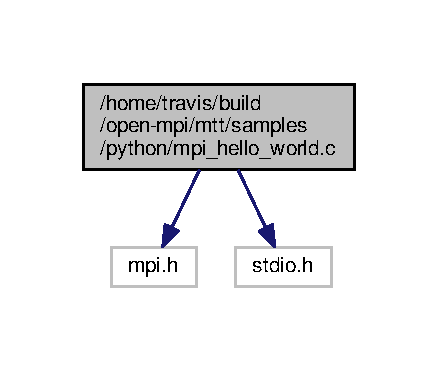
\includegraphics[width=210pt]{mpi__hello__world_8c__incl}
\end{center}
\end{figure}
\subsection*{Functions}
\begin{DoxyCompactItemize}
\item 
int \hyperlink{mpi__hello__world_8c_a3c04138a5bfe5d72780bb7e82a18e627}{main} (int argc, char $\ast$$\ast$argv)
\end{DoxyCompactItemize}


\subsection{Function Documentation}
\hypertarget{mpi__hello__world_8c_a3c04138a5bfe5d72780bb7e82a18e627}{\index{mpi\-\_\-hello\-\_\-world.\-c@{mpi\-\_\-hello\-\_\-world.\-c}!main@{main}}
\index{main@{main}!mpi_hello_world.c@{mpi\-\_\-hello\-\_\-world.\-c}}
\subsubsection[{main}]{\setlength{\rightskip}{0pt plus 5cm}int main (
\begin{DoxyParamCaption}
\item[{int}]{argc, }
\item[{char $\ast$$\ast$}]{argv}
\end{DoxyParamCaption}
)}}\label{mpi__hello__world_8c_a3c04138a5bfe5d72780bb7e82a18e627}


Definition at line 4 of file mpi\-\_\-hello\-\_\-world.\-c.


\hypertarget{mpitest_8ini}{\section{/home/travis/build/open-\/mpi/mtt/samples/python/mpitest.ini File Reference}
\label{mpitest_8ini}\index{/home/travis/build/open-\/mpi/mtt/samples/python/mpitest.\-ini@{/home/travis/build/open-\/mpi/mtt/samples/python/mpitest.\-ini}}
}
\subsection*{Namespaces}
\begin{DoxyCompactItemize}
\item 
\hyperlink{namespacempitest}{mpitest}
\end{DoxyCompactItemize}
\subsection*{Variables}
\begin{DoxyCompactItemize}
\item 
int \hyperlink{namespacempitest_aa0f43e6283b3889679e6631336f043d1}{mpitest.\-trial} = 0
\item 
int \hyperlink{namespacempitest_ac471d6a27e0973ff2ca6b08b1709963d}{mpitest.\-submit\-\_\-group\-\_\-results} = 1
\item 
\hyperlink{namespacempitest_ab3988561c8669a528d164bb087dfaba8}{mpitest.\-description} = Prototypetestconfigurationfile
\item 
\hyperlink{namespacempitest_aa707f637f52c6a7d6e9269de9fa926d3}{mpitest.\-platform} = bend-\/rsh
\item 
\hyperlink{namespacempitest_ad3586f81f11a42b438f3a012d4c2bf4e}{mpitest.\-plugin} = Git
\item 
\hyperlink{namespacempitest_aae573db72acd85d3ee46589c81be2d37}{mpitest.\-url} = https\-://github.\-com/open-\/mpi/ompi
\item 
\hyperlink{namespacempitest_a862f2676bbe33c7059e3a136b4b96ddc}{mpitest.\-username} = rhc54
\item 
\hyperlink{namespacempitest_a4d126335ef307f44645da8ff58e86927}{mpitest.\-pwfile} = rhcpasswd
\item 
\hyperlink{namespacempitest_afea79525dcdc90bf190e1fd794ba7377}{mpitest.\-parent} = Middleware\-Get\-:\-O\-M\-P\-I\-Master
\item 
\hyperlink{namespacempitest_a216b951ce28d23d25761486f09fdafa5}{mpitest.\-autogen\-\_\-cmd} = ./autogen.\-pl
\item 
\hyperlink{namespacempitest_ac530ff92b31cfd595a3fc3c3a82d7fc6}{mpitest.\-configure\-\_\-options} = -\/-\/enable-\/debug
\item 
int \hyperlink{namespacempitest_a59b1db518516dae2b5daace949760505}{mpitest.\-make\-\_\-options} = -\/j10
\item 
\hyperlink{namespacempitest_adb11b85868ea4bb66346873247ae5eee}{mpitest.\-subdir} = ibm
\item 
int \hyperlink{namespacempitest_a458e434e47470db96ce5fd267a120b69}{mpitest.\-merge\-\_\-stdout\-\_\-stderr} = 1
\item 
int \hyperlink{namespacempitest_a359e155a689c5604a331d2450976d0fa}{mpitest.\-stderr\-\_\-save\-\_\-lines} = 100
\item 
\hyperlink{namespacempitest_abda8feed4cda165ed145590c0c693826}{mpitest.\-middleware} = Middleware\-Build\-:\-O\-M\-P\-I\-Master
\item 
\hyperlink{namespacempitest_a47e2cc8f7e7a5ee1717d68777fd3c363}{mpitest.\-command} = mpirun-\/-\/oversubscribe
\item 
int \hyperlink{namespacempitest_ae35dc1081e40dfe24adccbc698417a69}{mpitest.\-np} = 16
\item 
list \hyperlink{namespacempitest_a91cdfabf3b22da570c284023ab54044f}{mpitest.\-options} = \mbox{[}\char`\"{}\char`\"{}, \char`\"{}-\/-\/novm\char`\"{}\mbox{]}
\item 
int \hyperlink{namespacempitest_a85870f11cfd9d17b34964ec12302c3bb}{mpitest.\-skipped} = 77
\item 
int \hyperlink{namespacempitest_a4a75d79ba591224da573cc9ab62552b6}{mpitest.\-stdout\-\_\-save\-\_\-lines} = 100
\item 
string \hyperlink{namespacempitest_afb14b0cb9c4139a5d3f2bf30599704ab}{mpitest.\-test\-\_\-dir} = \char`\"{}collective, communicator\char`\"{}
\item 
int \hyperlink{namespacempitest_aa789c1fae4dda8997bf0f7d9a794f877}{mpitest.\-max\-\_\-num\-\_\-tests} = 10
\item 
string \hyperlink{namespacempitest_a6fd83076e5878f8964800690579327d8}{mpitest.\-fail\-\_\-tests} = \char`\"{}environment/abort, environment/final\char`\"{}
\item 
\hyperlink{namespacempitest_a54920d94a964e18fe3ad81cbe8363c36}{mpitest.\-fail\-\_\-timeout} = max\-\_\-procs
\item 
string \hyperlink{namespacempitest_ac08f02520db8234e89010050fa3b76ea}{mpitest.\-skip\-\_\-tests} = \char`\"{}environment/init\-\_\-thread\-\_\-multiple,communicator/comm\-\_\-split\-\_\-f\char`\"{}
\item 
\hyperlink{namespacempitest_a7b80601152b8c206cc61614fcd09929a}{mpitest.\-filename} = mttresults.\-txt
\item 
\hyperlink{namespacempitest_a982b2dded1406d02564695cb5e756197}{mpitest.\-summary\-\_\-footer} =
\item 
\hyperlink{namespacempitest_a55ff433403a926c608140ebd229f138a}{mpitest.\-detail\-\_\-header} =
\item 
\hyperlink{namespacempitest_a3f742d28fd4486162a251a03685b28d0}{mpitest.\-detail\-\_\-footer} =
\item 
int \hyperlink{namespacempitest_a4ff3a6f6296976b6e0ed6249357c3542}{mpitest.\-textwrap} = 78
\end{DoxyCompactItemize}

\hypertarget{ompi__hello__world_8ini}{\section{/home/travis/build/open-\/mpi/mtt/samples/python/ompi\-\_\-hello\-\_\-world.ini File Reference}
\label{ompi__hello__world_8ini}\index{/home/travis/build/open-\/mpi/mtt/samples/python/ompi\-\_\-hello\-\_\-world.\-ini@{/home/travis/build/open-\/mpi/mtt/samples/python/ompi\-\_\-hello\-\_\-world.\-ini}}
}
\subsection*{Namespaces}
\begin{DoxyCompactItemize}
\item 
\hyperlink{namespaceompi__hello__world}{ompi\-\_\-hello\-\_\-world}
\end{DoxyCompactItemize}

\hypertarget{ompi__snapshot__seq_8ini}{\section{/home/travis/build/open-\/mpi/mtt/samples/python/ompi\-\_\-snapshot\-\_\-seq.ini File Reference}
\label{ompi__snapshot__seq_8ini}\index{/home/travis/build/open-\/mpi/mtt/samples/python/ompi\-\_\-snapshot\-\_\-seq.\-ini@{/home/travis/build/open-\/mpi/mtt/samples/python/ompi\-\_\-snapshot\-\_\-seq.\-ini}}
}
\subsection*{Namespaces}
\begin{DoxyCompactItemize}
\item 
\hyperlink{namespaceompi__snapshot__seq}{ompi\-\_\-snapshot\-\_\-seq}
\end{DoxyCompactItemize}
\subsection*{Variables}
\begin{DoxyCompactItemize}
\item 
\hyperlink{namespaceompi__snapshot__seq_a10070286ec527c9dfed8c210ca3917d7}{ompi\-\_\-snapshot\-\_\-seq.\-trial} = false
\item 
\hyperlink{namespaceompi__snapshot__seq_a8855b0a58b147479b623ede37dab8378}{ompi\-\_\-snapshot\-\_\-seq.\-scratch} = R\-E\-P\-L\-A\-C\-E\-\_\-\-M\-E\-\_\-\-P\-A\-T\-H\-\_\-\-T\-O\-\_\-\-S\-C\-R\-A\-T\-C\-H\-\_\-\-D\-I\-R
\item 
\hyperlink{namespaceompi__snapshot__seq_a918891e52aa1a572f039326981585a7a}{ompi\-\_\-snapshot\-\_\-seq.\-description} = Open\-M\-P\-Imaster
\item 
\hyperlink{namespaceompi__snapshot__seq_a300d0cc664225df572aad2518569d7bf}{ompi\-\_\-snapshot\-\_\-seq.\-platform} = R\-E\-P\-L\-A\-C\-E\-\_\-\-M\-E
\item 
\hyperlink{namespaceompi__snapshot__seq_a6293c71d0991763a4bad8b010e0e6ce2}{ompi\-\_\-snapshot\-\_\-seq.\-executor} = sequential
\item 
\hyperlink{namespaceompi__snapshot__seq_a4964274b9eb87e06a95ee1bef66604ef}{ompi\-\_\-snapshot\-\_\-seq.\-plugin} = O\-M\-P\-I\-\_\-\-Snapshot
\item 
\hyperlink{namespaceompi__snapshot__seq_a0af6b7793981b72fee25ffd1d077fd86}{ompi\-\_\-snapshot\-\_\-seq.\-url} = https\-://download.\-open-\/mpi.\-org/nightly/open-\/mpi/master
\item 
\hyperlink{namespaceompi__snapshot__seq_ab1bd70042bbcbfc640abba12010ed2b5}{ompi\-\_\-snapshot\-\_\-seq.\-version\-\_\-file} = R\-E\-P\-L\-A\-C\-E\-\_\-\-M\-E\-\_\-\-N\-A\-M\-E\-\_\-\-O\-F\-\_\-\-V\-E\-R\-S\-I\-O\-N\-\_\-\-F\-I\-L\-E
\item 
\hyperlink{namespaceompi__snapshot__seq_a464fbb2313394347fa064032378c5674}{ompi\-\_\-snapshot\-\_\-seq.\-mpi\-\_\-name} = ompi-\/nightly-\/master
\item 
\hyperlink{namespaceompi__snapshot__seq_a08a86b12770df9f65150ce521c8820b6}{ompi\-\_\-snapshot\-\_\-seq.\-parent} = Middleware\-Get\-:\-O\-M\-P\-I\-Master
\item 
\hyperlink{namespaceompi__snapshot__seq_affb396ef384900a98c5a943dd8817711}{ompi\-\_\-snapshot\-\_\-seq.\-configure\-\_\-options} = -\/-\/enable-\/debug
\item 
int \hyperlink{namespaceompi__snapshot__seq_a42ad6d7d01611e1404c4747596bad26f}{ompi\-\_\-snapshot\-\_\-seq.\-make\-\_\-options} = -\/j1
\item 
\hyperlink{namespaceompi__snapshot__seq_a9d517656629849b65e1dcefbcf9cfd73}{ompi\-\_\-snapshot\-\_\-seq.\-subdir} = ibm
\item 
int \hyperlink{namespaceompi__snapshot__seq_ad98d5c78e44526c2b86baccb081cd46e}{ompi\-\_\-snapshot\-\_\-seq.\-merge\-\_\-stdout\-\_\-stderr} = 1
\item 
int \hyperlink{namespaceompi__snapshot__seq_a4c1170c00e6cc51822262da67c07d721}{ompi\-\_\-snapshot\-\_\-seq.\-stderr\-\_\-save\-\_\-lines} = 100
\item 
\hyperlink{namespaceompi__snapshot__seq_a25acb4b0e7bb13ac146f46ae7f074689}{ompi\-\_\-snapshot\-\_\-seq.\-middleware} = Middleware\-Build\-:\-O\-M\-P\-I\-Master
\item 
\hyperlink{namespaceompi__snapshot__seq_a2e5939b3a3bd4bacecb7b4b33cad0313}{ompi\-\_\-snapshot\-\_\-seq.\-autogen\-\_\-cmd} = ./autogen.\-sh
\item 
\hyperlink{namespaceompi__snapshot__seq_a7ee776e6bd84fc7f42f758751ba25e1e}{ompi\-\_\-snapshot\-\_\-seq.\-command} = mpirun
\item 
int \hyperlink{namespaceompi__snapshot__seq_ac5c6ca602093f9742f1afbfc100f8cfd}{ompi\-\_\-snapshot\-\_\-seq.\-np} = 2
\item 
int \hyperlink{namespaceompi__snapshot__seq_a7261e8a10955a8c08df3d642714fb626}{ompi\-\_\-snapshot\-\_\-seq.\-skipped} = 77
\item 
int \hyperlink{namespaceompi__snapshot__seq_a0521277c015b3e1b74418fc58101d5d6}{ompi\-\_\-snapshot\-\_\-seq.\-stdout\-\_\-save\-\_\-lines} = 100
\item 
int \hyperlink{namespaceompi__snapshot__seq_a4a2554fd9d8c0df86eeaae67f5bc6867}{ompi\-\_\-snapshot\-\_\-seq.\-timeout} = 600
\item 
string \hyperlink{namespaceompi__snapshot__seq_ae15b0abc55bc72ce7a7a4ebe56fc2dfe}{ompi\-\_\-snapshot\-\_\-seq.\-test\-\_\-dir} = \char`\"{}collective, communicator, datatype, environment, group, info, io, onesided, pt2pt, random, topology\char`\"{}
\item 
int \hyperlink{namespaceompi__snapshot__seq_a8c173774cc05394e996dbb13e37d0322}{ompi\-\_\-snapshot\-\_\-seq.\-max\-\_\-num\-\_\-tests} = 10
\item 
string \hyperlink{namespaceompi__snapshot__seq_a1c6caf43d8724d112db736b1cc590bef}{ompi\-\_\-snapshot\-\_\-seq.\-fail\-\_\-tests} = \char`\"{}environment/abort, environment/final\char`\"{}
\item 
\hyperlink{namespaceompi__snapshot__seq_ac68ac424f71d3b098f0e5742e90083c1}{ompi\-\_\-snapshot\-\_\-seq.\-fail\-\_\-timeout} = max\-\_\-procs
\item 
string \hyperlink{namespaceompi__snapshot__seq_a0a1e6182d0b6b408fd0b3642c5b52556}{ompi\-\_\-snapshot\-\_\-seq.\-skip\-\_\-tests} = \char`\"{}environment/init\-\_\-thread\-\_\-multiple,communicator/comm\-\_\-split\-\_\-f\char`\"{}
\item 
\hyperlink{namespaceompi__snapshot__seq_ac375b04988441d39d7dbd8546bede172}{ompi\-\_\-snapshot\-\_\-seq.\-filename} = mttresults.\-txt
\item 
\hyperlink{namespaceompi__snapshot__seq_ae564d5d2ad344e6edd9fe25c04553c4f}{ompi\-\_\-snapshot\-\_\-seq.\-summary\-\_\-footer} =
\item 
\hyperlink{namespaceompi__snapshot__seq_aa8131df6b7e79ce54a5832a78a18226b}{ompi\-\_\-snapshot\-\_\-seq.\-detail\-\_\-header} =
\item 
\hyperlink{namespaceompi__snapshot__seq_a0238cbbb945d76de96b90e3cd058d356}{ompi\-\_\-snapshot\-\_\-seq.\-detail\-\_\-footer} =
\item 
int \hyperlink{namespaceompi__snapshot__seq_a81239e350a24a25aa3a329f330a267f4}{ompi\-\_\-snapshot\-\_\-seq.\-textwrap} = 78
\item 
\hyperlink{namespaceompi__snapshot__seq_aab43e86098df5461b6d69d6554bacf51}{ompi\-\_\-snapshot\-\_\-seq.\-realm} = O\-M\-P\-I
\item 
\hyperlink{namespaceompi__snapshot__seq_ad73553bb8a0851422895d9c7e8978b83}{ompi\-\_\-snapshot\-\_\-seq.\-username} = R\-E\-P\-L\-A\-C\-E\-\_\-\-M\-E
\item 
\hyperlink{namespaceompi__snapshot__seq_a6229810db63f8ab2e0598c9dc5da7a32}{ompi\-\_\-snapshot\-\_\-seq.\-password} = R\-E\-P\-L\-A\-C\-E\-\_\-\-M\-E
\end{DoxyCompactItemize}

\hypertarget{test_8ini}{\section{/home/travis/build/open-\/mpi/mtt/samples/python/test.ini File Reference}
\label{test_8ini}\index{/home/travis/build/open-\/mpi/mtt/samples/python/test.\-ini@{/home/travis/build/open-\/mpi/mtt/samples/python/test.\-ini}}
}
\subsection*{Namespaces}
\begin{DoxyCompactItemize}
\item 
\hyperlink{namespacetest}{test}
\end{DoxyCompactItemize}

%--- End generated contents ---

% Index
\newpage
\phantomsection
\addcontentsline{toc}{chapter}{Index}
\printindex

\end{document}
